% !Mode:: "TeX:UTF-8"
% !TEX encoding = UTF-8 Unicode

%----------------------------------------------------------------------------------------
% 机器翻译:基础与模型
% Machine Translation: Foundations and Models
%
% Copyright 2020
% 肖桐(xiaotong@mail.neu.edu.cn) 朱靖波 (zhujingbo@mail.neu.edu.cn)
%----------------------------------------------------------------------------------------

%----------------------------------------------------------------------------------------
%    CONFIGURATIONS
%----------------------------------------------------------------------------------------

\renewcommand\figurename{图}%将figure改为图
\renewcommand\tablename{表}%将figure改为图
\chapterimage{fig-NEU-6.jpg} % Chapter heading image

%----------------------------------------------------------------------------------------
%	CHAPTER 15
%----------------------------------------------------------------------------------------

\chapter{神经机器翻译结构优化}

\parinterval 模型结构的设计是机器翻译系统研发中最重要的工作之一。在神经机器翻译时代,虽然系统研发人员脱离了繁琐的特征工程,但是神经网络结构的设计仍然耗时耗力。无论是像循环神经网络、Transformer 这样的整体架构的设计,还是注意力机制等局部结构的设计,都对机器翻译性能有着很大的影响。

\parinterval 本章主要讨论神经机器翻译中结构优化的若干研究方向,包括:注意力机制的改进、网络连接优化及深层网络建模、基于树结构的模型、神经网络结构自动搜索等。这些内容可以指导神经机器翻译系统的深入优化,其中涉及的一些模型和方法也可以应用于其他自然语言处理任务。

%----------------------------------------------------------------------------------------
%    NEW SECTION
%----------------------------------------------------------------------------------------

\sectionnewpage
\section{注意力机制的改进}

\parinterval 注意力机制是神经机器翻译成功的关键。以Transformer模型为例,由于使用了自注意力机制,该模型展现出较高的训练并行性,同时在机器翻译、语言建模等任务上,该模型也取得了很好的表现。但是Transformer模型仍存在许多亟待解决的问题,例如,在处理长文本序列时(假设文本长度为$N$),自注意力机制的时间复杂度为$O(N^2)$,当$N$过大时翻译速度很低。此外,尽管Transformer模型的输入中包含了绝对位置编码表示,但是现有的自注意力机制仍然无法显性捕获局部窗口下不同位置之间的关系。而且注意力机制也需要更多样的手段进行特征提取,例如,采用多头或者多分支结构对不同空间特征进行提取。针对以上问题,本节将介绍注意力机制的优化策略,并重点讨论Transformer模型的若干改进方法。

%----------------------------------------------------------------------------------------
%    NEW SUB-SECTION
%----------------------------------------------------------------------------------------

\subsection{局部信息建模}\label{subsec-15.1.1}

\parinterval 使用循环神经网络进行序列建模时,每一个时刻的计算都依赖于上一时刻循环单元的状态。这种模式天然具有一定的时序性,同时具有{\small\bfnew{归纳偏置}}\index{归纳偏置}(Inductive Bias)\index{Inductive Bias}的特性\upcite{DBLP:journals/corr/abs-1806-01261},即每一时刻的状态仅仅基于当前时刻的输入和前一时刻的状态。这种归纳偏置的好处在于,模型并不需要对绝对位置进行建模,因此模型可以很容易处理任意长度的序列,即使测试样本显著长于训练样本。

\parinterval 但是,Transformer模型中的自注意力机制本身并不具有这种性质,而且它直接忽略了输入单元之间的位置关系。虽然,Transformer中引入了基于正余弦函数的绝对位置编码(见{\chaptertwelve}),但是该方法仍然无法显性区分局部依赖与长距离依赖\footnote[1]{局部依赖指当前位置与局部的相邻位置之间的联系。}。

\parinterval 针对上述问题,研究人员尝试引入“相对位置”信息,对原有的“绝对位置”信息进行补充,强化了局部依赖\upcite{Dai2019TransformerXLAL,Shaw2018SelfAttentionWR}。此外,由于模型中每一层均存在自注意力机制计算,因此模型捕获位置信息的能力也逐渐减弱,这种现象在深层模型中尤为明显。而利用相对位置编码能够把位置信息显性加入到每一层的注意力机制的计算中,进而强化深层模型的位置表示能力\upcite{li2020shallow}。图\ref{fig:15-1}对比了Transformer中绝对位置编码和相对位置编码方法。

%----------------------------------------------
\begin{figure}[htp]
\centering
\begin{tikzpicture}

\tikzstyle{Sanode} = [minimum height=1.1em,minimum width=7em,inner sep=3pt,rounded corners=1.5pt,draw,thick];
\tikzstyle{Resnode} = [minimum height=1.1em,minimum width=7em,inner sep=3pt,rounded corners=1.5pt,draw,thick];
\tikzstyle{ffnnode} = [minimum height=1.1em,minimum width=7em,inner sep=3pt,rounded corners=1.5pt,draw,thick];
\tikzstyle{outputnode} = [minimum height=1.4em,minimum width=7em,inner sep=3pt,rounded corners=1.5pt,draw,thick];
\tikzstyle{inputnode} = [minimum height=1.4em,minimum width=3.5em,inner sep=3pt,rounded corners=1.5pt,draw,fill=red!20,thick];
\tikzstyle{posnode} = [minimum height=1.4em,minimum width=3.5em,inner sep=3pt,rounded corners=1.5pt,draw,fill=black!10!white,thick];
\tikzstyle{standard} = [rounded corners=3pt];

\begin{scope}
\node [Sanode,anchor=west] (sa1) at (0,0) {\tiny{$\textbf{Self-Attention}$}};
\node [Resnode,anchor=south] (res1) at ([yshift=0.3em]sa1.north) {\tiny{$\textbf{Add \& LayerNorm}$}};
\node [ffnnode,anchor=south] (ffn1) at ([yshift=0.5em]res1.north) {\tiny{$\textbf{Feed Forward Network}$}};
\node [Resnode,anchor=south] (res2) at ([yshift=0.3em]ffn1.north) {\tiny{$\textbf{Add \& LayerNorm}$}};

\node [anchor=south,minimum height=1.4em,minimum width=7em] (dot1) at ([yshift=1.5em]res2.north) {\tiny{$\cdots$}};

\node [Sanode,anchor=south] (sa2) at ([yshift=1.5em]dot1.north) {\tiny{$\textbf{Self-Attention}$}};
\node [Resnode,anchor=south] (res3) at ([yshift=0.3em]sa2.north) {\tiny{$\textbf{Add \& LayerNorm}$}};
\node [ffnnode,anchor=south] (ffn2) at ([yshift=0.5em]res3.north) {\tiny{$\textbf{Feed Forward Network}$}};
\node [Resnode,anchor=south] (res4) at ([yshift=0.3em]ffn2.north) {\tiny{$\textbf{Add \& LayerNorm}$}};

\node [anchor=north west,font=\scriptsize,align=center,ublue] (l1) at ([xshift=0.1em]ffn1.north east) {第 \\ $1$ \\ 层};
\node [anchor=north west,font=\scriptsize,align=center,ublue] (l2) at ([xshift=0.1em]ffn2.north east) {第 \\ $n$ \\ 层};
\node [anchor=south east,font=\scriptsize] (l3) at ([yshift=3em]l1.north east) {};
\node [anchor=north east,font=\scriptsize,align=center,opacity=0.0] (l4) at ([xshift=0.1em]ffn1.north west) {第 \\ $1$ \\ 层};
\node [anchor=north east,font=\scriptsize,align=center,opacity=0.0] (l5) at ([xshift=0.1em]ffn2.north west) {第 \\ $n$ \\ 层};
\node [anchor=south west,font=\scriptsize] (l6) at ([yshift=3em]l4.north west) {};

\node [anchor=south west] (e1) at ([xshift=-1.4em,yshift=0.3em]res4.north west) {{编码器}};

\node [anchor=north,minimum height=0.1em,minimum width=0.1em] (set1) at ([xshift=0em,yshift=0.3em]sa1.south) {};
\node [anchor=north,minimum height=0.1em,minimum width=0.1em] (set2) at ([xshift=0em,yshift=0.3em]sa2.south) {};

\begin{pgfonlayer}{background}
	\node [rectangle,inner sep=0.6em,rounded corners=5pt,very thick,dotted,minimum height=1.4em,minimum width=3.5em,draw=red] [fit = (e1) (sa1) (l1) (l4) (set1)] (b4) {};
	\node [rectangle,inner sep=0.3em,rounded corners=5pt,very thick,dotted,draw=ublue,minimum height=1.4em,minimum width=7em] [fit = (l1) (sa1) (res2) (l4) (set1)] (b1) {};		
	\node [rectangle,inner sep=0.3em,rounded corners=5pt,very thick,dotted,draw=ublue,minimum height=1.4em,minimum width=7em] [fit = (dot1) (l3) (l6)] (b2) {};	
	\node [rectangle,inner sep=0.3em,rounded corners=5pt,very thick,dotted,draw=ublue,minimum height=1.4em,minimum width=7em] [fit = (l2) (sa2) (res4) (l5) (set2)] (b3) {};	
\end{pgfonlayer}

\node [inputnode,anchor=north west] (input1) at ([yshift=-1.6em,xshift=-0.5em]sa1.south west) {\tiny{$\textbf{Embedding}$}};
\node [] (add) at ([yshift=-2.2em,xshift=3.5em]sa1.south west) {$+$};
\node [posnode,anchor=north east] (pos1) at ([yshift=-1.6em,xshift=1.6em]sa1.south east) {\tiny{$\textbf{Absolute Position}$}};

\node [anchor=north] (wi) at ([yshift=-0.5em]pos1.south) {\scriptsize{词序信息}};

\draw [->] (wi.north) -- (pos1.south);
\draw [->] (add.north) -- (sa1.south);
\draw [->] (sa1.north) -- (res1.south);
\draw [->] (res1.north) -- (ffn1.south);
\draw [->] (ffn1.north) -- (res2.south);
\draw [->] (res2.north) -- ([yshift=-0.4em]dot1.south);
\draw [->] ([yshift=0.3em]dot1.north) -- (sa2.south);
\draw [->] (sa2.north) -- (res3.south);
\draw [->] (res3.north) -- (ffn2.south);
\draw [->] (ffn2.north) -- (res4.south);
\draw [->] (res4.north) -- ([yshift=1em]res4.north);

\draw[->,standard] ([yshift=-0.3em]sa1.south) -- ([xshift=-4em,yshift=-0.3em]sa1.south) -- ([xshift=-4em,yshift=2em]sa1.south) -- ([xshift=-3.5em,yshift=2em]sa1.south);
\draw[->,standard] ([yshift=0.2em]res1.north) -- ([xshift=-4em,yshift=0.2em]res1.north) -- ([xshift=-4em,yshift=2.5em]res1.north) -- ([xshift=-3.5em,yshift=2.5em]res1.north);

\draw[->,standard] ([yshift=-0.3em]sa2.south) -- ([xshift=-4em,yshift=-0.3em]sa2.south) -- ([xshift=-4em,yshift=2em]sa2.south) -- ([xshift=-3.5em,yshift=2em]sa2.south);
\draw[->,standard] ([yshift=0.2em]res3.north) -- ([xshift=-4em,yshift=0.2em]res3.north) -- ([xshift=-4em,yshift=2.5em]res3.north) -- ([xshift=-3.5em,yshift=2.5em]res3.north);

\begin{pgfonlayer}{background}
	\node [rectangle,inner sep=0.2em,rounded corners=1pt,very thick,dotted,fill=red!40] [fit = (input1) (pos1)] (box1) {};
\end{pgfonlayer}

\node [anchor=north,font=\small] (label) at ([yshift=-3em]add.south) {{(a)绝对位置编码}};

\end{scope}


\begin{scope}[xshift=2in]
\node [Sanode,anchor=west] (sa1) at (0,0) {\tiny{$\textbf{Self-Attention}$}};
\node [Resnode,anchor=south] (res1) at ([yshift=0.3em]sa1.north) {\tiny{$\textbf{Add \& LayerNorm}$}};
\node [ffnnode,anchor=south] (ffn1) at ([yshift=0.5em]res1.north) {\tiny{$\textbf{Feed Forward Network}$}};
\node [Resnode,anchor=south] (res2) at ([yshift=0.3em]ffn1.north) {\tiny{$\textbf{Add \& LayerNorm}$}};

\node [anchor=south,minimum height=1.4em,minimum width=7em] (dot1) at ([yshift=1.5em]res2.north) {\tiny{$\cdots$}};

\node [Sanode,anchor=south] (sa2) at ([yshift=1.5em]dot1.north) {\tiny{$\textbf{Self-Attention}$}};
\node [Resnode,anchor=south] (res3) at ([yshift=0.3em]sa2.north) {\tiny{$\textbf{Add \& LayerNorm}$}};
\node [ffnnode,anchor=south] (ffn2) at ([yshift=0.5em]res3.north) {\tiny{$\textbf{Feed Forward Network}$}};
\node [Resnode,anchor=south] (res4) at ([yshift=0.3em]ffn2.north) {\tiny{$\textbf{Add \& LayerNorm}$}};

\node [anchor=north west,font=\scriptsize,align=center,ublue] (l1) at ([xshift=0.1em]ffn1.north east) {第 \\ $1$ \\ 层};
\node [anchor=north west,font=\scriptsize,align=center,ublue] (l2) at ([xshift=0.1em]ffn2.north east) {第 \\ $n$ \\ 层};
\node [anchor=south east,font=\scriptsize] (l3) at ([yshift=3em]l1.north east) {};
\node [anchor=north east,font=\scriptsize,align=center,opacity=0.0] (l4) at ([xshift=0.1em]ffn1.north west) {第 \\ $1$ \\ 层};
\node [anchor=north east,font=\scriptsize,align=center,opacity=0.0] (l5) at ([xshift=0.1em]ffn2.north west) {第 \\ $n$ \\ 层};
\node [anchor=south west,font=\scriptsize] (l6) at ([yshift=3em]l4.north west) {};

\node [anchor=south west] (e1) at ([xshift=-1.4em,yshift=0.3em]res4.north west) {{编码器}};

\node [anchor=north,minimum height=0.1em,minimum width=0.1em] (set1) at ([xshift=0em,yshift=0.3em]sa1.south) {};
\node [anchor=north,minimum height=0.1em,minimum width=0.1em] (set2) at ([xshift=0em,yshift=0.3em]sa2.south) {};

\begin{pgfonlayer}{background}
	\node [rectangle,inner sep=0.6em,rounded corners=5pt,very thick,dotted,minimum height=1.4em,minimum width=3.5em,draw=red] [fit = (e1) (sa1) (l1) (l4) (set1)] (b4) {};
	\node [rectangle,inner sep=0.3em,rounded corners=5pt,very thick,dotted,draw=ublue,minimum height=1.4em,minimum width=7em] [fit = (l1) (sa1) (res2) (l4) (set1)] (b1) {};		
	\node [rectangle,inner sep=0.3em,rounded corners=5pt,very thick,dotted,draw=ublue,minimum height=1.4em,minimum width=7em] [fit = (dot1) (l3) (l6)] (b2) {};	
	\node [rectangle,inner sep=0.3em,rounded corners=5pt,very thick,dotted,draw=ublue,minimum height=1.4em,minimum width=7em] [fit = (l2) (sa2) (res4) (l5) (set2)] (b3) {};	
\end{pgfonlayer}

\node [inputnode,anchor=north west] (input1) at ([yshift=-1.6em,xshift=-0.5em]sa1.south west) {\tiny{Embedding}};
\node [] (add) at ([yshift=-2.2em,xshift=3.5em]sa1.south west) {$+$};
\node [posnode,anchor=north east] (pos1) at ([yshift=-1.6em,xshift=1.5em]sa1.south east) {\tiny{Absolute Position}};

\node [anchor=north] (wi) at ([yshift=-0.5em]pos1.south) {\scriptsize{词序信息}};

\node [posnode,anchor=west,font=\tiny,align=center] (pos2) at ([yshift=0em,xshift=1em]pos1.east) {Relative \\ Position 1};
\node [posnode,anchor=west,font=\tiny,align=center,minimum width=1em] (pos3) at ([yshift=0em,xshift=1em]pos2.east) {$\cdots$};
\node [posnode,anchor=west,font=\tiny,align=center] (pos4) at ([yshift=0em,xshift=1em]pos3.east) {Relative \\ Position $n$};

\draw [->] (wi.north) -- (pos1.south);
\draw [->] (add.north) -- (sa1.south);
\draw [->] (sa1.north) -- (res1.south);
\draw [->] (res1.north) -- (ffn1.south);
\draw [->] (ffn1.north) -- (res2.south);
\draw [->] (res2.north) -- ([yshift=-0.4em]dot1.south);
\draw [->] ([yshift=0.3em]dot1.north) -- (sa2.south);
\draw [->] (sa2.north) -- (res3.south);
\draw [->] (res3.north) -- (ffn2.south);
\draw [->] (ffn2.north) -- (res4.south);
\draw [->] (res4.north) -- ([yshift=1em]res4.north);

\draw[->,standard] ([yshift=-0.3em]sa1.south) -- ([xshift=-4em,yshift=-0.3em]sa1.south) -- ([xshift=-4em,yshift=2em]sa1.south) -- ([xshift=-3.5em,yshift=2em]sa1.south);
\draw[->,standard] ([yshift=0.2em]res1.north) -- ([xshift=-4em,yshift=0.2em]res1.north) -- ([xshift=-4em,yshift=2.5em]res1.north) -- ([xshift=-3.5em,yshift=2.5em]res1.north);

\draw[->,standard] ([yshift=-0.3em]sa2.south) -- ([xshift=-4em,yshift=-0.3em]sa2.south) -- ([xshift=-4em,yshift=2em]sa2.south) -- ([xshift=-3.5em,yshift=2em]sa2.south);
\draw[->,standard] ([yshift=0.2em]res3.north) -- ([xshift=-4em,yshift=0.2em]res3.north) -- ([xshift=-4em,yshift=2.5em]res3.north) -- ([xshift=-3.5em,yshift=2.5em]res3.north);

\draw[->,standard] ([xshift=0em]wi.east) -- ([xshift=3.25em,yshift=0em]wi.east) -- ([xshift=-0em,yshift=0em]pos2.south);
\draw[->,standard] ([xshift=0em]wi.east) -- ([xshift=6.78em,yshift=0em]wi.east) -- ([xshift=-0em,yshift=0em]pos3.south);
\draw[->,standard] ([xshift=0em]wi.east) -- ([xshift=10.3em,yshift=0em]wi.east) -- ([xshift=-0em,yshift=0em]pos4.south);
\draw[->,standard] ([xshift=0em]pos2.north) -- ([xshift=0em,yshift=2.1em]pos2.north) -- ([xshift=-0em,yshift=0em]sa1.east);
\draw[->,standard] ([xshift=0em]pos3.north) -- ([xshift=0em,yshift=9.6em]pos3.north) -- ([xshift=-0em,yshift=0em]dot1.east);
\draw[->,standard] ([xshift=0em]pos4.north) -- ([xshift=0em,yshift=12.3em]pos4.north) -- ([xshift=-0em,yshift=0em]sa2.east);


\begin{pgfonlayer}{background}
	\node [rectangle,inner sep=0.2em,rounded corners=1pt,very thick,dotted,fill=red!40] [fit = (pos2) (pos3) (pos4)] (box1) {};
\end{pgfonlayer}

\node [anchor=north,font=\small] (label) at ([xshift=4em,yshift=-3em]add.south) {{(b)相对位置编码}};

\end{scope}


\end{tikzpicture}
\caption{绝对位置编码和相对位置编码}
\label{fig:15-1}
\end{figure}
%-------------------------------------------

%----------------------------------------------------------------------------------------
%    NEW SUBSUB-SECTION
%----------------------------------------------------------------------------------------

\subsubsection{1. 位置编码}\label{subsubsec-15.1.1}

\parinterval 在介绍相对位置编码之前,首先简要回顾一下自注意力机制的计算流程(见{\chaptertwelve})。对于Transformer模型中的某一层神经网络,可以定义:
\begin{eqnarray}
\mathbi{Q} & = & \mathbi{x} \mathbi{W}_Q \\
\mathbi{K} & = & \mathbi{x} \mathbi{W}_K \\
\mathbi{V} & = & \mathbi{x} \mathbi{W}_V
\label{eq:15-3}
\end{eqnarray}

\noindent 其中,$\mathbi{x}$为上一层的输出\footnote[2]{这里,$\mathbi{K}$、$\mathbi{Q}$、$\mathbi{V}$的定义与{\chaptertwelve}略有不同,因为在这里的$\mathbi{K}$、$\mathbi{Q}$、$\mathbi{V}$ 是指对注意力模型输入进行线性变换后的结果,而{\chaptertwelve}中$\mathbi{K}$、$\mathbi{Q}$、$\mathbi{V}$直接表示输入。但是,这两种描述方式本质上是一样的,区别仅仅在于对输入的线性变化是放在输入自身中描述,还是作为输入之后的一个额外操作。},$\mathbi{W}_Q$、$\mathbi{W}_K$、$\mathbi{W}_V$为模型参数,它们可以通过自动学习得到。此时,对于整个模型输入的向量序列$\mathbi{x}=\{\mathbi{x}_1,\ldots,\mathbi{x}_m\}$,通过点乘计算,可以得到当前位置$i$和序列中所有位置间的关系,记为$\mathbi{z}_{i} $,计算公式如下:
\begin{eqnarray}
\mathbi{z}_{i} &=& \sum_{j=1}^m \alpha_{ij}(\mathbi{x}_j \mathbi{W}_V)
\label{eq:15-4}
\end{eqnarray}

\noindent 这里,$\mathbi{z}_{i}$可以被看做是输入序列的线性加权表示结果。权重$\alpha_{ij}$通过Softmax函数得到:
\begin{eqnarray}
\alpha_{ij} &=& \frac{\exp (\mathbi{e}_{ij})}{\sum_{k=1}^{m}\exp (\mathbi{e}_{ik})}
\label{eq:15-5}
\end{eqnarray}

\noindent 进一步,$\mathbi{e}_{ij}$被定义为:
\begin{eqnarray}
\mathbi{e}_{ij} &=& \frac{(\mathbi{x}_i \mathbi{W}_Q){(\mathbi{x}_j \mathbi{W}_K)}^{T}}{\sqrt{d_k}}
\label{eq:15-6}
\end{eqnarray}

\noindent 其中,$d_k$为模型中隐层的维度\footnote[3]{在多头注意力中,$d_k$为经过多头分割后每个头的维度。}。$\mathbi{e}_{ij}$实际上就是$\mathbi{Q}$和$\mathbi{K}$的向量积缩放后的一个结果。

\parinterval 基于上述描述,相对位置模型可以按如下方式实现:

\begin{itemize}
\vspace{0.5em}
\item {\small\bfnew{相对位置编码}}\index{相对位置编码}(Relative Positional Representation)\index{Relative Positional Representation}\upcite{Shaw2018SelfAttentionWR}。核心思想是在能够捕获全局依赖的自注意力机制中引入相对位置信息。该方法可以有效补充绝对位置编码的不足,甚至完全取代绝对位置编码。对于Transformer模型中的任意一层,假设$\mathbi{x}_i$和$\mathbi{x}_j$是位置$i$和$j$的输入向量(也就是来自上一层位置$i$和$j$的输出向量),二者的位置关系可以通过向量$\mathbi{a}_{ij}^V$ 和$\mathbi{a}_{ij}^K$来表示,定义如下:
\begin{eqnarray}
\mathbi{a}_{ij}^K &=& \mathbi{w}^K_{\textrm{clip}(j-i,k)} \label{eq:15-7} \\
\mathbi{a}_{ij}^V &=& \mathbi{w}^V_{\textrm{clip}(j-i,k)} \label{eq:15-8} \\
\textrm{clip}(x,k) &=& \max(-k,\min(k,x)) 
\label{eq:15-9}
\end{eqnarray}

\noindent 其中,$\mathbi{w}^K \in \mathbb{R}^{d_k}$和$\mathbi{w}^V \in \mathbb{R}^{d_k}$是模型中可学习的参数矩阵;$\textrm{clip}(\cdot,\cdot)$表示截断操作,由公式\eqref{eq:15-9}定义。可以看出,$\mathbi{a}^K$ 与$\mathbi{a}^V$ 是根据输入的相对位置信息(由$\textrm{clip}(j-i,k)$确定)对$\mathbi{w}^K$和$\mathbi{w}^V$进行查表得到的向量,即相对位置表示,如图\ref{fig:15-2}所示。这里通过预先设定的最大相对位置$k$,强化模型对以当前词为中心的左右各$k$ 个词的注意力计算。因此,最终的窗口大小为$2k + 1$。 对于边缘位置窗口大小不足$2k$的单词,采用了裁剪的机制,即只对有效的临近词进行建模。此时,注意力模型的计算可以调整为:
\begin{eqnarray}
\mathbi{z}_{i} &=& \sum_{j=1}^m \alpha_{ij}(\mathbi{x}_j \mathbi{W}_V + \mathbi{a}_{ij}^V)
\label{eq:15-10}
\end{eqnarray}

%----------------------------------------------
\begin{figure}[htp]
\centering
\vspace{-1em}
\begin{tikzpicture}

\tikzstyle{node1} = [anchor=center,draw,minimum height=2em,minimum width=2em,inner sep=0pt,fill=ugreen!80]
\tikzstyle{node2} = [anchor=center,draw,minimum height=2em,minimum width=2em,inner sep=0pt,fill=ugreen!50]
\tikzstyle{node3} = [anchor=center,draw,minimum height=2em,minimum width=2em,inner sep=0pt,fill=ugreen!20]
\tikzstyle{node4} = [anchor=center,draw,minimum height=2em,minimum width=2em,inner sep=0pt]
\tikzstyle{node5} = [anchor=center,draw,minimum height=2em,minimum width=2em,inner sep=0pt,fill=teal!20]
\tikzstyle{node6} = [anchor=center,draw,minimum height=2em,minimum width=2em,inner sep=0pt,fill=teal!50]
\tikzstyle{node7} = [anchor=center,draw,minimum height=2em,minimum width=2em,inner sep=0pt,fill=teal!80]

\begin{scope}[scale=1.0]
\foreach \i / \j / \k / \z in
    {0/6/1/-3, 1/6/1/-3, 2/6/1/-3, 3/6/1/-3, 4/6/2/-2, 5/6/3/-1, 6/6/4/0,
    0/5/1/-3, 1/5/1/-3, 2/5/1/-3, 3/5/2/-2, 4/5/3/-1, 5/5/4/0, 6/5/5/1,
    0/4/1/-3, 1/4/1/-3, 2/4/2/-2, 3/4/3/-1, 4/4/4/0, 5/4/5/1, 6/4/6/2,
    0/3/1/-3, 1/3/2/-2, 2/3/3/-1, 3/3/4/0, 4/3/5/1, 5/3/6/2, 6/3/7/3,
    0/2/2/-2, 1/2/3/-1, 2/2/4/0, 3/2/5/1, 4/2/6/2, 5/2/7/3, 6/2/7/3,
    0/1/3/-1, 1/1/4/0, 2/1/5/1, 3/1/6/2, 4/1/7/3, 5/1/7/3, 6/1/7/3,
    0/0/4/0, 1/0/5/1, 2/0/6/2, 3/0/7/3, 4/0/7/3, 5/0/7/3, 6/0/7/3}
    \node[node\k] (a\i\j) at (2*1em*\i + 0*0em,2*1em*\j + 0*0em) {$\mathbi{w}_{\z}$};

\foreach \i / \j / \k in
    {0/6/1, 0/5/2, 0/4/3, 0/3/4, 0/2/5, 0/1/6, 0/0/7}
    \node[anchor=east] (n\k) at ([xshift=-0.5em,yshift=0em]a\i\j.west) {\j};

\foreach \i / \j / \k in
    {0/0/8, 1/0/9, 2/0/10, 3/0/11, 4/0/12, 5/0/13, 6/0/14}
    \node[anchor=north] (n\k) at ([xshift=-0em,yshift=-0.5em]a\i\j.south) {\i};

\node [anchor=east] (l1) at ([xshift=-0.3em,yshift=0em]n8.west) {$j$};
\node [anchor=north] (l2) at ([xshift=0em,yshift=-0em]n7.south) {$i$};

%\node [anchor=north] (n1) at ([xshift=0em,yshift=0em]a00.south west) {};

\end{scope}
\end{tikzpicture}
\caption{相对位置权重$\mathbi{a}_{ij}$\upcite{DBLP:conf/emnlp/HuangLXX20}}
\setlength{\belowcaptionskip}{-2em}
\label{fig:15-2}
\end{figure}
%-------------------------------------------

\noindent 相比于公式\eqref{eq:15-4},公式\eqref{eq:15-10}在计算$\mathbi{z}_i$时引入了额外的向量$\mathbi{a}_{ij}^V$,用它来表示位置$i$与位置$j$之间的相对位置信息。同时在计算注意力权重时对$\mathbi{K}$进行修改,同样引入了$\mathbi{a}_{ij}^K$向量表示位置$i$与位置$j$之间的相对位置。在公式\eqref{eq:15-6}的基础上,注意力权重的计算方式调整为:
\begin{eqnarray}
\mathbi{e}_{ij} &=& \frac{\mathbi{x}_i \mathbi{W}_Q{(\mathbi{x}_j \mathbi{W}_K + \mathbi{a}_{ij}^K )}^{T}}{\sqrt{d_k}} \nonumber \\
&=& \frac{\mathbi{x}_i \mathbi{W}_Q{(\mathbi{x}_j \mathbi{W}_K)}^{T} + \mathbi{x}_i \mathbi{W}_Q{(\mathbi{a}_{ij}^K )}^{T}}{\sqrt{d_k}}
\label{eq:15-11}
\end{eqnarray}

\noindent 可以注意到,公式\eqref{eq:15-10}和公式\eqref{eq:15-11}将位置编码信息直接暴露给每一层注意力机制的计算,而不是像标准Transformer中只将其作为整个模型的输入。

\vspace{0.5em}
\item {\small\bfnew{Transformer-XL}}\upcite{Dai2019TransformerXLAL}。在Transformer中,模型的输入由词嵌入表示与绝对位置编码组成,例如,对于输入层有,$\mathbi{x}_i = \mathbi{E}_{x_i} + \mathbi{U}_i$,$\mathbi{x}_j=\mathbi{E}_{x_j} + \mathbi{U}_j$,其中$\mathbi{E}_{x_i} $和$\mathbi{E}_{x_j} $表示词嵌入,$\mathbi{U}_i$和$\mathbi{U}_j$表示绝对位置编码(正余弦函数)。将$\mathbi{x}_i$与$\mathbi{x}_j$代入公式\eqref{eq:15-6}中可以得到:
\begin{eqnarray}
\mathbi{e}_{ij} &=& \frac{(\mathbi{E}_{x_i} + \mathbi{U}_i)\mathbi{W}_Q{((\mathbi{E}_{x_j} + \mathbi{U}_j)\mathbi{W}_K)}^{T}}{\sqrt{d_k}}
\label{eq:15-12}
\end{eqnarray}

\noindent 这里使用$A_{ij}^{\rm abs}$表示公式\eqref{eq:15-12}中等式右侧的分子部分,并对其进行展开:
\begin{eqnarray}
A_{ij}^{\rm abs} &=& \underbrace{\mathbi{E}_{x_i}\mathbi{W}_Q\mathbi{W}_{K}^{T}\mathbi{E}_{x_j}^{T}}_{\textrm{(a)}} + \underbrace{\mathbi{E}_{x_i}\mathbi{W}_Q\mathbi{W}_{K}^{T}\mathbi{U}_{j}^{T}}_{\textrm{(b)}} + \nonumber \\
& & \underbrace{\mathbi{U}_i\mathbi{W}_Q\mathbi{W}_{K}^{T}\mathbi{E}_{x_j}^{T}}_{\textrm{(c)}} + \underbrace{\mathbi{U}_i\mathbi{W}_Q\mathbi{W}_{K}^{T}\mathbi{U}_{j}^{T}}_{\textrm{(d)}}
\label{eq:15-13}
\end{eqnarray}

\noindent 其中,${\rm abs}$代表使用绝对位置编码计算得到的$A_{ij}$,$\mathbi{W}_Q$与$\mathbi{W}_K$表示线性变换矩阵。为了引入相对位置信息,可以将公式\eqref{eq:15-13}修改为如下形式:
\begin{eqnarray}
A_{ij}^{\rm rel} &=& \underbrace{\mathbi{E}_{x_i}\mathbi{W}_Q\mathbi{W}_{K}^{T}\mathbi{E}_{x_j}^{T}}_{\textrm{(a)}} + \underbrace{\mathbi{E}_{x_i}\mathbi{W}_Q\mathbi{W}_{K}^{T}\mathbi{R}_{i-j}^{T}}_{\textrm{(b)}} + \nonumber \\
& & \underbrace{\mathbi{u}\mathbi{W}_{K,E}^{T}\mathbi{E}_{x_j}^{T}}_{\textrm{(c)}} + \underbrace{\mathbi{v}\mathbi{W}_{K,R}^{T}\mathbi{R}_{i-j}^{T}}_{\textrm{(d)}}
\label{eq:15-14}
\end{eqnarray}

\noindent 其中,$A_{ij}^{\rm rel}$为使用相对位置编码后位置$i$与$j$关系的表示结果,$\mathbi{R}$是一个固定的正弦矩阵。不同于公式\eqref{eq:15-13},公式\eqref{eq:15-14}对(c)中的$\mathbi{E}_{x_j}^{T}$与(d)中的$\mathbi{R}_{i-j}^{T}$采用了不同的映射矩阵,分别为$\mathbi{W}_{K,E}^{T}$和$\mathbi{W}_{K,R}^{T}$,这两项分别代表了键$\mathbi{K}$中的词嵌入表示和相对位置编码表示,并且由于此时只采用了相对位置编码,因此公式\eqref{eq:15-14}在(c)与(d)部分使用了$\mathbi{u}$和$\mathbi{v}$两个可学习的矩阵代替$\mathbi{U}_i\mathbi{W}_Q$与$\mathbi{U}_i\mathbi{W}_Q$,即查询$\mathbi{Q}$中的绝对位置编码部分。此时公式中各项的含义为:(a)表示位置$i$与位置$j$之间词嵌入的相关性,可以看作是基于内容的表示,(b)表示基于内容的位置偏置,(c)表示全局内容的偏置,(d)表示全局位置的偏置。公式\eqref{eq:15-13}中的(a)、(b)两项与前面介绍的绝对位置编码一致\upcite{Shaw2018SelfAttentionWR},并针对相对位置编码引入了额外的线性变换矩阵。同时,这种方法兼顾了全局内容偏置和全局位置偏置,可以更好地利用正余弦函数的归纳偏置特性。

\vspace{0.5em}
\item {\small\bfnew{结构化位置编码}}\index{基于结构化位置编码}(Structural Position Representations)\index{Structural Position Representations}\upcite{DBLP:conf/emnlp/WangTWS19a}。 例如,可以通过对输入句子进行依存句法分析得到句法树,根据叶子结点在句法树中的深度来表示其绝对位置,并在此基础上利用相对位置编码的思想计算节点之间的相对位置信息。

\vspace{0.5em}
\item {\small\bfnew{基于连续动态系统}}\index{基于连续动态系统}(Continuous Dynamic Model)\index{Continuous Dynamic Model}{\small\bfnew{的位置编码}}\upcite{Liu2020LearningTE}。使用神经常微分方程{\small\bfnew{求解器}}\index{求解器}(Solver)\index{Solver}来建模位置信息\upcite{DBLP:conf/nips/ChenRBD18},模型具有更好的归纳偏置能力,可以处理变长的输入序列,同时能够从不同的数据中进行自适应学习。
\vspace{0.5em}
\end{itemize}

%----------------------------------------------------------------------------------------
%    NEW SUBSUB-SECTION
%----------------------------------------------------------------------------------------

\subsubsection{2. 注意力分布约束}

\parinterval 局部注意力机制一直是机器翻译中受关注的研究方向\upcite{DBLP:journals/corr/LuongPM15}。通过对注意力权重的可视化,可以观测到不同位置的词受关注的程度相对平滑。这样的建模方式利于全局建模,但一定程度上分散了注意力,导致模型忽略了邻近单词之间的关系。为了提高模型对局部信息的感知,有以下几种方法:

\begin{itemize}
\vspace{0.5em}
\item {\small\bfnew{引入高斯约束}}\upcite{Yang2018ModelingLF}。如图\ref{fig:15-3}所示,这类方法的核心思想是引入可学习的高斯分布$\mathbi{G}$作为局部约束,与注意力权重进行融合。

%----------------------------------------------
\begin{figure}[htp]
\centering
%%%------------------------------------------------------------------------------------------------------------

\begin{center}
\begin{tikzpicture}

\tikzstyle{cirnode}=[circle,inner sep=4pt,draw]
\tikzstyle{colnode}=[fill=ugreen!30,inner sep=0.1pt]

\tikzstyle{show}=[fill=red,circle,inner sep=0.5pt]

\begin{scope}

\node [anchor=north west,circle,inner sep=4pt] (c1) at (0, 0) {};

\draw[-,dotted] ([xshift=-1em,yshift=-0.5em]c1.south)--([xshift=9.3em,yshift=-0.5em]c1.south);
\draw[-,dotted] ([xshift=-1em,yshift=-2em]c1.south)--([xshift=9.3em,yshift=-2em]c1.south);
\draw[-,dotted] ([xshift=-1em,yshift=-3.5em]c1.south)--([xshift=9.3em,yshift=-3.5em]c1.south);
\draw[-,dotted] ([xshift=-1em,yshift=-5em]c1.south)--([xshift=9.3em,yshift=-5em]c1.south);

\node [anchor=south,colnode,minimum height=1.6em,minimum width=1em] (b1) at ([xshift=0em,yshift=-5em]c1.south) {};
\node [anchor=south,colnode,minimum height=4.1em,minimum width=1em] (b2) at ([xshift=1.67em,yshift=0em]b1.south) {};
\node [anchor=south,colnode,minimum height=0.8em,minimum width=1em] (b3) at ([xshift=1.67em,yshift=0em]b2.south) {};
\node [anchor=south,colnode,minimum height=0.4em,minimum width=1em] (b4) at ([xshift=1.67em,yshift=0em]b3.south) {};
\node [anchor=south,colnode,minimum height=0.15em,minimum width=1em] (b5) at ([xshift=1.67em,yshift=0em]b4.south) {};
\node [anchor=south,colnode,minimum height=0.15em,minimum width=1em] (b6) at ([xshift=1.67em,yshift=0em]b5.south) {};

{\scriptsize
\node [anchor=center] (n1) at ([xshift=0em,yshift=-1em]b1.south){\color{orange}It};
\node [anchor=west] (n2) at ([xshift=1em,yshift=0em]n1.east){\color{ugreen}is};
\node [anchor=west] (n3) at ([xshift=1em,yshift=-0.1em]n2.east){a};
\node [anchor=west] (n4) at ([xshift=0.5em,yshift=0.1em]n3.east){nice};
\node [anchor=west] (n5) at ([xshift=0em,yshift=-0.1em]n4.east){day};
\node [anchor=west] (n6) at ([xshift=-0.1em,yshift=0em]n5.east){today};
}

\node [anchor=north] (l1) at ([xshift=1em,yshift=-1em]n3.south){\small {(a)原始分布}};

\draw[-,very thick] ([xshift=1.2em,yshift=2.4em]b6.north)--([xshift=1.7em,yshift=1.9em]b6.north);
\draw[-,very thick] ([xshift=1.2em,yshift=1.9em]b6.north)--([xshift=1.7em,yshift=2.4em]b6.north);

\end{scope}

\begin{scope}[xshift=4.4cm,yshift=0em]

\node [anchor=north west,circle,inner sep=4pt] (c1) at (0, 0) {};

\draw[-,dotted] ([xshift=-1em,yshift=-0.5em]c1.south)--([xshift=9.3em,yshift=-0.5em]c1.south);
\draw[-,dotted] ([xshift=-1em,yshift=-2em]c1.south)--([xshift=9.3em,yshift=-2em]c1.south);
\draw[-,dotted] ([xshift=-1em,yshift=-3.5em]c1.south)--([xshift=9.3em,yshift=-3.5em]c1.south);
\draw[-,dotted] ([xshift=-1em,yshift=-5em]c1.south)--([xshift=9.3em,yshift=-5em]c1.south);

\node [anchor=south,inner sep=0.1pt,minimum height=1.6em,minimum width=1em] (b1) at ([xshift=0em,yshift=-5em]c1.south) {};
\node [anchor=south,inner sep=0.1pt,minimum height=4.1em,minimum width=1em] (b2) at ([xshift=1.67em,yshift=0em]b1.south) {};
\node [anchor=south,inner sep=0.1pt,minimum height=0.8em,minimum width=1em] (b3) at ([xshift=1.67em,yshift=0em]b2.south) {};
\node [anchor=south,inner sep=0.1pt,minimum height=0.4em,minimum width=1em] (b4) at ([xshift=1.67em,yshift=0em]b3.south) {};
\node [anchor=south,inner sep=0.1pt,minimum height=0.15em,minimum width=1em] (b5) at ([xshift=1.67em,yshift=0em]b4.south) {};
\node [anchor=south,inner sep=0.1pt,minimum height=0.15em,minimum width=1em] (b6) at ([xshift=1.67em,yshift=0em]b5.south) {};

{\scriptsize
\node [anchor=center] (n1) at ([xshift=0em,yshift=-1em]b1.south){\color{orange}It};
\node [anchor=west] (n2) at ([xshift=0.5em,yshift=0em]n1.east){is};
\node [anchor=west] (n3) at ([xshift=0.5em,yshift=-0.1em]n2.east){a};
\node [anchor=west] (n4) at ([xshift=0.5em,yshift=0.1em]n3.east){\color{blue}nice};
\node [anchor=west] (n5) at ([xshift=0em,yshift=-0.1em]n4.east){day};
\node [anchor=west] (n6) at ([xshift=0em,yshift=0em]n5.east){today};
}

\draw [-,blue!60,thick] ([xshift=-1em,yshift=-4.7em]c1.south) cos(2em,-4em) sin (4.4em,-1.7em) cos(7.3em,-4em) sin([xshift=9.3em,yshift=-4.7em]c1.south);
%\draw[-,blue!60,thick] ([xshift=-1em,yshift=-4.7em]c1.south)..controls (3.8em,-6em) and (3.9em,3.6em)..([xshift=9.3em,yshift=-4.3em]c1.south);

\node [anchor=north] (l1) at ([xshift=1em,yshift=-1em]n3.south){\small {(b)高斯分布}};

\draw[-,very thick] ([xshift=1.2em,yshift=2.2em]b6.north)--([xshift=1.7em,yshift=2.2em]b6.north);
\draw[-,very thick] ([xshift=1.2em,yshift=1.9em]b6.north)--([xshift=1.7em,yshift=1.9em]b6.north);

\node [anchor=south] (t1) at ([xshift=0em,yshift=5.7em]n4.north){$D_i$};
\draw[->] ([xshift=0em,yshift=0em]t1.west)--([xshift=-1em,yshift=0em]t1.west);
\draw[->] ([xshift=0em,yshift=0em]t1.east)--([xshift=1em,yshift=0em]t1.east);
\draw[-] ([xshift=1em,yshift=-0.5em]t1.east)--([xshift=1em,yshift=0.5em]t1.east);
\draw[-] ([xshift=-1em,yshift=-0.5em]t1.west)--([xshift=-1em,yshift=0.5em]t1.west);

\end{scope}

\begin{scope}[xshift=8.8cm,yshift=0em]

\node [anchor=north west,circle,inner sep=4pt] (c1) at (0, 0) {};

\draw[-,dotted] ([xshift=-1em,yshift=-0.5em]c1.south)--([xshift=9.3em,yshift=-0.5em]c1.south);
\draw[-,dotted] ([xshift=-1em,yshift=-2em]c1.south)--([xshift=9.3em,yshift=-2em]c1.south);
\draw[-,dotted] ([xshift=-1em,yshift=-3.5em]c1.south)--([xshift=9.3em,yshift=-3.5em]c1.south);
\draw[-,dotted] ([xshift=-1em,yshift=-5em]c1.south)--([xshift=9.3em,yshift=-5em]c1.south);

\node [anchor=south,colnode,minimum height=0.85em,minimum width=1em] (b1) at ([xshift=0em,yshift=-5em]c1.south) {};
\node [anchor=south,colnode,minimum height=4.2em,minimum width=1em] (b2) at ([xshift=1.67em,yshift=0em]b1.south) {};
\node [anchor=south,colnode,minimum height=3.2em,minimum width=1em] (b3) at ([xshift=1.67em,yshift=0em]b2.south) {};
\node [anchor=south,colnode,minimum height=4.2em,minimum width=1em] (b4) at ([xshift=1.67em,yshift=0em]b3.south) {};
\node [anchor=south,colnode,minimum height=1.4em,minimum width=1em] (b5) at ([xshift=1.67em,yshift=0em]b4.south) {};
\node [anchor=south,colnode,minimum height=0.35em,minimum width=1em] (b6) at ([xshift=1.67em,yshift=0em]b5.south) {};

{\scriptsize
\node [anchor=center] (n1) at ([xshift=0em,yshift=-1em]b1.south){\color{orange}It};
\node [anchor=west] (n2) at ([xshift=1em,yshift=0em]n1.east){\color{ugreen}is};
\node [anchor=west] (n3) at ([xshift=1em,yshift=-0.1em]n2.east){\color{ugreen}a};
\node [anchor=west] (n4) at ([xshift=0.5em,yshift=0.1em]n3.east){\color{ugreen}nice};
\node [anchor=west] (n5) at ([xshift=0em,yshift=-0.1em]n4.east){day};
\node [anchor=west] (n6) at ([xshift=-0.1em,yshift=0em]n5.east){today};
}

\node [anchor=north] (l1) at ([xshift=1em,yshift=-1em]n3.south){\small {(c)修改后的分布}};

\end{scope}


\end{tikzpicture}
\end{center}
\caption{融合高斯分布的注意力分布}
\label{fig:15-3}
\end{figure}
%-------------------------------------------

\noindent 具体的形式如下:
\begin{eqnarray}
\mathbi{e}_{ij} &=& \frac{(\mathbi{x}_i \mathbi{W}_Q){(\mathbi{x}_j \mathbi{W}_K)}^{T}}{\sqrt{d_k}} + G_{ij}
\label{eq:15-15}
\end{eqnarray}

\noindent 其中,$G_{ij}$表示位置$j$和预测的中心位置$P_i$之间的关联程度,$G_{ij}$是$\mathbi{G}$中的一个元素,$\mathbi{G} \in \mathbb{R}^{m\times m}$。计算公式如下:
\begin{eqnarray}
G_{ij} &=& - \frac{{(j - P_i)}^2}{2\sigma_i^2}
\label{eq:15-16}
\end{eqnarray}

\noindent 其中,$\sigma_i$表示偏差,被定义为第$i$个词的局部建模窗口大小$D_i$的一半,即$\sigma_i = \frac{D_i}{2}$。中心位置$P_i$和局部建模窗口$D_i$的计算方式如下:
\begin{eqnarray}
\begin{pmatrix} P_i \\ D_i \end{pmatrix} &=& m \cdot \textrm{Sigmoid}(\begin{pmatrix} p_i \\ v_i \end{pmatrix})
\label{eq:15-17}
\end{eqnarray}

\noindent 其中,$m$表示序列长度,$p_i$和$v_i$为计算的中间结果,被定义为:
\begin{eqnarray}
p_i &=& \mathbi{I}_p^T\textrm{Tanh}(\mathbi{W}_p\mathbi{Q}_i) \\
v_i &=& \mathbi{I}_d^T\textrm{Tanh}(\mathbi{W}_d\mathbi{Q}_i)
\label{eq:15-19}
\end{eqnarray}

\noindent 其中,$\mathbi{W}_p$、$\mathbi{W}_d$、$\mathbi{I}_p$、$\mathbi{I}_d$均为模型中可学习的参数矩阵。

\vspace{0.5em}
\item {\small\bfnew{多尺度局部建模}}\upcite{DBLP:conf/aaai/GuoQLXZ20}。不同于上述方法直接作用于注意力权重,多尺度局部建模通过赋予多头不一样的局部感受野,间接地引入局部约束(图\ref{fig:15-4})。

%----------------------------------------------
\begin{figure}[htp]
\centering
\begin{tikzpicture}
\begin{scope}

\tikzstyle{cirnode}=[rectangle,rounded corners=2pt,minimum height=2em,minimum width=3em,font=\footnotesize,draw,fill=blue!20,thick]
\tikzstyle{recnode}=[rectangle,rounded corners=2pt,inner sep=0mm,minimum height=1.8em,minimum width=6em]

\node [anchor=west,cirnode] (n1) at (0, 0) {$\mathbi{h}_{i-2}^l$};
\node [anchor=west,cirnode] (n2) at ([xshift=1.2em,yshift=0em]n1.east) {$\mathbi{h}_{i-1}^l$};
\node [anchor=west,cirnode] (n3) at ([xshift=1.2em,yshift=0em]n2.east) {$\mathbi{h}_{i}^l$};
\node [anchor=west,cirnode] (n4) at ([xshift=1.2em,yshift=0em]n3.east) {$\mathbi{h}_{i+1}^l$};
\node [anchor=west,cirnode] (n5) at ([xshift=1.2em,yshift=0em]n4.east) {$\mathbi{h}_{i+2}^l$};

\begin{pgfonlayer}{background}
\node [anchor=center,red!30,minimum height=3.5em,minimum width=21em,very thick,draw] (c3) at ([xshift=0em,yshift=0em]n3.center) {};
\node [anchor=center,ugreen!30,minimum height=3em,minimum width=13em,very thick,draw] (c2) at ([xshift=0em,yshift=0em]n3.center) {};
\node [anchor=center,orange!30,minimum height=2.5em,minimum width=4em,very thick,draw] (c1) at ([xshift=0em,yshift=0em]n3.center) {};
\end{pgfonlayer}

\node [anchor=south,recnode,fill=red!30] (r1) at ([xshift=-3.5em,yshift=2.5em]n2.north) {$\textrm{head}_1$};
\node [anchor=south,recnode,fill=orange!30] (r2) at ([xshift=0em,yshift=2.5em]n3.north) {$\textrm{head}_2$};
\node [anchor=south,recnode,fill=ugreen!30] (r3) at ([xshift=3.5em,yshift=2.5em]n4.north) {$\textrm{head}_3$};

\node [anchor=south,cirnode] (n6) at ([xshift=0em,yshift=1.5em]r2.north) {$\mathbi{h}_{i}^{l+1}$};

\draw [->,very thick,orange!30] ([xshift=0em,yshift=0em]c1.north) -- ([xshift=0em,yshift=0em]r2.south);
\draw [->,very thick,ugreen!30] ([xshift=3em,yshift=0em]c2.north)..controls +(north:1.5em) and +(south:1.5em)..([xshift=0em,yshift=0em]r3.south);
\draw [->,very thick,red!30] ([xshift=-3em,yshift=0em]c3.north)..controls +(north:1.5em) and +(south:1.5em)..([xshift=0em,yshift=0em]r1.south);

\draw [->,red!30,very thick] ([xshift=0em,yshift=0em]r1.north) -- ([xshift=-0.1em,yshift=-0.05em]n6.south);
\draw [->,orange!30,very thick] ([xshift=0em,yshift=0em]r2.north) -- ([xshift=0em,yshift=0em]n6.south);
\draw [->,ugreen!30,very thick] ([xshift=0em,yshift=0em]r3.north) -- ([xshift=0.1em,yshift=-0.05em]n6.south);

\end{scope}
\end{tikzpicture}
\caption{多尺度局部建模\upcite{DBLP:conf/aaai/GuoQLXZ20}}
\label{fig:15-4}
\end{figure}
%-------------------------------------------

\noindent 于是,在计算第$i$个词对第$j$个词的相关系数时,通过超参数$\omega$控制实际的感受野为$j-\omega,\ldots,j+\omega$,注意力计算中$\mathbi{e}_{ij}$的计算方式与公式\eqref{eq:15-6}相同,权重$\alpha_{ij}$的具体计算公式为:
\begin{eqnarray}
\alpha_{ij} &=& \frac{\exp (\mathbi{e}_{ij})}{\sum_{k=j-\omega}^{j+\omega}\exp (\mathbi{e}_{ik})}
\label{eq:15-20}
\end{eqnarray}

\noindent 之后在计算注意力输出时同样利用上述思想进行局部约束:
\begin{eqnarray}
\mathbi{z}_{i} &=& \sum_{j=j-\omega}^{j+\omega} \alpha_{ij}(\mathbi{x}_j \mathbi{W}_V)
\label{eq:15-22}
\end{eqnarray}

\noindent 其中,约束的具体作用范围会根据实际句长进行一定的裁剪,通过对不同的头设置不同的超参数来控制感受野的大小,最终实现多尺度局部建模。

\vspace{0.5em}
\end{itemize}

\parinterval 值得注意的是上述两种添加局部约束的方法都更适用于Transformer模型的底层网络。这是由于模型离输入更近的层更倾向于捕获局部信息\upcite{Jawahar2019WhatDB,Yang2018ModelingLF},伴随着神经网络的加深,模型更倾向于逐渐加强全局建模的能力。类似的结论在针对BERT模型的解释性研究工作中也有论述\upcite{Jawahar2019WhatDB,DBLP:conf/emnlp/Ethayarajh19}。

%----------------------------------------------------------------------------------------
%    NEW SUBSUB-SECTION
%----------------------------------------------------------------------------------------

\subsubsection{3. 卷积 vs 注意力}

\parinterval 第十一章已经提到,卷积神经网络能够很好地捕捉序列中的局部信息。因此,充分地利用卷积神经网络的特性,也是一种进一步优化注意力模型的思路。常见的做法是在注意力模型中引入卷积操作,甚至用卷积操作替换注意力模型,如:

\begin{itemize}
\vspace{0.5em}
\item {\small\bfnew{使用轻量卷积和动态卷积神经网络}}\upcite{Wu2019PayLA,DBLP:conf/interspeech/GulatiQCPZYHWZW20}。比如,分别在编码器和解码器利用轻量卷积或动态卷积神经网络(见{\chapternine})替换Transformer的自注意力机制,同时保留解码器的编码-解码注意力机制,一定程度上加强了模型对局部信息的建模能力,同时提高了计算效率。
\vspace{0.5em}
\item {\small\bfnew{使用1维卷积注意力网络}}\upcite{DBLP:journals/corr/abs-1904-03107}(图\ref{fig:15-5}(b))。可以使用一维的卷积自注意力网络(1D-CSAN)将关注的范围限制在相近的元素窗口中。其形式上十分简单,只需预先设定好局部建模的窗口大小$D$,并在进行注意力权重计算和对Value值进行加权求和时,将其限制在设定好的窗口范围内。
\vspace{0.5em}
\item {\small\bfnew{使用2维卷积注意力网络}}(图\ref{fig:15-5}(c))。在一维卷积注意力网络的基础上,对多个注意力头之间的信息进行交互建模,打破了注意力头之间的界限。1D-CSAN的关注区域为$1\times D$,当将其扩展为二维矩形$D \times N$,长和宽分别为局部窗口的大小和参与建模的自注意力头的个数。这样,模型可以计算某个头中的第$i$个元素和另一个头中的第$j$个元素之间的相关性系数,实现了对不同子空间之间关系的建模,所得到的注意力分布表示了头之间的依赖关系。

%----------------------------------------------
\begin{figure}[htp]
\centering
\begin{tikzpicture}

\tikzstyle{elementnode} = [anchor=center,draw=gray,minimum size=0.6em,inner sep=0.1pt]

\begin{scope}[scale=1.0]
\foreach \i / \j in
    {0/4, 1/4, 2/4, 3/4, 4/4, 5/4, 6/4, 7/4,
    0/3, 1/3, 2/3, 3/3, 4/3, 5/3, 6/3, 7/3,
    0/2, 1/2, 2/2, 3/2, 4/2, 5/2, 6/2, 7/2,
    0/1, 1/1, 2/1, 3/1, 4/1, 5/1, 6/1, 7/1,
    0/0, 1/0, 2/0, 3/0, 4/0, 5/0, 6/0, 7/0}
    \node[elementnode] (a\i\j) at (0.6em*\i,0.6em*\j) {};

\foreach \i / \j in
    {0/4, 1/4, 2/4, 3/4, 4/4, 5/4, 6/4, 7/4,
    0/3, 1/3, 2/3, 3/3, 4/3, 5/3, 6/3, 7/3,
    0/2, 1/2, 2/2, 3/2, 4/2, 5/2, 6/2, 7/2,
    0/1, 1/1, 2/1, 3/1, 4/1, 5/1, 6/1, 7/1,
    0/0, 1/0, 2/0, 3/0, 4/0, 5/0, 6/0, 7/0}
    \node[elementnode,fill=orange!15] (b\i\j) at (0.6em*\i+5.5em,0.6em*\j) {};


\node [anchor=south west,minimum height=0.5em,minimum width=4.8em,inner sep=0.1pt,very thick,blue!60,draw] (n1) at ([xshift=0em,yshift=0em]a01.south west) {};
\node [anchor=north west,minimum height=0.5em,minimum width=4.8em,inner sep=0.1pt,very thick,red!60,draw] (n2) at ([xshift=0em,yshift=0em]a02.north west) {};
\node [anchor=west,minimum height=0.6em,minimum width=0.6em,inner sep=0.1pt,very thick,blue!60,draw] (n3) at ([xshift=0em,yshift=0em]b21.west) {};
\node [anchor=west,minimum height=0.6em,minimum width=0.6em,inner sep=0.1pt,very thick,red!60,draw] (n4) at ([xshift=0em,yshift=0em]b42.west) {};

\draw [-,very thick,dotted,blue!60] ([xshift=0em,yshift=0em]n1.south east) -- ([xshift=0em,yshift=0em]n3.south west);
\draw [-,very thick,dotted,blue!60] ([xshift=0em,yshift=0em]n1.north east) -- ([xshift=0em,yshift=0em]n3.north west);
\draw [-,very thick,dotted,red!60] ([xshift=0em,yshift=0em]n2.south east) -- ([xshift=0em,yshift=0em]n4.south west);
\draw [-,very thick,dotted,red!60] ([xshift=0em,yshift=0em]n2.north east) -- ([xshift=0em,yshift=0em]n4.north west);

\node [anchor=north] (l1) at ([xshift=0.5em,yshift=-1em]a70.south){\footnotesize {(a)标准自注意力模型}};
\node [anchor=south,rotate=90] (l2) at ([xshift=0em,yshift=0em]a02.west){\scriptsize {注意力头}};
\node [anchor=south] (l2) at ([xshift=0em,yshift=0em]a44.north){\scriptsize {句子长度}};

\end{scope}

\begin{scope}[scale=1.0,xshift=4.6cm]
\foreach \i / \j in
    {0/4, 1/4, 2/4, 3/4, 4/4, 5/4, 6/4, 7/4,
    0/3, 1/3, 2/3, 3/3, 4/3, 5/3, 6/3, 7/3,
    0/2, 1/2, 2/2, 3/2, 4/2, 5/2, 6/2, 7/2,
    0/1, 1/1, 2/1, 3/1, 4/1, 5/1, 6/1, 7/1,
    0/0, 1/0, 2/0, 3/0, 4/0, 5/0, 6/0, 7/0}
    \node[elementnode] (a\i\j) at (0.6em*\i,0.6em*\j) {};

\foreach \i / \j in
    {0/4, 1/4, 2/4, 3/4, 4/4, 5/4, 6/4, 7/4,
    0/3, 1/3, 2/3, 3/3, 4/3, 5/3, 6/3, 7/3,
    0/2, 1/2, 2/2, 3/2, 4/2, 5/2, 6/2, 7/2,
    0/1, 1/1, 2/1, 3/1, 4/1, 5/1, 6/1, 7/1,
    0/0, 1/0, 2/0, 3/0, 4/0, 5/0, 6/0, 7/0}
    \node[elementnode,fill=orange!15] (b\i\j) at (0.6em*\i+5.5em,0.6em*\j) {};


\node [anchor=south west,minimum height=0.5em,minimum width=3em,inner sep=0.1pt,very thick,blue!60,draw] (n1) at ([xshift=0em,yshift=0em]a01.south west) {};
\node [anchor=north west,minimum height=0.5em,minimum width=3em,inner sep=0.1pt,very thick,red!60,draw] (n2) at ([xshift=0em,yshift=0em]a22.north west) {};
\node [anchor=west,minimum height=0.6em,minimum width=0.6em,inner sep=0.1pt,very thick,blue!60,draw] (n3) at ([xshift=0em,yshift=0em]b21.west) {};
\node [anchor=west,minimum height=0.6em,minimum width=0.6em,inner sep=0.1pt,very thick,red!60,draw] (n4) at ([xshift=0em,yshift=0em]b42.west) {};

\draw [-,very thick,dotted,blue!60] ([xshift=0em,yshift=0em]n1.south east) -- ([xshift=0em,yshift=0em]n3.south west);
\draw [-,very thick,dotted,blue!60] ([xshift=0em,yshift=0em]n1.north east) -- ([xshift=0em,yshift=0em]n3.north west);
\draw [-,very thick,dotted,red!60] ([xshift=0em,yshift=0em]n2.south east) -- ([xshift=0em,yshift=0em]n4.south west);
\draw [-,very thick,dotted,red!60] ([xshift=0em,yshift=0em]n2.north east) -- ([xshift=0em,yshift=0em]n4.north west);

\node [anchor=north] (l1) at ([xshift=0.5em,yshift=-1em]a70.south){\footnotesize {(b)一维卷积注意力模型}};
\node [anchor=south,rotate=90] (l2) at ([xshift=0em,yshift=0em]a02.west){\scriptsize {注意力头}};
\node [anchor=south] (l2) at ([xshift=0em,yshift=0em]a44.north){\scriptsize {句子长度}};

\end{scope}

\begin{scope}[scale=1.0,xshift=9.2cm]
\foreach \i / \j in
    {0/4, 1/4, 2/4, 3/4, 4/4, 5/4, 6/4, 7/4,
    0/3, 1/3, 2/3, 3/3, 4/3, 5/3, 6/3, 7/3,
    0/2, 1/2, 2/2, 3/2, 4/2, 5/2, 6/2, 7/2,
    0/1, 1/1, 2/1, 3/1, 4/1, 5/1, 6/1, 7/1,
    0/0, 1/0, 2/0, 3/0, 4/0, 5/0, 6/0, 7/0}
    \node[elementnode] (a\i\j) at (0.6em*\i,0.6em*\j) {};

\foreach \i / \j in
    {0/4, 1/4, 2/4, 3/4, 4/4, 5/4, 6/4, 7/4,
    0/3, 1/3, 2/3, 3/3, 4/3, 5/3, 6/3, 7/3,
    0/2, 1/2, 2/2, 3/2, 4/2, 5/2, 6/2, 7/2,
    0/1, 1/1, 2/1, 3/1, 4/1, 5/1, 6/1, 7/1,
    0/0, 1/0, 2/0, 3/0, 4/0, 5/0, 6/0, 7/0}
    \node[elementnode,fill=orange!15] (b\i\j) at (0.6em*\i+5.5em,0.6em*\j) {};


\node [anchor=south west,minimum height=1.8em,minimum width=3em,inner sep=0.1pt,very thick,blue!60,draw] (n1) at ([xshift=0em,yshift=0em]a00.south west) {};
\node [anchor=north west,minimum height=1.8em,minimum width=3em,inner sep=0.1pt,very thick,red!60,draw] (n2) at ([xshift=0em,yshift=0em]a23.north west) {};
\node [anchor=west,minimum height=0.6em,minimum width=0.6em,inner sep=0.1pt,very thick,blue!60,draw] (n3) at ([xshift=0em,yshift=0em]b21.west) {};
\node [anchor=west,minimum height=0.6em,minimum width=0.6em,inner sep=0.1pt,very thick,red!60,draw] (n4) at ([xshift=0em,yshift=0em]b42.west) {};

\draw [-,very thick,dotted,blue!60] ([xshift=0em,yshift=0em]n1.south east) -- ([xshift=0em,yshift=0em]n3.south west);
\draw [-,very thick,dotted,blue!60] ([xshift=0em,yshift=0em]n1.north east) -- ([xshift=0em,yshift=0em]n3.north west);
\draw [-,very thick,dotted,red!60] ([xshift=0em,yshift=0em]n2.south east) -- ([xshift=0em,yshift=0em]n4.south west);
\draw [-,very thick,dotted,red!60] ([xshift=0em,yshift=0em]n2.north east) -- ([xshift=0em,yshift=0em]n4.north west);

\node [anchor=north] (l1) at ([xshift=0.5em,yshift=-1em]a70.south){\footnotesize {(c)二维卷积注意力模型}};
\node [anchor=south,rotate=90] (l2) at ([xshift=0em,yshift=0em]a02.west){\scriptsize {注意力头}};
\node [anchor=south] (l2) at ([xshift=0em,yshift=0em]a44.north){\scriptsize {句子长度}};

\end{scope}
\end{tikzpicture}
\caption{卷积注意力模型示意图\upcite{DBLP:journals/corr/abs-1904-03107}}
\label{fig:15-5}
\end{figure}
%-------------------------------------------
\end{itemize}

%----------------------------------------------------------------------------------------
%    NEW SUB-SECTION
%----------------------------------------------------------------------------------------

\subsection{多分支结构}

\parinterval 在神经网络模型中,可以使用多个平行的组件从不同角度捕捉输入的特征,这种结构被称为{\small\bfnew{多分支}}\index{多分支}(Multi-branch)\index{Multi-branch}结构。多分支结构在图像处理领域被广泛应用\upcite{DBLP:conf/cvpr/XieGDTH17},在许多人工设计或者自动搜索获得的神经网络结构中也有它的身影\upcite{DBLP:conf/icml/SoLL19,DBLP:conf/emnlp/YanMZ20,DBLP:journals/corr/abs-2006-10270}。

\parinterval 在自然语言处理领域,多分支结构同样也有很多应用。比如,{\chapterten}介绍过,为了更好地对源语言进行表示,编码器可以采用双向循环神经网络。这种模型就可以被看作一个两分支的结构,分别用来建模正向序列和反向序列的表示,之后将这两种表示进行拼接得到更丰富的序列表示结果。另一个典型的例子是{\chaptertwelve}介绍的多头注意力机制。在Transformer 模型中,多头注意力将输入向量分割成多个子向量,然后分别进行点乘注意力的计算,最后再将多个输出的子向量拼接后通过线性变换进行不同子空间信息的融合。在这个过程中,多个不同的头对应着不同的特征空间,可以捕捉到不同的特征信息。

\parinterval 近几年,在Transformer的结构基础上,研究人员探索了更为丰富的多分支结构。下面介绍几种在Transformer模型中引入多分支结构的方法:

\begin{itemize}
\vspace{0.5em}
\item {\small\bfnew{基于权重的方法}}\upcite{DBLP:journals/corr/abs-1711-02132}。其主要思想是在多头自注意力机制的基础上保留不同表示空间的特征。传统方法使用级联操作并通过线性映射矩阵来融合不同头之间的信息,而基于权重的Transformer直接利用线性映射将维度为$d_k$ 的向量表示映射到$d_{\rm model}$维的向量。之后,将这个$d_{\rm model}$维向量分别送入每个分支中的前馈神经网络,最后对不同分支的输出进行线性加权。但是,这种模型的计算复杂度要大于标准的Transformer模型。
\vspace{0.5em}
\item {\small\bfnew{基于多分支注意力的方法}}\upcite{DBLP:journals/corr/abs-2006-10270}。不同于基于权重的Transformer模型,多分支注意力模型直接利用每个分支独立地进行自注意力模型的计算(图\ref{fig:15-6})。同时为了避免结构相同的多个多头注意力机制之间的协同适应,这种模型使用Dropout方法在训练过程中以一定的概率随机地丢弃一些分支。

%----------------------------------------------
\begin{figure}[htp]
\centering
%%%------------------------------------------------------------------------------------------------------------
%%% 调序模型1:基于距离的调序
\begin{center}
\begin{tikzpicture}

\tikzstyle{manode}=[rectangle,inner sep=0mm,minimum height=1.8em,minimum width=10em,rounded corners=5pt,thick,draw,fill=teal!30]
\tikzstyle{ffnnode}=[rectangle,inner sep=0mm,minimum height=1.8em,minimum width=3em,rounded corners=5pt,thick,fill=red!30,draw]
\tikzstyle{lnnode}=[rectangle,inner sep=0mm,minimum height=2em,minimum width=2.5em,rounded corners=5pt,thick,fill=green!30,draw]

\begin{scope}[]

\node [anchor=east,circle,fill=black,inner sep = 2pt] (n1) at (-0, 0) {};
\node [anchor=west,draw,circle,inner sep=5pt,thick] (n2) at ([xshift=13em,yshift=0em]n1.east){};
\node [anchor=west,lnnode] (n3) at ([xshift=1.5em,yshift=0em]n2.east){LN};
\node [anchor=west,circle,fill=black,inner sep=2pt] (n4) at ([xshift=1.5em,yshift=0em]n3.east){};
\node [anchor=west,draw,circle,inner sep=5pt,thick] (n5) at ([xshift=5em,yshift=0em]n4.east){};
\node [anchor=west,lnnode] (n6) at ([xshift=1.5em,yshift=0em]n5.east){LN};

\node [anchor=west,manode] (a1) at ([xshift=1.5em,yshift=2em]n1.east){Multi-Head Attention};
\node [anchor=south] (a2) at ([xshift=0em,yshift=0.2em]a1.north){$\cdots$};
\node [anchor=south,manode] (a3) at ([xshift=0em,yshift=0.2em]a2.north){Multi-Head Attention};

\node [anchor=west,ffnnode] (f1) at ([xshift=1em,yshift=2em]n4.east){FFN};


\draw[->,thick] ([xshift=-1em,yshift=0em]n1.west)--([xshift=0em,yshift=0em]n1.west);
\draw[->,thick] ([xshift=0em,yshift=0em]n1.east)--([xshift=0em,yshift=0em]n2.west);
\draw[->,thick] ([xshift=0em,yshift=0em]n2.east)--([xshift=0em,yshift=0em]n3.west);
\draw[->,thick] ([xshift=0em,yshift=0em]n3.east)--([xshift=0em,yshift=0em]n4.west);
\draw[->,thick] ([xshift=0em,yshift=0em]n4.east)--([xshift=0em,yshift=0em]n5.west);
\draw[->,thick] ([xshift=0em,yshift=0em]n5.east)--([xshift=0em,yshift=0em]n6.west);
\draw[->,thick] ([xshift=0em,yshift=0em]n6.east)--([xshift=1em,yshift=0em]n6.east);

\draw[->,thick] ([xshift=0em,yshift=0em]n1.east)--([xshift=0em,yshift=0em]a1.west);
\draw[->,thick] ([xshift=0em,yshift=0em]n1.east)--([xshift=0em,yshift=0em]a3.west);
\draw[->,thick] ([xshift=0em,yshift=0em]n4.east)--([xshift=0em,yshift=0em]f1.west);

\draw[->,thick,ublue,dashed] ([xshift=0em,yshift=0em]a1.east)--([xshift=0em,yshift=0em]n2.west);
\draw[->,thick,ublue,dashed] ([xshift=0em,yshift=0em]a3.east)--([xshift=0em,yshift=0em]n2.west);
\draw[->,thick,ublue,dashed] ([xshift=0em,yshift=0em]f1.east)--([xshift=0em,yshift=0em]n5.west);

\node [anchor=west,ublue,font=\footnotesize,align=left] (w1) at ([xshift=5em,yshift=-0.5em]a2.east){以概率\\$p$丢弃};
\node [anchor=west,ublue,font=\footnotesize,align=left] (w2) at ([xshift=0.5em,yshift=0em]f1.east){以概率\\$p$丢弃};

\draw[-,thick] ([xshift=0em,yshift=0em]n2.west)--([xshift=-0em,yshift=0em]n2.east);
\draw[-,thick] ([xshift=0em,yshift=0em]n2.south)--([xshift=-0em,yshift=-0em]n2.north);

\draw[-,thick] ([xshift=0em,yshift=0em]n5.west)--([xshift=-0em,yshift=0em]n5.east);
\draw[-,thick] ([xshift=0em,yshift=0em]n5.south)--([xshift=-0em,yshift=-0em]n5.north);

\end{scope}
\end{tikzpicture}
\end{center}
\caption{多分支注意力模型}
\label{fig:15-6}
\end{figure}
%-------------------------------------------

\vspace{0.5em}
\item {\small\bfnew{基于多单元的方法}}。例如,为了进一步加强不同分支的作用,基于多单元的Transformer模型进行了序列不同位置表示结果的交换,或使用不同的掩码策略对不同分支的输入进行扰动,保证分支间的多样性与互补性\upcite{DBLP:conf/emnlp/YanMZ20}。本质上,所谓的多单元思想与集成学习十分相似,类似于在训练过程中同时训练多个编码器。此外,通过增大子单元之间的结构差异性也能够进一步增大分支之间的多样性\upcite{李北2019面向神经机器翻译的集成学习方法分析}。
\vspace{0.5em}
\end{itemize}

\parinterval 此外,在\ref{subsec-15.1.1}节中曾提到过,利用卷积神经网络可以与自注意力机制形成互补。类似的想法在多分支结构中也有体现。如图\ref{fig:15-7}所示,可以使用自注意力机制和卷积神经网络分别提取全局和局部两种依赖关系\upcite{DBLP:conf/iclr/WuLLLH20}。具体的做法是将输入的特征向量切分成等同维度的两部分,之后分别送入两个分支进行计算。其中,全局信息使用自注意力机制进行提取,局部信息使用轻量卷积网络进行提取\upcite{Wu2019PayLA}。此外,由于每个分支的维度只有原始的一半,采用并行计算方式可以显著提升系统的运行速度。

%----------------------------------------------
\begin{figure}[htp]
\centering
%%%------------------------------------------------------------------------------------------------------------
%%% 调序模型1:基于距离的调序
\begin{center}
\begin{tikzpicture}

\tikzstyle{manode}=[rectangle,inner sep=0mm,minimum height=4em,minimum width=4em,rounded corners=5pt,thick,draw,fill=blue!30]
\tikzstyle{ffnnode}=[rectangle,inner sep=0mm,minimum height=1.8em,minimum width=6em,rounded corners=5pt,thick,fill=red!30,draw]
\tikzstyle{ebnode}=[rectangle,inner sep=0mm,minimum height=1.8em,minimum width=10em,rounded corners=5pt,thick,fill=green!30,draw]

\begin{scope}[]

\node [anchor=west,inner sep=0mm,minimum height=1.8em] (f1) at (0, 0){input};
\node [anchor=south,ebnode] (e1) at ([xshift=0em,yshift=1em]f1.north){Embedding};
\node [anchor=south west,manode] (a1) at ([xshift=0em,yshift=1em]e1.north west){Attention};
\node [anchor=south east,manode] (c1) at ([xshift=0em,yshift=1em]e1.north east){Conv};
\node [anchor=south west,ebnode] (e2) at ([xshift=0em,yshift=1em]a1.north west){Embedding};
\node [anchor=south,draw,circle,inner sep=4pt] (add1) at ([xshift=0em,yshift=0.5em]e2.north){};
\node [anchor=south,ffnnode] (f2) at ([xshift=0em,yshift=0.5em]add1.north){FFN};
\node [anchor=south,inner sep=0mm,minimum height=1.8em] (op) at ([xshift=0em,yshift=0.5em]f2.north){output};


\draw[->,thick] ([xshift=0em,yshift=-0.3em]f1.north)--([xshift=0em,yshift=0em]e1.south);
\draw[->,thick] ([xshift=0em,yshift=-1em]a1.south)--([xshift=0em,yshift=0em]a1.south);
\draw[->,thick] ([xshift=0em,yshift=-1em]c1.south)--([xshift=0em,yshift=0em]c1.south);
\draw[->,thick] ([xshift=0em,yshift=0em]a1.north)--([xshift=0em,yshift=1em]a1.north);
\draw[->,thick] ([xshift=0em,yshift=0em]c1.north)--([xshift=0em,yshift=1em]c1.north);
\draw[-,thick] ([xshift=0em,yshift=0em]e2.north)--([xshift=0em,yshift=0em]add1.south);
\draw[->,thick] ([xshift=0em,yshift=0em]add1.north)--([xshift=0em,yshift=0em]f2.south);
\draw[->,thick] ([xshift=0em,yshift=0em]f2.north)--([xshift=0em,yshift=0.3em]op.south);


\draw[-] ([xshift=0em,yshift=0em]add1.west)--([xshift=-0em,yshift=0em]add1.east);
\draw[-] ([xshift=0em,yshift=0em]add1.south)--([xshift=-0em,yshift=-0em]add1.north);


\draw[->,thick,rectangle,rounded corners=5pt] ([xshift=0em,yshift=0.5em]f1.north)--([xshift=-6em,yshift=0.5em]f1.north)--([xshift=-5.45em,yshift=0em]add1.west)--([xshift=0em,yshift=0em]add1.west);


\end{scope}
\end{tikzpicture}
\end{center}
\caption{基于自注意力和卷积神经网络的2分支结构}
\label{fig:15-7}
\end{figure}
%-------------------------------------------

%----------------------------------------------------------------------------------------
%    NEW SUB-SECTION
%----------------------------------------------------------------------------------------

\subsection{引入循环机制}

\parinterval 虽然Transformer模型完全摒弃了循环单元与卷积单元,仅通过位置编码来区分序列中的不同位置。但是,循环神经网络也非常适用于处理序列结构,且其结构成熟、易于优化。因此,有研究人员尝试将其与Transformer模型融合。这种方式一方面能够发挥循环神经网络简单高效的特点,另一方面也能够发挥Transformer模型在特征提取方面的优势,是一种非常值得探索的思路\upcite{Chen2018TheBO}。

\parinterval 在Transformer模型中引入循环神经网络的一种方法是,对深层网络的不同层使用循环机制。早在残差网络提出时,研究人员已经开始尝试探讨残差网络成功背后的原因\upcite{DBLP:conf/nips/VeitWB16,DBLP:journals/corr/GreffSS16,DBLP:conf/iclr/ChangMHTB18}。本质上,在卷积神经网络中引入残差连接后,神经网络从深度上隐性地利用了循环的特性。也就是,多层Transformer的不同层本身也可以被看作是一个处理序列,只是序列中不同位置(对应不同层)的模型参数独立,而非共享。Transformer编码器与解码器分别由$N$个结构相同但参数独立的层堆叠而成,其中编码器包含2个子层,解码器包含3个子层。同时,子层之间引入了残差连接保证了网络信息传递的高效性。因此,一个自然的想法是通过共享不同层之间的参数,引入循环神经网络中的归纳偏置\upcite{DBLP:conf/iclr/DehghaniGVUK19}。其中每层的权重是共享的,并引入了基于时序的编码向量用于显著区分不同深度下的时序信息,如图\ref{fig:15-8}所示。在训练大容量预训练模型时同样也采取了共享层间参数的方式\upcite{Lan2020ALBERTAL}。

%----------------------------------------------
\begin{figure}[htp]
\centering
%%%------------------------------------------------------------------------------------------------------------
%%% 调序模型1:基于距离的调序
\begin{center}
\begin{tikzpicture}

\tikzstyle{tnode}=[rectangle,inner sep=0mm,minimum height=1.8em,minimum width=4em,rounded corners=5pt,thick,draw,fill=teal!20]
\tikzstyle{stnode}=[rectangle,inner sep=0mm,minimum height=1.8em,minimum width=4em,rounded corners=5pt,thick,fill=red!20,draw]
\tikzstyle{rnnnode}=[rectangle,inner sep=0mm,minimum height=1.8em,minimum width=5em,rounded corners=5pt,thick,fill=green!20,draw]

\tikzstyle{wnode}=[inner sep=0mm,minimum height=2em,minimum width=4em]

\begin{scope}[]

\node [anchor=west,rnnnode] (r1) at (0, 0) {循环单元};
\node [anchor=south,rnnnode] (r2) at ([xshift=0em,yshift=1em]r1.north){循环单元};
\node [anchor=south] (r3) at ([xshift=0em,yshift=1em]r2.north){$\cdots$};
\node [anchor=south,rnnnode] (r4) at ([xshift=0em,yshift=1em]r3.north){循环单元};

\node [anchor=east,wnode,font=\footnotesize,align=left,minimum width=3em] (wr1) at ([xshift=-1em,yshift=0em]r1.west) {1时刻\\ 输入};
\node [anchor=east,wnode,font=\footnotesize,align=left,minimum width=3em] (wr2) at ([xshift=-1em,yshift=0em]r2.west) {2时刻\\ 输入};
\node [anchor=east,wnode,font=\footnotesize,align=left,minimum width=3em] (wr3) at ([xshift=-1em,yshift=0em]r4.west) {$n$时刻\\ 输入};

\node [anchor=north,wnode] (input) at ([xshift=0em,yshift=-1em]r1.south) {$\mathbi{h}_0$};
\node [anchor=south,wnode] (output) at ([xshift=0em,yshift=1em]r4.north) {输出};

\draw[->,very thick] ([xshift=-0.3em,yshift=-1em]wr1.west)--([xshift=-0.3em,yshift=1em]wr3.west);

\draw[->,thick] ([xshift=0em,yshift=0em]input.north)--([xshift=0em,yshift=0em]r1.south);
\draw[->,thick] ([xshift=0em,yshift=0em]r1.north)--([xshift=0em,yshift=0em]r2.south);
\draw[->,thick] ([xshift=0em,yshift=0em]r2.north)--([xshift=0em,yshift=0em]r3.south);
\draw[->,thick] ([xshift=0em,yshift=0em]r3.north)--([xshift=0em,yshift=0em]r4.south);
\draw[->,thick] ([xshift=0em,yshift=0em]r4.north)--([xshift=0em,yshift=0em]output.south);
\draw[->,thick] ([xshift=0em,yshift=0em]wr1.east)--([xshift=0em,yshift=0em]r1.west);
\draw[->,thick] ([xshift=0em,yshift=0em]wr2.east)--([xshift=0em,yshift=0em]r2.west);
\draw[->,thick] ([xshift=0em,yshift=0em]wr3.east)--([xshift=0em,yshift=0em]r4.west);

\node [anchor=north,font=\small] (label) at ([xshift=-3em,yshift=-0.7em]input.south) {(a)RNN};

\end{scope}

\begin{scope}[xshift=1.75in]

\node [anchor=west,stnode] (r1) at (0, 0) {第1层};
\node [anchor=south,tnode] (r2) at ([xshift=0em,yshift=1em]r1.north){第2层};
\node [anchor=south] (r3) at ([xshift=0em,yshift=1em]r2.north){$\cdots$};
\node [anchor=south,tnode] (r4) at ([xshift=0em,yshift=1em]r3.north){第$n$层};

\node [anchor=east,wnode,font=\footnotesize,minimum width=3em] (wr1) at ([xshift=-0.3em,yshift=0em]r1.west) {1时刻};
\node [anchor=east,wnode,font=\footnotesize,minimum width=3em] (wr2) at ([xshift=-0.3em,yshift=0em]r2.west) {2时刻};
\node [anchor=east,wnode,font=\footnotesize,minimum width=3em] (wr3) at ([xshift=-0.3em,yshift=0em]r4.west) {$n$时刻};

\node [anchor=north,wnode] (input) at ([xshift=0em,yshift=-1em]r1.south) {$\mathbi{h}_0$};
\node [anchor=south,wnode] (output) at ([xshift=0em,yshift=1em]r4.north) {输出};

\draw[->,very thick] ([xshift=-0.3em,yshift=-1em]wr1.west)--([xshift=-0.3em,yshift=1em]wr3.west);

\draw[->,thick] ([xshift=0em,yshift=0em]input.north)--([xshift=0em,yshift=0em]r1.south);
\draw[->,thick] ([xshift=0em,yshift=0em]r1.north)--([xshift=0em,yshift=0em]r2.south);
\draw[->,thick] ([xshift=0em,yshift=0em]r2.north)--([xshift=0em,yshift=0em]r3.south);
\draw[->,thick] ([xshift=0em,yshift=0em]r3.north)--([xshift=0em,yshift=0em]r4.south);
\draw[->,thick] ([xshift=0em,yshift=0em]r4.north)--([xshift=0em,yshift=0em]output.south);

\node [anchor=north,font=\small] (label) at ([xshift=-1.7em,yshift=-0.7em]input.south) {(b)原始Transformer模型};

\end{scope}

\begin{scope}[xshift=3.85in]

\node [anchor=west,stnode] (r1) at (0, 0) {第1层};
\node [anchor=south,stnode] (r2) at ([xshift=0em,yshift=1em]r1.north){第2层};
\node [anchor=south] (r3) at ([xshift=0em,yshift=1em]r2.north){$\cdots$};
\node [anchor=south,stnode] (r4) at ([xshift=0em,yshift=1em]r3.north){第$n$层};

\node [anchor=east,wnode,font=\footnotesize,align=left] (wr1) at ([xshift=-1em,yshift=0em]r1.west) {1时刻\\ 编码向量};
\node [anchor=east,wnode,font=\footnotesize,align=left] (wr2) at ([xshift=-1em,yshift=0em]r2.west) {2时刻\\ 编码向量};
\node [anchor=east,wnode,font=\footnotesize,align=left] (wr3) at ([xshift=-1em,yshift=0em]r4.west) {$n$时刻\\ 编码向量};

\node [anchor=north,wnode] (input) at ([xshift=0em,yshift=-1em]r1.south) {$\mathbi{h}_0$};
\node [anchor=south,wnode] (output) at ([xshift=0em,yshift=1em]r4.north) {输出};

\draw[->,very thick] ([xshift=-0.3em,yshift=-1em]wr1.west)--([xshift=-0.3em,yshift=1em]wr3.west);

\draw[->,thick] ([xshift=0em,yshift=0em]input.north)--([xshift=0em,yshift=0em]r1.south);
\draw[->,thick] ([xshift=0em,yshift=0em]r1.north)--([xshift=0em,yshift=0em]r2.south);
\draw[->,thick] ([xshift=0em,yshift=0em]r2.north)--([xshift=0em,yshift=0em]r3.south);
\draw[->,thick] ([xshift=0em,yshift=0em]r3.north)--([xshift=0em,yshift=0em]r4.south);
\draw[->,thick] ([xshift=0em,yshift=0em]r4.north)--([xshift=0em,yshift=0em]output.south);
\draw[->,thick] ([xshift=0em,yshift=0em]wr1.east)--([xshift=0em,yshift=0em]r1.west);
\draw[->,thick] ([xshift=0em,yshift=0em]wr2.east)--([xshift=0em,yshift=0em]r2.west);
\draw[->,thick] ([xshift=0em,yshift=0em]wr3.east)--([xshift=0em,yshift=0em]r4.west);

\node [anchor=north,font=\small] (label) at ([xshift=-3em,yshift=-0.7em]input.south) {(c)共享权重的Transformer模型};

\end{scope}



\end{tikzpicture}
\end{center}
\caption{在Transformer中引入循环机制}
\label{fig:15-8}
\end{figure}
%-------------------------------------------

\parinterval 另一种方法是,利用循环神经网络对输入序列进行编码,之后通过门控机制将得到的结果与Transformer进行融合\upcite{DBLP:conf/naacl/HaoWYWZT19}。融合机制可以采用串行计算或并行计算。

%----------------------------------------------------------------------------------------
%    NEW SUB-SECTION
%----------------------------------------------------------------------------------------

\subsection{高效的自注意力模型}

\parinterval 除了机器翻译,Transformer模型同样被广泛应用于自然语言理解、图像处理、语音处理等任务。但是,自注意力机制的时间复杂度是序列长度$N$的平方项,同时其对内存(显存)的消耗巨大,尤其当处理较长序列的文本时,这种问题尤为严重。因此如何提高Transformer模型的效率也受到了广泛的关注。{\chapterfourteen}已经从模型推断的角度介绍了Transformer系统加速的方法,这里重点讨论一些高效的Transformer变种模型。

\parinterval 自注意力机制的时间复杂度较高,正是因为其需要对序列中的每一个位置计算与其他所有位置的相关性。因此一个自然的想法就是限制自注意力机制的作用范围,大体上可以分为如下几种方式:

\begin{itemize}
\vspace{0.5em}
\item {\small\bfnew{分块注意力}}:顾名思义,就是将序列划分为固定大小的片段,注意力模型只在对应的片段内执行。这样,每一个片段内的注意力计算成本是固定的,可以大大降低处理长序列时的总体计算时间\upcite{DBLP:conf/emnlp/QiuMLYW020,DBLP:conf/iclr/LiuSPGSKS18}。
\vspace{0.5em}
\item {\small\bfnew{跨步注意力}}:该模型是一种稀疏的注意力机制,通常会设置一个固定的间隔,也就是说在计算注意力表示时,每隔固定数量的词后将下一个词纳入所需考虑的范围内,参与注意力的计算\upcite{DBLP:journals/corr/abs-2004-05150}。和分片段进行注意力计算类似,假设最终参与注意力计算的间隔长度为$N/B$,每次参与注意力计算的单词数为$B$,那么注意力的计算复杂度将从$O(N^2)$缩减为$O(N/B \times B^2)$,即$O(NB)$。
\vspace{0.5em}
\item {\small\bfnew{内存压缩注意力}}:这种方式的主要的思想是使用一些操作,如卷积、池化等对序列进行下采样,来缩短序列长度。例如,使用{\small\bfnew{跨步卷积}}\index{跨步卷积}(Stride Convolution)\index{Stride Convolution}来减少Key和Value的数量,即减少表示序列长度的维度的大小,Query的数量保持不变,从而减少了注意力权重计算时的复杂度\upcite{DBLP:conf/iclr/LiuSPGSKS18}。其具体的计算复杂度取决于跨步卷积时步幅的大小$K$,形式上可以理解为每$K$个单元做一次特征融合后,将关注的目标缩减为$N/K$,整体的计算复杂度为$N^2/K$。相比于使用前两种方式对局部进行注意力计算,该方式仍是对全局的建模。
\vspace{0.5em}
\end{itemize}

\parinterval 在不同的任务中,可以根据不同的需求使用不同的注意力模型,甚至可以采用多种注意力模型的结合。比如,对分类任务中的某些特殊标签,如BERT中的<CLS>,需要对全局信息进行整合,因此可以使用全局注意力。而对于其他位置,则可以使用局部注意力提高计算效率。同样的,也可以针对多头机制中的不同注意力头采用不同的计算方式,或者对不同的头设置不同的局部窗口大小,以此来增大感受野,在提高模型计算效率的同时使模型保留全局建模能力。

\parinterval 由于上述方法都是基于预先设定好的超参来限制注意力机制的作用范围,因此可以称这些方法是静态的。除此之外还有以数据驱动的方法,这类方法通过模型来学习注意力机制的作用范围。比如,可以将序列分块,并对序列中的不同单元进行排序或者聚类,之后采用稀疏注意力的计算。下面对部分相关的模型进行介绍:

\begin{itemize}
\vspace{0.5em}
\item Reformer模型在计算Key和Value时使用相同的线性映射,共享Key和Value的值\upcite{Kitaev2020ReformerTE},降低了自注意力机制的复杂度。进一步,Reformer引入了一种{\small\bfnew{局部哈希敏感注意力机制}}\index{局部哈希敏感注意力机制}(LSH Attention)\index{LSH Attention},其提高效率的方式和固定模式中的局部建模一致,减少注意力机制的计算范围。对于每一个Query,通过局部哈希敏感机制找出和其较为相关的Key,并进行注意力的计算。其基本思路就是距离相近的向量以较大的概率被哈希分配到一个桶内,距离较远的向量被分配到一个桶内的概率则较低。此外,Reformer中还采用了一种{\small\bfnew{可逆残差网络结构}}\index{可逆残差网络结构}(The Reversible Residual Network)\index{The Reversible Residual Network}和分块计算前馈神经网络层的机制,即将前馈层的隐层维度拆分为多个块并独立的进行计算,最后进行拼接操作,得到前馈层的输出,这种方式大幅度减少了内存(显存)占用。

\vspace{0.5em}
\item Routing Transformer通过聚类算法对序列中的不同单元进行分组,分别在组内进行自注意力机制的计算\upcite{DBLP:journals/corr/abs-2003-05997}。首先是将Query和Key映射到聚类矩阵$\mathbi{S}$:
\begin{eqnarray}
\mathbi{S} &=& \mathbi{Q} \mathbi{W} + \mathbi{K} \mathbi{W}
\label{eq:15-24}
\end{eqnarray}

\noindent 其中,$\mathbi{W}$为映射矩阵。为了保证每个簇内的单词数量一致,利用聚类算法将$\mathbi{S}$中的向量分配到$\sqrt{N}$个簇中,其中$N$为序列长度,即分别计算$\mathbi{S}$中每个向量与质心的距离,并对每个质心取距离最近的若干个节点。

\vspace{0.5em}
\end{itemize}

\parinterval 另外,在注意力机制中对计算效率影响很大的一个因素是Softmax函数的计算。{\chaptertwelve}已经介绍过自注意力机制的计算公式为:
\begin{eqnarray}
\textrm{Attention}(\mathbi{Q},\mathbi{K},\mathbi{V}) &=& \textrm{Softmax}
 ( \frac{\mathbi{Q}\mathbi{K}^{\textrm{T}}} {\sqrt{d_k}}) \mathbi{V}
\label{eq:15-25}
\end{eqnarray}

\parinterval 由于Softmax函数的存在,因此首先要进行$\mathbi{Q}\mathbi{K}^{\textrm{T}}$的计算得到$N \times N$的矩阵,其时间复杂度便是$O(N^2)$。 假设能够移除Softmax操作,便可以将注意力机制的计算调整为$\mathbi{Q}\mathbi{K}^{\textrm{T}}\mathbi{V}$,由于矩阵的运算满足结合律,可以先进行$\mathbi{K}^{\textrm{T}}\mathbi{V}$ 的运算,得到$d_k \times d_k$的矩阵,再左乘$\mathbi{Q}$。在长文本处理中,由于多头机制的存在,一般有$d_k \ll N$,所以最终的计算复杂度便可以近似为$O(N)$,从而将注意力机制简化为线性模型\upcite{Katharopoulos2020TransformersAR,DBLP:journals/corr/abs-2009-14794}。

%----------------------------------------------------------------------------------------
%    NEW SECTION
%----------------------------------------------------------------------------------------

\sectionnewpage
\section{神经网络连接优化及深层模型}

\parinterval 除了对Transformer模型中的局部组件进行改进,改进不同层之间的连接方式也十分重要。常见的做法是融合编码器/解码器的中间层表示得到信息更丰富的编码/解码输出\upcite{Wang2018MultilayerRF,Wang2019ExploitingSC,Dou2018ExploitingDR,Dou2019DynamicLA}。同时,可以利用稠密连接等更丰富的层间连接方式来强化或替换残差连接。

\parinterval 与此同时,虽然宽网络(如Transformer-Big)在机器翻译、语言模型等任务上表现十分出色,但伴随而来的是快速增长的参数量与更大的训练代价。并且受限于任务的复杂度与计算设备的算力,进一步探索更宽的神经网络显然不是特别高效的手段。因此研究人员普遍选择增加神经网络的深度来对句子进行更充分地表示。但是,简单地堆叠很多层的Transformer模型并不能带来性能上的提升,反而会面临更加严重的梯度消失/梯度爆炸的问题。这是由于伴随神经网络变深,梯度无法有效地从输出层回传到底层神经网络,造成浅层部分的参数无法得到充分训练\upcite{Bapna2018TrainingDN,WangLearning,DBLP:journals/corr/abs-2002-04745,DBLP:conf/emnlp/LiuLGCH20}。针对这些问题,可以设计更有利于深层信息传递的神经网络连接和恰当的参数初始化方法等。

\parinterval 但是,如何设计一个足够“深”的机器翻译模型仍然是业界关注的热点问题之一。此外,伴随着神经网络的继续变深,将会面临一些新的问题,例如,如何加速深层神经网络的训练,如何解决深层神经网络的过拟合问题等。下面将会对以上问题展开讨论。首先对Transformer模型的内部信息流进行分析,之后分别从模型结构和参数初始化两个角度求解为什么深层网络难以训练,并介绍相应的解决手段。

%----------------------------------------------------------------------------------------
%    NEW SUB-SECTION
%----------------------------------------------------------------------------------------

\subsection{Post-Norm vs Pre-Norm}
\label{sec:post-pre-norm}

\parinterval 为了探究为何深层Transformer模型很难直接训练,首先对Transformer的模型结构进行简单的回顾,详细内容可以参考{\chaptertwelve}。以Transformer的编码器为例,在多头自注意力和前馈神经网络中间,Transformer模型利用残差连接\upcite{DBLP:journals/corr/HeZRS15}和层标准化操作\upcite{Ba2016LayerN}来提高信息的传递效率。Transformer模型大致分为图\ref{fig:15-9}中的两种结构\ \dash \ 后作方式的残差单元(Post-Norm)和前作方式的残差单元(Pre-Norm)。

%----------------------------------------------
\begin{figure}[htp]
\centering
%%%------------------------------------------------------------------------------------------------------------
%%% 调序模型1:基于距离的调序
\begin{center}
\begin{tikzpicture}

\begin{scope}[minimum height = 20pt]

\node [anchor=east] (x1) at (-0.5em, 0) {$\mathbi{x}_l$};
\node [anchor=west,draw,fill=red!20,inner xsep=5pt,rounded corners=2pt,thick] (F1) at ([xshift=4em]x1.east){\small{$F$}};
\node [anchor=west,circle,draw,minimum size=1em,thick] (n1) at ([xshift=4em]F1.east) {};
\node [anchor=west,draw,fill=green!20,inner xsep=5pt,rounded corners=2pt,thick] (ln1) at ([xshift=4em]n1.east){\small{\textrm{LN}}};
\node [anchor=west] (x2) at ([xshift=4em]ln1.east) {$\mathbi{x}_{l+1}$};

\node [anchor=north] (x3) at ([yshift=-5em]x1.south) {$\mathbi{x}_l$};
\node [anchor=west,draw,fill=green!20,inner xsep=5pt,rounded corners=2pt,thick] (F2) at ([xshift=4em]x3.east){\small{\textrm{LN}}};
\node [anchor=west,draw,fill=red!20,inner xsep=5pt,rounded corners=2pt,thick] (ln2) at ([xshift=4em]F2.east){\small{$F$}};
\node [anchor=west,circle,draw,,minimum size=1em,thick] (n2) at ([xshift=4em]ln2.east){};
\node [anchor=west] (x4) at ([xshift=4em]n2.east) {$\mathbi{x}_{l+1}$};

\draw[->, line width=1pt] ([xshift=-0.1em]x1.east)--(F1.west);
\draw[->, line width=1pt] ([xshift=-0.1em]F1.east)--(n1.west);
\draw[->, line width=1pt] (n1.east)--node[above]{$\mathbi{y}_l$}(ln1.west);
\draw[->, line width=1pt] ([xshift=-0.1em]ln1.east)--(x2.west);
\draw[->, line width=1pt] ([xshift=-0.1em]x3.east)--(F2.west);
\draw[->, line width=1pt] ([xshift=-0.1em]F2.east)--(ln2.west);
\draw[->, line width=1pt] ([xshift=0.1em]ln2.east)--node[above]{$\mathbi{y}_l$}(n2.west);
\draw[->, line width=1pt] (n2.east)--(x4.west);
\draw[->,rounded corners,line width=1pt] ([yshift=-0.2em]x1.north) -- ([yshift=1em]x1.north) -- ([yshift=1.4em]n1.north) -- (n1.north);
\draw[->,rounded corners,line width=1pt] ([yshift=-0.2em]x3.north) -- ([yshift=1em]x3.north) -- ([yshift=1.4em]n2.north) -- (n2.north);
\draw[-,thick] (n1.west)--(n1.east);
\draw[-,thick] (n1.north)--(n1.south);
\draw[-,thick] (n2.west)--(n2.east);
\draw[-,thick] (n2.north)--(n2.south);

\node [anchor=south] (k1) at ([yshift=-0.1em]x1.north){};
\node [anchor=south] (k2) at ([yshift=-0.1em]x3.north){};
\begin{pgfonlayer}{background}
\node [rectangle,inner sep=0.3em,fill=orange!10] [fit = (x1) (F1) (n1) (ln1) (x2) (k1)] (box0) {};
\node [rectangle,inner sep=0.3em,fill=blue!10] [fit = (x3) (F2) (n2) (ln2) (x4) (k2)] (box1) {};
\end{pgfonlayer}

\node [anchor=north] (c1) at (box0.south){\footnotesize {(a)Post-Norm方式的残差连接}};
\node [anchor=north] (c2) at (box1.south){\footnotesize {(b)Pre-Norm方式的残差连接}};
\end{scope}
\end{tikzpicture}
\end{center}
\caption{Post-Norm Transformer 与 Pre-Norm Transformer}
\label{fig:15-9}
\end{figure}
%-------------------------------------------

\parinterval 令$\mathbi{x}_l$和$\mathbi{x}_{l+1}$表示第$l$个子层的输入和输出\footnote[4]{这里沿用Transformer中的定义,每一层(Layer)包含多个子层(Sub-layer)。比如,对于Transformer编码器,每一层包含一个自注意力子层和一个前馈神经网络子层。所有子层都需要进行层标准化和残差连接。},$\mathbi{y}_l$表示中间的临时输出;$\textrm{LN}(\cdot)$表示层标准化操作,帮助减小子层输出的方差,从而让训练变得更稳定;$F(\cdot)$表示子层所对应的函数,比如前馈神经网络、自注意力等。下面分别对Post-Norm和Pre-Norm进行简单的描述。
\begin{itemize}
\vspace{0.5em}
\item {\small\bfnew{Post-Norm}}:早期的Transformer遵循的是Post-Norm结构\upcite{vaswani2017attention}。也就是层标准化作用于每一子层的输入和输出的残差结果上,如图\ref{fig:15-9}(a)所示。可以表示如下:
\begin{eqnarray}
\mathbi{x}_{l+1} &=& \textrm{LN}(\mathbi{x}_l+F(\mathbi{x}_l;{\bm  \theta_l}))
\label{eq:15-26}
\end{eqnarray}

\noindent 其中,$\bm \theta_l$是子层$l$的参数。
\vspace{0.5em}
\item {\small\bfnew{Pre-Norm}}:通过调整层标准化的位置,将其放置于每一子层的输入之前,得到了Pre-Norm结构\upcite{DBLP:conf/eccv/HeZRS16},如图\ref{fig:15-9}(b)所示。这种结构也被广泛应用于最新的Transformer开源系统中\upcite{Vaswani2018Tensor2TensorFN,Ottfairseq,KleinOpenNMT},公式如下:
\begin{eqnarray}
\mathbi{x}_{l+1} &=& \mathbi{x}_l+F(\textrm{LN}(\mathbi{x}_l);{\bm  \theta_l})
\label{eq:15-27}
\end{eqnarray}
\end{itemize}

\parinterval 从上述公式中可以发现,在前向传播过程中,Pre-Norm结构可以通过残差路径将底层神经网络的输出直接暴露给上层神经网络。此外,在反向传播过程中,使用Pre-Norm结构也可以使得顶层网络的梯度更容易地反馈到底层网络。这里以一个含有$L$个子层的结构为例,令$\textrm{Loss}$表示整个神经网络输出上的损失,$\mathbi{x}_L$为顶层的输出。对于Post-Norm结构,根据链式法则,损失$\textrm{Loss}$相对于$\mathbi{x}_l$ 的梯度可以表示为:
\begin{eqnarray}
\frac{\partial \textrm{Loss}}{\partial \mathbi{x}_l} &=& \frac{\partial \textrm{Loss}}{\partial \mathbi{x}_L} \times \prod_{k=l}^{L-1}\frac{\partial \textrm{LN}(\mathbi{y}_k)}{\partial \mathbi{y}_k} \times \prod_{k=l}^{L-1}\big(1+\frac{\partial F(\mathbi{x}_k;{\bm \theta_k})}{\partial \mathbi{x}_k} \big)
\label{eq:15-28}
\end{eqnarray}

\noindent 其中,$\prod_{k=l}^{L-1}\frac{\partial \textrm{LN}(\mathbi{y}_k)}{\partial \mathbi{y}_k}$表示在反向传播过程中,经过层标准化得到的复合函数导数。$\prod_{k=l}^{L-1}(1+\frac{\partial F(\mathbi{x}_k;{\bm \theta_k})}{\partial \mathbi{x}_k})$代表每个子层间残差连接的导数。

\parinterval 类似的,也能得到Pre-Norm结构的梯度计算结果,如下:
\begin{eqnarray}
\frac{\partial \textrm{Loss}}{\partial \mathbi{x}_l} &=& \frac{\partial \textrm{Loss}}{\partial \mathbi{x}_L} \times \big(1+\sum_{k=l}^{L-1}\frac{\partial F(\textrm{LN}(\mathbi{x}_k);{\bm \theta_k})}{\partial \mathbi{x}_l} \big)
\label{eq:15-29}
\end{eqnarray}

\parinterval 对比公式\eqref{eq:15-28}和公式\eqref{eq:15-29}可以看出,Pre-Norm结构直接把顶层的梯度$\frac{\partial \textrm{Loss}}{\partial \mathbi{x}_L}$传递给下层,并且如果将公式\eqref{eq:15-29}右侧展开,可以发现$\frac{\partial \textrm{Loss}}{\partial \mathbi{x}_l}$中直接含有$\frac{\partial \textrm{Loss}}{\partial \mathbi{x}_L}$部分。这个性质弱化了梯度计算对模型深度$L$的依赖;而如公式\eqref{eq:15-28}右侧所示,Post-Norm结构则包含一个与$L$相关的多项导数的积,伴随着$L$的增大更容易发生梯度消失和梯度爆炸问题。因此,Pre-Norm结构更适于堆叠多层神经网络的情况。比如,使用Pre-Norm 结构可以很轻松地训练一个30层(60个子层)编码器的Transformer网络,并带来可观的BLEU提升。这个结果相当于标准Transformer编码器深度的6倍,相对的,用Post-Norm结构训练深层网络的时候,训练结果很不稳定,当编码器深度超过12层后很难完成有效训练\upcite{WangLearning},尤其是在低精度设备环境下损失函数更容易出现发散情况。这里把使用Pre-Norm的深层Transformer模型称为Transformer-Deep。

\parinterval 另一个有趣的发现是,使用深层网络后,网络可以更有效地利用较大的学习率和较大的批量训练,大幅度缩短了模型达到收敛状态的时间。相比于Transformer-Big等宽网络,Transformer-Deep并不需要太大的隐藏层维度就可以取得更优的翻译品质\upcite{WangLearning}。也就是说,Transformer-Deep是一个更“窄”更“深”的神经网络。这种结构的参数量比Transformer-Big少,系统运行效率更高。

\parinterval 此外研究人员发现当编码器使用深层模型之后,解码器使用更浅的模型依然能够维持很好的翻译品质。这是由于解码器也会对源语言信息进行加工和抽象,当编码器变深之后,解码器对源语言的加工就不那么重要了,因此可以减少解码器的深度。这样做的一个直接好处是:可以通过减少解码器的深度提高翻译速度。对于一些翻译延时敏感的场景,这种架构是极具潜力的\upcite{DBLP:journals/corr/abs-2006-10369,DBLP:journals/corr/abs-2012-13866,DBLP:conf/aclnmt/HuLLLLWXZ20}。

%----------------------------------------------------------------------------------------
%    NEW SUB-SECTION
%----------------------------------------------------------------------------------------

\subsection{高效信息传递}

\parinterval 尽管使用Pre-Norm结构可以很容易地训练深层Transformer模型,但从信息传递的角度看,Transformer模型中第$l$层的输入仅仅依赖于前一层的输出。虽然残差连接可以跨层传递信息,但是对于很深的模型,整个模型的输入和输出之间仍需要经过很多次残差连接。

\parinterval 为了使上层的神经网络可以更加方便地访问下层神经网络的信息,最简单的方法是引入更多的跨层连接。一种方法是直接将所有层的输出都连接到最上层,达到聚合多层信息的目的\upcite{Bapna2018TrainingDN,Wang2018MultilayerRF,Dou2018ExploitingDR}。另一种更加有效的方式是在网络前向计算的过程中建立当前层表示与之前层表示之间的关系,例如{\small\bfnew{动态线性聚合网络}}\upcite{WangLearning}\index{动态线性聚合网络}(Dynamic Linear Combination of Layers,DLCL)\index{Dynamic Linear Combination of Layers}和动态层聚合方法\upcite{Dou2019DynamicLA}。这些方法的共性在于,在每一层的输入中不仅考虑前一层的输出,同时将前面所有层的中间结果(包括词嵌入表示)进行聚合,本质上利用稠密的层间连接提高了网络中信息传递的效率(前向计算和反向梯度计算)。而DLCL利用线性的层融合手段来保证计算的时效性,主要应用于深层神经网络的训练,理论上等价于常微分方程中的高阶求解方法\upcite{WangLearning}。此外,为了进一步增强上层神经网络对底层表示的利用,研究人员从多尺度的角度对深层的编码器进行分块,并使用GRU来捕获不同块之间的联系,得到更高层次的表示。该方法可以看作是对动态线性聚合网络的延伸。接下来分别对上述几种改进方法展开讨论。

%----------------------------------------------------------------------------------------
%    NEW SUBSUB-SECTION
%----------------------------------------------------------------------------------------

\subsubsection{1. 使用更多的跨层连接}

\parinterval 图\ref{fig:15-10}描述了引入更多跨层连接的结构的方法。在模型的前向计算过程中,假设编码器总层数为$L$,当完成编码器$L$层的逐层计算后,通过线性平均、加权平均等机制对模型的中间层表示进行融合,得到蕴含所有层信息的表示\mathbi{g},作为编码-解码注意力机制的输入,与总共有$M$层的解码器共同处理解码信息。

%----------------------------------------------
\begin{figure}[htp]
\centering

\begin{tikzpicture}
\begin{scope}

\tikzstyle{encnode}=[rectangle,inner sep=0mm,minimum height=2em,minimum width=4.5em,rounded corners=5pt,thick]
\tikzstyle{decnode}=[rectangle,inner sep=0mm,minimum height=2em,minimum width=4.5em,rounded corners=5pt,thick]

\node [anchor=north,encnode] (n1) at (0, 0) {编码器};

\node [anchor=north,rectangle,minimum height=1.5em,minimum width=2.5em,rounded corners=5pt] (n2) at ([xshift=0em,yshift=-0.2em]n1.south) {$\mathbi{X}$};

\node [anchor=west,encnode,draw=red!60!black!80,fill=red!20] (n3) at ([xshift=1.5em,yshift=0em]n2.east) {$\mathbi{h}^1$};

\node [anchor=west,encnode,draw=red!60!black!80,fill=red!20] (n4) at ([xshift=1.5em,yshift=0em]n3.east) {$\mathbi{h}^2$};

\node [anchor=west,encnode,draw=red!60!black!80,fill=red!20] (n5) at ([xshift=1.5em,yshift=0em]n4.east) {$\mathbi{h}^3$};

\node [anchor=west,rectangle,minimum height=1.5em,minimum width=2.5em,rounded corners=5pt] (n6) at ([xshift=1em,yshift=0em]n5.east) {$\ldots$};

\node [anchor=west,encnode,draw=red!60!black!80,fill=red!20] (n7) at ([xshift=1em,yshift=0em]n6.east) {$\mathbi{h}^{L}$};

\node [anchor=north,rectangle,draw=teal!80, inner sep=0mm,minimum height=2em,minimum width=8em,fill=teal!17,rounded corners=5pt,thick] (n8) at ([xshift=3em,yshift=-1.5em]n4.south) {权重聚合$\mathbi{g}$};



\node [anchor=west,decnode] (n9) at ([xshift=0em,yshift=-7.2em]n1.west) {解码器};

\node [anchor=north,rectangle,minimum height=1.5em,minimum width=2.5em,rounded corners=5pt] (n10) at ([xshift=0em,yshift=-0.2em]n9.south) {$\mathbi{y}_{<j}$};

\node [anchor=west,decnode,draw=ublue,fill=blue!10] (n11) at ([xshift=1.5em,yshift=0em]n10.east) {$\mathbi{s}^1_{j}$};

\node [anchor=west,decnode,draw=ublue,fill=blue!10] (n12) at ([xshift=1.5em,yshift=0em]n11.east) {$\mathbi{s}^2_{j}$};

\node [anchor=west,decnode,draw=ublue,fill=blue!10] (n13) at ([xshift=1.5em,yshift=0em]n12.east) {$\mathbi{s}^3_{j}$};

\node [anchor=west,rectangle,minimum height=1.5em,minimum width=2.5em,rounded corners=5pt] (n14) at ([xshift=1em,yshift=0em]n13.east) {$\ldots$};

\node [anchor=west,decnode,draw=ublue,fill=blue!10] (n15) at ([xshift=1em,yshift=0em]n14.east) {$\mathbi{s}^{M}_{j}$};

\node [anchor=west,rectangle,minimum height=1.5em,minimum width=2.5em,rounded corners=5pt] (n16) at ([xshift=1.5em,yshift=0em]n15.east) {$\mathbi{y}_{j}$};


\node [anchor=south,minimum height=1.5em,minimum width=2.5em] (n17) at ([xshift=0em,yshift=6em]n16.north) {};

\node [anchor=north,minimum height=0.5em,minimum width=4em] (n18) at ([xshift=0em,yshift=-0.7em]n4.south) {};
\node [anchor=north,minimum height=0.5em,minimum width=4em] (n19) at ([xshift=0em,yshift=-0.7em]n13.south) {};

\node [anchor=west,minimum height=0.5em,minimum width=4em] (n20) at ([xshift=0em,yshift=0.7em]n8.east) {};
\node [anchor=west,minimum height=0.5em,minimum width=4em] (n21) at ([xshift=0em,yshift=-0.7em]n8.east) {};

\begin{pgfonlayer}{background}
{
\node[rectangle,inner sep=2pt,fill=blue!7] [fit = (n1) (n7) (n17) (n18) (n20)] (bg1) {};
\node[rectangle,inner sep=2pt,fill=red!7] [fit = (n9) (n16) (n19) (n21)] (bg2) {};
}
\end{pgfonlayer}

\draw [->,thick] ([xshift=0em,yshift=0em]n2.east) -- ([xshift=0em,yshift=0em]n3.west);
\draw [->,thick] ([xshift=0em,yshift=0em]n3.east) -- ([xshift=0em,yshift=0em]n4.west);
\draw [->,thick] ([xshift=0em,yshift=0em]n4.east) -- ([xshift=0em,yshift=0em]n5.west);
\draw [->,thick] ([xshift=0em,yshift=0em]n5.east) -- ([xshift=0em,yshift=0em]n6.west);
\draw [->,thick] ([xshift=0em,yshift=0em]n6.east) -- ([xshift=0em,yshift=0em]n7.west);

\draw [->,thick] ([xshift=0em,yshift=0em]n2.south)..controls +(south:1.5em) and +(north:1.5em)..([xshift=0em,yshift=0.1em]n8.north);
\draw [->,thick] ([xshift=0em,yshift=0em]n3.south)..controls +(south:0.9em) and +(north:1.6em)..([xshift=0em,yshift=0.1em]n8.north);
\draw [->,thick] ([xshift=0em,yshift=0em]n4.south)..controls +(south:0.8em) and +(north:1.4em)..([xshift=0em,yshift=0.1em]n8.north);
\draw [->,thick] ([xshift=0em,yshift=0em]n5.south)..controls +(south:0.8em) and +(north:1.4em)..([xshift=0em,yshift=0.1em]n8.north);
\draw [->,thick] ([xshift=0em,yshift=0em]n7.south)..controls +(south:1.5em) and +(north:1.5em)..([xshift=0em,yshift=0.1em]n8.north);

\draw [->,thick] ([xshift=0em,yshift=0em]n10.east) -- ([xshift=0em,yshift=0em]n11.west);
\draw [->,thick] ([xshift=0em,yshift=0em]n11.east) -- ([xshift=0em,yshift=0em]n12.west);
\draw [->,thick] ([xshift=0em,yshift=0em]n12.east) -- ([xshift=0em,yshift=0em]n13.west);
\draw [->,thick] ([xshift=0em,yshift=0em]n13.east) -- ([xshift=0em,yshift=0em]n14.west);
\draw [->,thick] ([xshift=0em,yshift=0em]n14.east) -- ([xshift=0em,yshift=0em]n15.west);
\draw [->,thick] ([xshift=0em,yshift=0em]n15.east) -- ([xshift=0em,yshift=0em]n16.west);

\draw [->,thick] ([xshift=0em,yshift=0em]n8.south)..controls +(south:1.2em) and +(north:1.5em)..([xshift=0em,yshift=0em]n11.north);
\draw [->,thick] ([xshift=0em,yshift=0em]n8.south)..controls +(south:1.3em) and +(north:1.2em)..([xshift=0em,yshift=0em]n12.north);
\draw [->,thick] ([xshift=0em,yshift=0em]n8.south)..controls +(south:1.3em) and +(north:1.2em)..([xshift=0em,yshift=0em]n13.north);
\draw [->,thick] ([xshift=0em,yshift=0em]n8.south)..controls +(south:1.5em) and +(north:1.5em)..([xshift=0em,yshift=0em]n15.north);



\end{scope}
\end{tikzpicture}
\caption{层融合方法}
\label{fig:15-10}
\end{figure}
%-------------------------------------------

\parinterval 这里,令$\mathbi{h}^i$是编码器第$i$层的输出,$\mathbi{s}^k_{j}$是解码器生成第$j$个单词时第$k$层的输出。层融合机制可以大致划分为如下几种:

\begin{itemize}
\vspace{0.5em}
\item {\small\bfnew{线性平均}}。即平均池化,通过对各层中间表示进行累加之后取平均值,表示如下:
\begin{eqnarray}
\mathbi{g} &=& \frac{1}{L}\sum_{l=1}^{L}{\mathbi{h}^l}
\label{eq:15-30}
\end{eqnarray}

\vspace{0.5em}
\item {\small\bfnew{权重平均}}。在线性平均的基础上,为每一个中间层表示赋予一个相应的权重。权重的值通常采用可学习的参数矩阵$\mathbi{W}_l$表示。这种方法通常会略优于线性平均方法。可以用如下方式描述:
\begin{eqnarray}
\mathbi{g} &=& \sum_{l=1}^{L}{\mathbi{W}_l\mathbi{h}^l}
\label{eq:15-31}
\end{eqnarray}

\vspace{0.5em}
\item {\small\bfnew{前馈神经网络}}。将之前中间层的表示进行级联,之后利用前馈神经网络得到融合的表示,如下:
\begin{eqnarray}
\mathbi{g} &=& \textrm{FNN}([\mathbi{h}^1,\ldots,\mathbi{h}^L])
\label{eq:15-32}
\end{eqnarray}

\noindent 其中,$[\cdot]$表示级联操作。这种方式具有比权重平均更强的拟合能力。
\vspace{0.5em}
\item {\small\bfnew{基于多跳的自注意力机制}}。如图\ref{fig:15-11}所示,其做法与前馈神经网络类似,首先将不同层的表示拼接成2维的句子级矩阵表示\upcite{DBLP:journals/corr/LinFSYXZB17}。之后利用类似于前馈神经网络的思想将维度为$\mathbb{R}^{d_{\textrm{model}} \times L}$的矩阵映射到维度为$\mathbb{R}^{d_{\textrm{model}} \times n_{\rm hop}}$的矩阵,如下:
\begin{eqnarray}
\mathbi{o} &=& \sigma ([\mathbi{h}^1,\ldots,\mathbi{h}^L]^{T} \cdot \mathbi{W}_1)\mathbi{W}_2
\label{eq:15-33}
\end{eqnarray}

\noindent 其中,$[\mathbi{h}^1,\ldots,\mathbi{h}^L]$是输入矩阵,$\mathbi{o}$是输出矩阵,$\mathbi{W}_1 \in \mathbb{R}^{d_{\textrm{model}} \times d_{\rm a}}$,$\mathbi{W}_2 \in \mathbb{R}^{d_{\rm a}\times n_{\rm hop}}$,$d_{\rm a}$表示前馈神经网络隐层大小,$n_{\rm hop}$表示跳数。 之后使用Softmax 函数计算不同层沿相同维度上的归一化结果$\mathbi{u}_l$:
\begin{eqnarray}
\mathbi{u}_l &=& \frac{\textrm{exp}(\mathbi{o}_l)}{\sum_{i=1}^L{\textrm{exp}(\mathbi{o}_i)}}
\label{eq:15-34}
\end{eqnarray}

\noindent 通过向量积操作得到维度为$\mathbb{R}^{d_{\textrm{model}} \times n_{hop}}$的稠密表示$\mathbi{v}_l$:
\begin{eqnarray}
\mathbi{v}_l & = & [\mathbi{h}^1,\ldots,\mathbi{h}^L]\cdot \mathbi{u}_l 
\label{eq:15-35}
\end{eqnarray}

\noindent 通过单层的前馈神经网络得到最终的融合表示 :
\begin{eqnarray}
\mathbi{g} & = & \textrm{FNN}([\mathbi{v}_1,\ldots,\mathbi{v}_L]) 
\label{eq:15-36}
\end{eqnarray}

\vspace{0.5em}
\end{itemize}

%----------------------------------------------
\begin{figure}[htp]
\centering

\begin{tikzpicture}
\begin{scope}

\tikzstyle{lnode}=[rectangle,inner sep=0mm,minimum height=1.5em,minimum width=3em,rounded corners=2pt,draw,thick]
\tikzstyle{snode}=[rectangle,inner sep=0mm,minimum height=1.5em,minimum width=0.8em,rounded corners=2pt,draw,thick]
\tikzstyle{vlnode}=[rectangle,inner sep=0mm,minimum height=1em,minimum width=4em,rounded corners=2pt,draw,thick]


\node [anchor=west,lnode] (n1) at (0, 0) {$\mathbi{h}^3$};
\node [anchor=north west,lnode] (n2) at ([xshift=0em,yshift=-0.5em]n1.south west) {$\mathbi{h}^2$};
\node [anchor=north west,lnode] (n3) at ([xshift=0em,yshift=-0.5em]n2.south west) {$\mathbi{h}^1$};

\node [anchor=south] (d1) at ([xshift=0em,yshift=0.2em]n1.north) {1D};

\node [anchor=west,lnode] (n4) at ([xshift=1em,yshift=0em]n1.east) {};
\node [anchor=west,lnode] (n5) at ([xshift=1em,yshift=0em]n2.east) {};
\node [anchor=west,lnode] (n6) at ([xshift=1em,yshift=0em]n3.east) {};

\node [anchor=south,lnode] (n7) at ([xshift=0em,yshift=1em]n4.north) {$\mathbi{W}_1$};

\node [anchor=west] (sig) at ([xshift=0em,yshift=0.4em]n5.east) {$\sigma$};

\node [anchor=west,snode,fill=purple!30] (nc11) at ([xshift=1.2em,yshift=0em]n4.east) {};
\node [anchor=west,snode,fill=yellow!30] (nc12) at ([xshift=-0.06em,yshift=0em]nc11.east) {};
\node [anchor=west,snode,fill=red!30] (nc13) at ([xshift=-0.06em,yshift=0em]nc12.east) {};
\node [anchor=west,snode,fill=blue!30] (nc14) at ([xshift=-0.06em,yshift=0em]nc13.east) {};
\node [anchor=west,snode,font=\footnotesize,fill=ugreen!30] (nc15) at ([xshift=-0.06em,yshift=0em]nc14.east) {$\mathbi{o}_5^3$};

\node [anchor=west,snode,fill=purple!30] (nc21) at ([xshift=1.2em,yshift=0em]n5.east) {};
\node [anchor=west,snode,fill=yellow!30] (nc22) at ([xshift=-0.06em,yshift=0em]nc21.east) {};
\node [anchor=west,snode,fill=red!30] (nc23) at ([xshift=-0.06em,yshift=0em]nc22.east) {};
\node [anchor=west,snode,fill=blue!30] (nc24) at ([xshift=-0.06em,yshift=0em]nc23.east) {};
\node [anchor=west,snode,font=\footnotesize,fill=ugreen!30] (nc25) at ([xshift=-0.06em,yshift=0em]nc24.east) {$\mathbi{o}_5^2$};

\node [anchor=west,snode,fill=purple!30] (nc31) at ([xshift=1.2em,yshift=0em]n6.east) {};
\node [anchor=west,snode,fill=yellow!30] (nc32) at ([xshift=-0.06em,yshift=0em]nc31.east) {};
\node [anchor=west,snode,fill=red!30] (nc33) at ([xshift=-0.06em,yshift=0em]nc32.east) {};
\node [anchor=west,snode,fill=blue!30] (nc34) at ([xshift=-0.06em,yshift=0em]nc33.east) {};
\node [anchor=west,snode,font=\footnotesize,fill=ugreen!30] (nc35) at ([xshift=-0.06em,yshift=0em]nc34.east) {$\mathbi{o}_5^1$};

\node [anchor=south,lnode] (n8) at ([xshift=0em,yshift=1em]nc13.north) {$\mathbi{W}_2$};

\node [anchor=west,font=\footnotesize] (n9) at ([xshift=0.1em,yshift=0.5em]nc25.east) {Softmax};

\node [anchor=west,snode,fill=purple!30] (ns11) at ([xshift=3.5em,yshift=0em]nc15.east) {};
\node [anchor=west,snode,fill=yellow!30] (ns12) at ([xshift=-0.06em,yshift=0em]ns11.east) {};
\node [anchor=west,snode,fill=red!30] (ns13) at ([xshift=-0.06em,yshift=0em]ns12.east) {};
\node [anchor=west,snode,fill=blue!30] (ns14) at ([xshift=-0.06em,yshift=0em]ns13.east) {};
\node [anchor=west,snode,font=\tiny,fill=ugreen!30] (ns15) at ([xshift=-0.06em,yshift=0em]ns14.east) {0.3};

\node [anchor=west,snode,fill=purple!30] (ns21) at ([xshift=3.5em,yshift=0em]nc25.east) {};
\node [anchor=west,snode,fill=yellow!30] (ns22) at ([xshift=-0.06em,yshift=0em]ns21.east) {};
\node [anchor=west,snode,fill=red!30] (ns23) at ([xshift=-0.06em,yshift=0em]ns22.east) {};
\node [anchor=west,snode,fill=blue!30] (ns24) at ([xshift=-0.06em,yshift=0em]ns23.east) {};
\node [anchor=west,snode,font=\tiny,fill=ugreen!30] (ns25) at ([xshift=-0.06em,yshift=0em]ns24.east) {0.2};

\node [anchor=west,snode,fill=purple!30] (ns31) at ([xshift=3.5em,yshift=0em]nc35.east) {};
\node [anchor=west,snode,fill=yellow!30] (ns32) at ([xshift=-0.06em,yshift=0em]ns31.east) {};
\node [anchor=west,snode,fill=red!30] (ns33) at ([xshift=-0.06em,yshift=0em]ns32.east) {};
\node [anchor=west,snode,fill=blue!30] (ns34) at ([xshift=-0.06em,yshift=0em]ns33.east) {};
\node [anchor=west,snode,font=\tiny,fill=ugreen!30] (ns35) at ([xshift=-0.06em,yshift=0em]ns34.east) {0.5};

\node [anchor=west,vlnode,fill=purple!30] (ln1) at ([xshift=3.5em,yshift=-1.5em]ns15.east) {};
\node [anchor=north west,vlnode,fill=yellow!30] (ln2) at ([xshift=-0.4em,yshift=-0.4em]ln1.north west) {};
\node [anchor=north west,vlnode,fill=red!30] (ln3) at ([xshift=-0.4em,yshift=-0.4em]ln2.north west) {};
\node [anchor=north west,vlnode,fill=blue!30] (ln4) at ([xshift=-0.4em,yshift=-0.4em]ln3.north west) {};
\node [anchor=north west,vlnode,fill=ugreen!30] (ln5) at ([xshift=-0.4em,yshift=-0.4em]ln4.north west) {};

\node [anchor=south] (d2) at ([xshift=0em,yshift=0.2em]ln1.north) {2D};

\node [anchor=south,vlnode,rotate=-90] (ffn) at ([xshift=2em,yshift=0em]ln3.east) {FFN};

\node [anchor=west,rectangle,inner sep=0mm,minimum height=3.5em,minimum width=0.8em,rounded corners=2pt,draw,thick] (fn) at ([xshift=1em,yshift=0em]ffn.north) {$\mathbi{g}$};


\draw [->,thick] ([xshift=0em,yshift=0em]n1.east) -- ([xshift=0em,yshift=0em]n4.west);
\draw [->,thick] ([xshift=0em,yshift=0em]n2.east) -- ([xshift=0em,yshift=0em]n5.west);
\draw [->,thick] ([xshift=0em,yshift=0em]n3.east) -- ([xshift=0em,yshift=0em]n6.west);

\draw [->,thick] ([xshift=0em,yshift=0em]n4.east) -- ([xshift=0em,yshift=0em]nc11.west);
\draw [->,thick] ([xshift=0em,yshift=0em]n5.east) -- ([xshift=0em,yshift=0em]nc21.west);
\draw [->,thick] ([xshift=0em,yshift=0em]n6.east) -- ([xshift=0em,yshift=0em]nc31.west);

\draw [->,thick] ([xshift=0em,yshift=0em]n7.south) -- ([xshift=0em,yshift=0em]n4.north);
\draw [->,thick] ([xshift=0em,yshift=0em]n8.south) -- ([xshift=0em,yshift=0em]nc13.north);

\draw [->,thick] ([xshift=0em,yshift=0em]nc25.east) -- ([xshift=0em,yshift=0em]ns21.west);

\draw[->,thick,dotted] ([xshift=0em,yshift=-0em]ns15.east)..controls +(east:1.5em) and +(west:1.5em)..([xshift=-0em,yshift=-0em]ln5.west) ;
\draw[->,thick,dotted] ([xshift=0em,yshift=-0em]ns25.east)..controls +(east:1em) and +(west:1em)..([xshift=-0em,yshift=-0em]ln5.west) ;
\draw[->,thick,dotted] ([xshift=0em,yshift=-0em]ns35.east)..controls +(east:1.5em) and +(west:1.5em)..([xshift=-0em,yshift=-0em]ln5.west) ;

\draw [->,thick] ([xshift=0.8em,yshift=0em]ln3.east) -- ([xshift=0em,yshift=0em]ffn.south);

\draw [->,thick] ([xshift=0em,yshift=0em]ffn.north) -- ([xshift=0em,yshift=0em]fn.west);


\draw [decorate,decoration={brace,mirror}] ([xshift=0em]n3.south west) to node [midway,font=\small,align=center,xshift=0em,yshift=-0.8em] {$d_{\textrm{model}}$} ([xshift=0em]n3.south east);
\draw [decorate,decoration={brace,mirror}] ([xshift=0em]n6.south west) to node [midway,font=\small,align=center,xshift=0em,yshift=-0.8em] {$d_{\rm a}$} ([xshift=0em]n6.south east);
\draw [decorate,decoration={brace,mirror}] ([xshift=0em]n7.north west) to node [midway,font=\small,align=center,xshift=-1.4em,yshift=-0em] {$d_{\textrm{model}}$} ([xshift=0em]n7.south west);
\draw [decorate,decoration={brace}] ([xshift=0em]n7.north west) to node [midway,font=\small,align=center,xshift=0em,yshift=0.7em] {$d_{\rm a}$} ([xshift=0em]n7.north east);
\draw [decorate,decoration={brace,mirror}] ([xshift=0em]n8.north west) to node [midway,font=\small,align=center,xshift=-0.8em,yshift=-0em] {$d_{\rm a}$} ([xshift=0em]n8.south west);
\draw [decorate,decoration={brace}] ([xshift=0em]n8.north west) to node [midway,font=\small,align=center,xshift=0em,yshift=0.8em] {$n_{\rm hop}$} ([xshift=0em]n8.north east);
\draw [decorate,decoration={brace,mirror}] ([xshift=0em]nc31.south west) to node [midway,font=\small,align=center,xshift=0em,yshift=-0.8em] {$n_{\rm hop}$} ([xshift=0em]nc35.south east);
\draw [decorate,decoration={brace,mirror}] ([xshift=0em]ln5.south west) to node [midway,font=\small,align=center,xshift=0em,yshift=-0.8em] {$d_{\textrm{model}}$} ([xshift=0em]ln5.south east);
\draw [decorate] ([xshift=0em]ln5.south east) to node [midway,font=\footnotesize,align=center,xshift=1em,yshift=-0.5em] {$n_{\rm hop}$} ([xshift=0em]ln1.south east);
\draw [decorate,decoration={brace,mirror}] ([xshift=0em]fn.south east) to node [midway,font=\small,align=center,xshift=1.4em,yshift=-0em] {$d_{\textrm{model}}$} ([xshift=0em]fn.north east);



\end{scope}
\end{tikzpicture}
\caption{基于多跳注意力机制的层融合}
\label{fig:15-11}
\end{figure}
%-------------------------------------------

\parinterval 上述工作更多应用于浅层的Transformer模型,这种仅在编码器顶部使用融合机制的方法并没有在深层Transformer模型上得到有效的验证。主要原因是融合机制仅作用于编码器或解码器的顶层,对中间层的信息传递效率并没有显著提升。因此当网络深度较深时,这种方法的信息传递仍然不够高效。但这种“静态”的融合方式也为深层Transformer模型的研究奠定了基础。例如,可以使用透明注意力网络\upcite{Bapna2018TrainingDN},即在权重平均的基础上,引入了一个权重矩阵。其核心思想是,让解码器中每一层的编码-解码注意力模块都接收不同比例的编码信息,而不是使用相同的融合表示。

%----------------------------------------------------------------------------------------
%    NEW SUBSUB-SECTION
%----------------------------------------------------------------------------------------

\subsubsection{2. 动态层融合}

\parinterval 那如何进一步提高信息的传递效率?本节介绍的动态层融合可以更充分地利用之前层的信息,其神经网络连接更加稠密,模型表示能力更强\upcite{Bapna2018TrainingDN,WangLearning,li2020shallow}。 以基于Pre-Norm结构的DLCL模型中的编码器为例,具体做法如下:

\begin{itemize}
\vspace{0.5em}
\item 对于每一层的输出$\mathbi{x}_{l}$,对其进行层标准化,得到每一层的信息表示,如下:
\begin{eqnarray}
\mathbi{h}^l &=& \textrm{LN}(\mathbi{x}_{l})
\label{eq:15-37}
\end{eqnarray}

\noindent 这里,$\mathbi{h}^0$表示词嵌入层的输出$\mathbi{X}$,$\mathbi{h}^l$($l>0$)代表Transformer模型第$l$层的隐藏层表示。

\vspace{0.5em}
\item 定义一个维度为$(L+1)\times (L+1)$的权值矩阵$\mathbi{W}$,矩阵中每一行表示之前各层对当前层的贡献度。令$\mathbi{W}_{l,i}$代表权值矩阵$\mathbi{W}$第$l$行第$i$列的权重,则第$0 \sim l$ 层的聚合结果为$\mathbi{h}_i$的线性加权和:
\begin{eqnarray}
\mathbi{g}^l &=& \sum_{i=0}^{l}\mathbi{h}^i\times \mathbi{W}_{l,i}
\label{eq:15-38}
\end{eqnarray}

\noindent $\mathbi{g}^l$会作为输入的一部分送入第$l+1$层。其网络的结构如图\ref{fig:15-13}所示。
\vspace{0.5em}
\end{itemize}

%---------------------------------------------
\begin{figure}[htp]
\centering

\begin{tikzpicture}
\begin{scope}

\node [anchor=north,rectangle, inner sep=0mm,minimum height=1.2em,minimum width=2em,rounded corners=5pt,thick] (n1) at (0, 0) {编码端};

\node [anchor=west,rectangle, inner sep=0mm,minimum height=1.2em,minimum width=0em,rounded corners=5pt,thick] (n2) at ([xshift=3.5em,yshift=-0.5em]n1.east) {$\mathbi{X}$};

\node [anchor=west,rectangle,draw, inner sep=0mm,minimum height=1.2em,minimum width=3em,fill=orange!30,rounded corners=5pt,thick] (n3) at ([xshift=3.5em,yshift=0em]n2.east) {$\mathbi{x}_1$};

\node [anchor=west,rectangle,draw, inner sep=0mm,minimum height=1.2em,minimum width=3em,fill=orange!30,rounded corners=5pt,thick] (n4) at ([xshift=3.5em,yshift=0em]n3.east) {$\mathbi{x}_2$};

\node [anchor=west,rectangle, inner sep=0mm,minimum height=1.2em,minimum width=1em,rounded corners=5pt,thick] (n6) at ([xshift=1.5em,yshift=0em]n4.east) {$\ldots$};

\node [anchor=west,rectangle,draw, inner sep=0mm,minimum height=1.2em,minimum width=3em,fill=orange!30,rounded corners=5pt,thick] (n5) at ([xshift=3.5em,yshift=0em]n6.east) {$\mathbi{x}_l$};

\node [anchor=west,rectangle,draw, inner sep=0mm,minimum height=1.2em,minimum width=3em,fill=orange!30,rounded corners=5pt,thick] (n7) at ([xshift=1.5em,yshift=0em]n5.east) {$\mathbi{x}_{l+1}$};

\node [anchor=north,rectangle,draw, inner sep=0mm,minimum height=1.2em,minimum width=15em,fill=teal!30,rounded corners=5pt,thick] (n8) at ([xshift=0em,yshift=-3em]n4.south) {层正则化};

\node [anchor=north,rectangle,draw, inner sep=0mm,minimum height=1.2em,minimum width=15em,fill=purple!30,rounded corners=5pt,thick] (n9) at ([xshift=0em,yshift=-1em]n8.south) {$\mathbi{X}\ \quad \mathbi{h}^1\ \quad \mathbi{h}^2\quad \ldots \quad\ \mathbi{h}^l$};

\node [anchor=north,rectangle,draw, inner sep=0mm,minimum height=1.2em,minimum width=15em,fill=teal!30,rounded corners=5pt,thick] (n10) at ([xshift=0em,yshift=-2em]n9.south) {权重累加\ $\mathbi{g}^l$};

\node [anchor=west,rectangle, inner sep=0mm,minimum height=1.2em, rounded corners=5pt,thick] (n11) at ([xshift=0em,yshift=-4.5em]n1.west) {聚合网络};

\node [anchor=east,rectangle, inner sep=0mm,minimum height=1.2em,minimum width=9em,rounded corners=5pt,thick] (n12) at ([xshift=0em,yshift=-4.5em]n7.east) {};
\node [anchor=south,rectangle, inner sep=0mm,minimum height=1em,minimum width=1em,rounded corners=5pt,thick] (n13) at ([xshift=0em,yshift=1em]n8.north) {};

\begin{pgfonlayer}{background}
{
\node[rectangle,inner sep=2pt,fill=blue!7] [fit = (n1) (n7) (n13)] (bg1) {};
\node[rectangle,inner sep=2pt,fill=red!7] [fit = (n10) (n8) (n11) (n12)] (bg2) {};
}
\end{pgfonlayer}


\draw[->,thick] ([xshift=0.5em,yshift=-0em]n2.south)..controls +(south:2em) and +(north:2em)..([xshift=-0em,yshift=-0em]n8.north) ;
\draw[->,thick] ([xshift=-0em,yshift=-0em]n3.south)..controls +(south:2em) and +(north:2em)..([xshift=-0em,yshift=-0em]n8.north) ;
\draw[->,thick] ([xshift=-0em,yshift=-0em]n5.south)..controls +(south:2em) and +(north:2em)..([xshift=-0em,yshift=-0em]n8.north) ;
\draw [->,thick] ([xshift=0em,yshift=0em]n4.south) -- ([xshift=0em,yshift=0em]n8.north);

\draw [->,thick] ([xshift=0em,yshift=0em]n8.south) -- ([xshift=0em,yshift=0em]n9.north);

\draw[->,thick] ([xshift=-4.5em,yshift=-0em]n9.south)..controls +(south:0.8em) and +(north:0.8em)..([xshift=-0em,yshift=-0em]n10.north) ;
\draw[->,thick] ([xshift=-2em,yshift=-0em]n9.south)..controls +(south:0.8em) and +(north:0.8em)..([xshift=-0em,yshift=-0em]n10.north) ;
\draw[->,thick] ([xshift=0em,yshift=-0em]n9.south)..controls +(south:0.8em) and +(north:0.8em)..([xshift=-0em,yshift=-0em]n10.north) ;
\draw[->,thick] ([xshift=4.5em,yshift=-0em]n9.south)..controls +(south:0.8em) and +(north:0.8em)..([xshift=-0em,yshift=-0em]n10.north) ;

\draw[->,thick] ([xshift=0em,yshift=-0em]n10.east)..controls +(east:5em) and +(south:1.5em)..([xshift=-0em,yshift=-0em]n7.south) ;


\end{scope}
\end{tikzpicture}
\caption{线性层聚合网络}
\label{fig:15-13}
\end{figure}
%-------------------------------------------

\parinterval 根据上述描述可以发现,权值矩阵$\mathbi{W}$每个位置的值由先前层对应的位置的值计算得到,因此该矩阵是一个下三角矩阵。开始时,对权值矩阵的每行进行平均初始化,即初始化矩阵$\mathbi{W}_0$的每一行各个位置的值为$\frac{1}{\lambda}$,$\lambda \in (1,2,\ldots,l+1)$。伴随着神经网络的训练,不断更新$\mathbi{W}$中每一行不同位置权重的大小。

\parinterval 动态线性层聚合的一个好处是,系统可以自动学习不同层对当前层的贡献度。在实验中也发现,离当前层更近的部分的贡献度(权重)会更大,如图\ref{fig:15-14}所示,在每一行中颜色越深代表对当前层的贡献度越大。

\parinterval 除了动态层线性聚合方法,也可以利用更为复杂的胶囊网络\upcite{Dou2019DynamicLA}、树状层次结构\upcite{Dou2018ExploitingDR}、多尺度协同框架\upcite{DBLP:conf/acl/WeiYHZWL20}等作为层间的融合方式。然而,也有研究发现进一步增加模型编码器的深度并不能取得更优的翻译性能。因此如何进一步突破神经网络深度的限制是值得关注的研究方向,类似的话题在图像处理领域也引起了广泛的讨论\upcite{DBLP:conf/nips/SrivastavaGS15,DBLP:conf/icml/BalduzziFLLMM17,DBLP:conf/icml/Allen-ZhuLS19,DBLP:conf/icml/DuLL0Z19}。

%---------------------------------------------
\begin{figure}[htp]
\centering
\begin{tikzpicture}[node distance = 0,scale = 1]
\tikzstyle{every node}=[scale=1]
\node[draw=white] (input) at (0,0){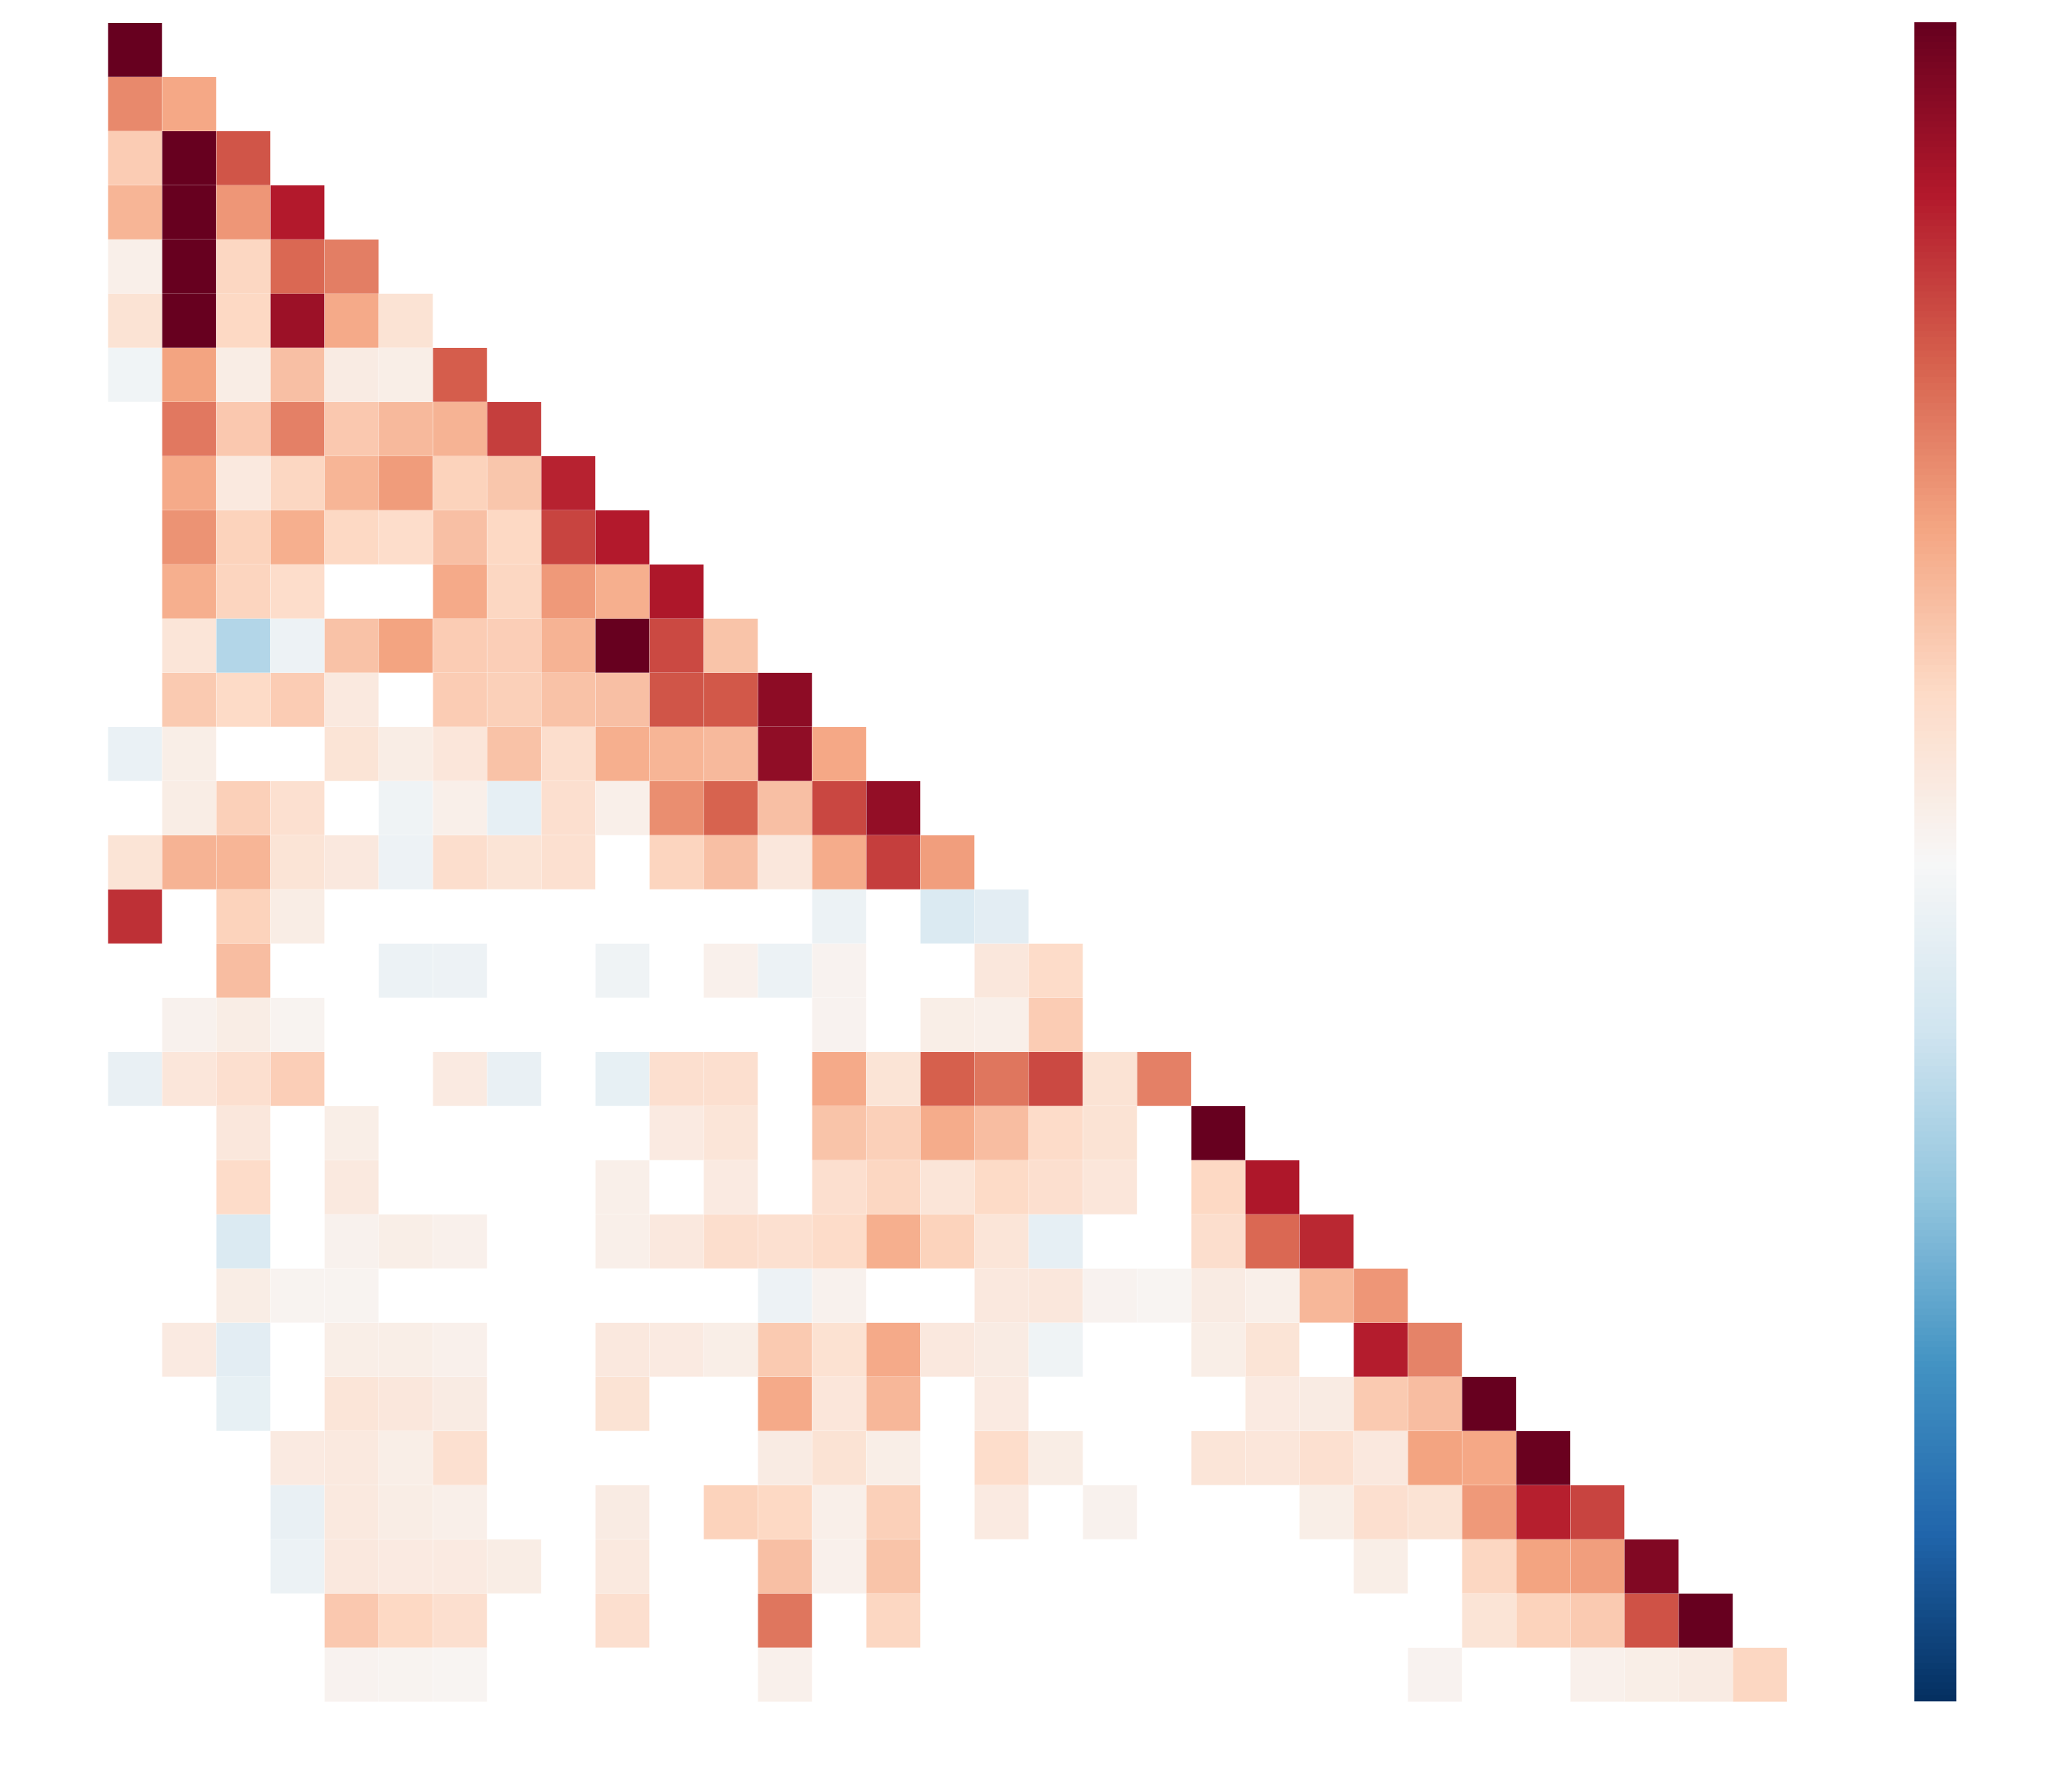
\includegraphics[width=0.62\textwidth]{./Chapter15/Figures/DLCL-picture.png}};
{\footnotesize
\node[anchor=center]  at (4.1,3){4};
\node[anchor=center]  at (4.1,1.5){2};
\node[anchor=center]  at (4.1,0){0};
\node[anchor=center]  at (4.1,-1.5){-2};
\node[anchor=center]  at (4.1,-3){-4};
\node[anchor=center]  at (-4.2,3.6){$ x_{1}$};
\node[anchor=center]  at (-4.2,2.45){$ x_{6}$};
\node[anchor=center]  at (-4.2,1.3){$ x_{11}$};
\node[anchor=center]  at (-4.2,0.15){$ x_{16}$};
\node[anchor=center]  at (-4.2,-1){$ x_{21}$};
\node[anchor=center]  at (-4.2,-2.15){$ x_{26}$};
\node[anchor=center]  at (-4.2,-3.3){$ x_{31}$};
\node[anchor=center]  at (-3.75,-3.8){$ y_{0}$};
\node[anchor=center]  at (-2.6,-3.8){$ y_{5}$};
\node[anchor=center]  at (-1.45,-3.8){$ y_{10}$};
\node[anchor=center]  at (-0.3,-3.8){$ y_{15}$};
\node[anchor=center]  at (0.85,-3.8){$ y_{20}$};
\node[anchor=center]  at (2,-3.8){$ y_{25}$};
\node[anchor=center]  at (3.15,-3.8){$ y_{30}$};
}
\end{tikzpicture}
\caption{对收敛的DLCL网络进行权重的可视化\upcite{WangLearning}}
\label{fig:15-14}
\end{figure}
%-------------------------------------------

%----------------------------------------------------------------------------------------
%    NEW SUB-SECTION
%----------------------------------------------------------------------------------------

\subsection{面向深层模型的参数初始化策略}

\parinterval 对于深层神经机器翻译模型,除了神经网络结构的设计,合适的模型参数初始化策略同样十分重要。例如,Transformer中参数矩阵采用了Xavier初始化方法\upcite{pmlr-v9-glorot10a}。该方法可以保证在训练过程中各层激活函数的输出和梯度的方差的一致性,即同时保证每层在前向和反向传播时输入和输出的方差相同。但是,这类方法更多地被用于初始化浅层神经网络,在训练深层Transformer 模型时表现不佳\upcite{pmlr-v9-glorot10a}。因此,研究人员也针对深层网络的参数初始化问题进行了探索,分为以下几种方法。

%----------------------------------------------------------------------------------------
%    NEW SUBSUB-SECTION
%----------------------------------------------------------------------------------------

\subsubsection{1. 基于深度缩放的初始化策略}

\parinterval 随着神经网络层数的加深,输入的特征要经过很多的线性及非线性变换,受神经网络中激活函数导数值域范围和连乘操作的影响,常常会带来梯度爆炸或梯度消失的问题。这个问题的原因是过多地堆叠网络层数时,无法保证反向传播过程中每层梯度方差的一致性,因此在目前深层模型中采用的很多标准化方式(如层标准化、批次标准化等)都是从方差一致性的角度来解决问题,即将各层输出的取值范围控制在激活函数的梯度敏感区域,从而维持神经网络中梯度传递的稳定性。

\parinterval 为了说明问题,首先来看一看Xavier初始化方法如何对参数矩阵$\mathbi{W}$进行初始化\upcite{pmlr-v9-glorot10a}。具体做法为从一个均匀分布中进行随机采样:
\begin{eqnarray}
\mathbi{W} & \in & \mathbb{R}^{n_i\times n_o} \sim u(-\gamma,\gamma) \\
\gamma     & = & \sqrt{\frac{6}{n_i + n_o}}
\label{eq:15-40}
\end{eqnarray}

\noindent 其中,$u(-\gamma,\gamma)$表示$-\gamma$与$\gamma$间的均匀分布,$n_i$和$n_o$分别为线性变换$\mathbi{W}$中输入和输出的维度,也就是上一层神经元的数量和下一层神经元的数量。通过这种方式可以维持在前向与反向计算过程中输入与输出方差的一致性\upcite{DBLP:conf/iccv/HeZRS15}。

\parinterval 令模型中某层神经元的输出表示为$\mathbi{Z}=\sum_{j=1}^{n_i}{w_j x_j}$。可以看出,$\mathbi{Z}$的核心是计算两个变量$w_j$和$x_j$乘积。两个变量乘积的方差的展开式为:
\begin{eqnarray}
\textrm{Var}(w_j x_j) &=& E[w_j]^2 \textrm{Var}(x_j) + E[x_j]^2 \textrm{Var}(w_j) + \textrm{Var}(w_j)\textrm{Var}(x_j)
\label{eq:15-41}
\end{eqnarray}

\parinterval 其中$\textrm{Var}(\cdot)$表示求方差操作,由于在大多数情况下,现有模型中的各种标准化方法可以维持$E[w_j]^2$和$E[x_j]^2$等于或者近似为0。因此,模型中一层神经元输出的方差可以表示为:
\begin{eqnarray}
\textrm{Var}(\mathbi{Z}) &=& \sum_{j=1}^{n_i}{\textrm{Var}(x_j) \textrm{Var}(w_j)} \nonumber \\
&=& {n_i}\textrm{Var}(\mathbi{W})\textrm{Var}(\mathbi{X})
\label{eq:15-42}
\end{eqnarray}

\parinterval 通过观察公式\eqref{eq:15-42}可以发现,在前向传播的过程中,当$\textrm{Var}(\mathbi{W})=\frac{1}{n_i}$时,可以保证每层的输入和输出的方差一致。类似的,通过相关计算可以得知,为了保证模型中每一层的输入和输出的方差一致,反向传播时应有$\textrm{Var}(\mathbi{W})=\frac{1}{n_o}$,通过对两种情况取平均值,控制参数$\mathbi{W}$的方差为$\frac{2}{n_i+n_o}$,则可以维持在前向与反向过程中输入与输出方差的一致性。若将参数初始化为一个服从边界为$[-a,b]$的均匀分布,那么其方差为$\frac{{(b+a)}^2}{12}$,为了达到$\mathbi{W}$的取值要求,初始化时应有$a=b=\sqrt{\frac{6}{n_i+n_o}}$。

\parinterval 但是随着神经网络层数的增加,上述初始化方法已经不能很好地约束基于Post-Norm的Transformer模型的输出方差。当神经网络堆叠很多层时,模型顶层输出的方差较大,同时反向传播时顶层的梯度范数也要大于底层。因此,一个自然的想法是根据网络的深度对不同层的参数矩阵采取不同的初始化方式,进而强化对各层输出方差的约束,可以描述为:
\begin{eqnarray}
\mathbi{W} & \in & \mathbb{R}^{n_i\times n_o} \sim u(-\gamma \frac{\alpha}{\sqrt{l}},\gamma \frac{\alpha}{\sqrt{l}})
\label{eq:15-43}
\end{eqnarray}

\noindent 其中,$l$为对应的神经网络的深度,$\alpha$为预先设定的超参数来控制缩放的比例。这样,可以通过缩减顶层神经网络输出与输入之间的差异,让激活函数的输入分布保持在一个稳定状态,以此来尽可能避免它们陷入梯度饱和区。

%----------------------------------------------------------------------------------------
%    NEW SUBSUB-SECTION
%----------------------------------------------------------------------------------------

\subsubsection{2. Lipschitz初始化策略}

\parinterval \ref{sec:post-pre-norm}节已经介绍,在Pre-Norm结构中每一个子层的输入为$\mathbi{x}_{l+1}^{\textrm{pre}}=\mathbi{x}_l+\mathbi{y}_l$,其中$\mathbi{x}_l$为当前子层的输入, $\mathbi{y}_l$ 为$\mathbi{x}_l$经过自注意力或前馈神经网络计算后得到的子层输出。在Post-Norm结构中,在残差连接之后还要进行层标准化操作,具体的计算流程为:

\begin{itemize}
\vspace{0.5em}
\item {\small\bfnew{计算均值}}:${\bm  \mu}=\textrm{mean}⁡(\mathbi{x}_l+\mathbi{y}_l)$
\vspace{0.5em}
\item {\small\bfnew{计算方差}}:${\bm  \sigma}=\textrm{std}⁡(\mathbi{x}_l+\mathbi{y}_l)$
\vspace{0.5em}
\item {\small\bfnew{根据均值和方差对输入进行放缩}},如下:
\begin{eqnarray}
\mathbi{x}_{l+1}^{\textrm{post}} &=& \frac{\mathbi{x}_l+\mathbi{y}_l-{\bm  \mu}}{\bm  \sigma} \cdot \mathbi{w}+\mathbi{b}
\label{eq:15-44}
\end{eqnarray}

\noindent 其中,$\mathbi{w}$和$\mathbi{b}$为可学习参数。进一步将公式\eqref{eq:15-44}展开后可得:
\begin{eqnarray}
\mathbi{x}_{l+1}^{\textrm{post}} &=& \frac{\mathbi{x}_l+\mathbi{y}_l}{\bm  \sigma} \cdot \mathbi{w} - \frac{\bm  \mu}{\bm  \sigma} \cdot \mathbi{w}+\mathbi{b} \nonumber \\
                                 &=& \frac{\mathbi{w}}{\bm  \sigma} \cdot \mathbi{x}_{l+1}^{\textrm{pre}}-\frac{\mathbi{w}}{\bm  \sigma} \cdot {\bm  \mu}+\mathbi{b}
\label{eq:15-45}
\end{eqnarray}
%\vspace{0.5em}
\end{itemize}

\parinterval 可以看到相比于Pre-Norm的计算方式,基于Post-Norm的Transformer中子层的输出为Pre-Norm形式的$\frac{\mathbi{w}}{\bm  \sigma}$倍。当$\frac{\mathbi{w}}{\bm  \sigma}<1$时,$\mathbi{x}_l$较小,输入与输出之间差异过大,导致深层Transformer系统难以收敛。Lipschitz 初始化策略通过维持条件$\frac{\mathbi{w}}{\bm  \sigma}>1$,保证网络输入与输出范数一致,进而缓解梯度消失的问题\upcite{DBLP:conf/acl/XuLGXZ20}。一般情况下,$\mathbi{w}$可以被初始化为1,因此Lipschitz 初始化方法最终的约束条件则为:
\begin{eqnarray}
0\ <\ {\bm  \sigma} &=& \textrm{std}⁡(\mathbi{x}_l+\mathbi{y}_l) \ \leq\  1
\label{eq:15-46}
\end{eqnarray}

%----------------------------------------------------------------------------------------
%    NEW SUBSUB-SECTION
%----------------------------------------------------------------------------------------

\subsubsection{3. T-Fixup初始化策略}

\parinterval 另外一种初始化方法是从神经网络结构与优化器的计算方式入手。Post-Norm结构在Warmup阶段难以精确地估计参数的二阶动量,这导致了训练不稳定问题\upcite{huang2020improving}。也就是,层标准化是导致深层Transformer难以优化的主要原因之一\upcite{WangLearning}。Post-Norm方式下Transformer的底层网络,尤其是编码器的词嵌入层面临严重的梯度消失问题。出现该问题的原因在于,在不改变层标准化位置的条件下,Adam优化器利用滑动平均的方式来估计参数的二阶矩,其方差是无界的。在训练阶段的前期,由于模型只能看到有限数量样本,因此很难有效地估计参数的二阶矩,导致反向更新参数时参数的梯度方差过大。

\parinterval 除了用Pre-Norm代替Post-Norm结构来训练深层网络,也可以采用去除Warmup策略并移除层标准化机制的方式,并对神经网络中不同的参数矩阵制定相应的缩放机制来保证训练的稳定性\upcite{huang2020improving}。具体的缩放策略如下:

\begin{itemize}
\vspace{0.5em}
\item 类似于标准的Transformer初始化方式,使用Xavier初始化方式来初始化除了词嵌入以外的所有参数矩阵。词嵌入矩阵服从$\mathbb{N}(0,d^{-\frac{1}{2}})$的高斯分布,其中$d$代表词嵌入的维度。
\vspace{0.5em}
\item 对编码器中自注意力机制的参数矩阵以及前馈神经网络中所有参数矩阵进行缩放因子为$0.67 {L}^{-\frac{1}{4}}$的缩放,$L$为编码器层数。
\vspace{0.5em}
\item 对解码器中全部注意力机制的参数矩阵以及前馈神经网络中所有参数矩阵进行缩放因子为$(9 {M})^{-\frac{1}{4}}$的缩放,其中$M$为解码器层数。
\vspace{0.5em}
\end{itemize}

\parinterval 这种初始化方法由于没有Warmup策略,学习率会直接从峰值根据参数的更新次数进行退火,大幅度增大了模型收敛的时间。因此,如何进一步解决该初始化方法下的模型收敛速度是比较关键的问题。

%----------------------------------------------------------------------------------------
%    NEW SUBSUB-SECTION
%----------------------------------------------------------------------------------------

\subsubsection{4. ADMIN初始化策略}

\parinterval 也有研究发现Post-Norm结构在训练过程中过度依赖残差支路,在训练初期很容易发生参数梯度方差过大的现象\upcite{DBLP:conf/emnlp/LiuLGCH20}。经过分析发现,虽然底层神经网络发生梯度消失是导致训练不稳定的重要因素,但并不是唯一因素。例如,标准Transformer模型中梯度消失的原因在于使用了Post-Norm结构的解码器。尽管通过调整模型结构解决了梯度消失问题,但是模型训练不稳定的问题仍然没有被很好地解决。研究人员观测到Post-Norm结构在训练过程中过于依赖残差支路,而Pre-Norm结构在训练过程中逐渐呈现出对残差支路的依赖性,这更易于网络的训练。进一步,从参数更新的角度出发,Pre-Norm由于参数的改变导致网络输出变化的方差经推导后可以表示为$O(\log L)$,而Post-Norm对应的方差为$O(L)$。因此,可以尝试减小Post-Norm中由于参数更新导致的输出的方差值,从而达到稳定训练的目的。针对该问题,可以采用两阶段的初始化方法。这里,可以重新定义子层之间的残差连接如下:
\begin{eqnarray}
\mathbi{x}_{l+1} &=& \mathbi{x}_l \cdot {\bm  \omega_{l+1}} + F_{l+1}(\mathbi{x}_l)
\label{eq:15-47}
\end{eqnarray}

\noindent 其两阶段的初始化方法如下所示:

\begin{itemize}
\vspace{0.5em}
\item {\small\bfnew{Profiling阶段}}:${\bm  \omega_{l+1}} = 1$,只进行前向计算,无需进行梯度计算。在训练样本上计算$F_{l+1}(\mathbi{x}_l)$的方差
\vspace{0.5em}
\item {\small\bfnew{Initialization阶段}}:通过Profiling阶段得到的$F_{l+1}(\mathbi{x}_l)$的方差来初始化$\bm  \omega_{l+1}$:
\begin{eqnarray}
{\bm \omega_{l+1}} &=& \sqrt{\sum_{j<l}\textrm{Var}[F_{l+1}(\mathbi{x}_l)]}
\label{eq:15-48}
\end{eqnarray}
\end{itemize}

\parinterval 这种动态的参数初始化方法不受限于具体的模型结构,有较好的通用性。

%----------------------------------------------------------------------------------------
%    NEW SUB-SECTION
%----------------------------------------------------------------------------------------

\subsection{深层模型的训练加速}

\parinterval 尽管窄而深的神经网络比宽网络有更快的收敛速度\upcite{WangLearning},但伴随着训练数据的增加,以及模型进一步的加深,训练代价成为不可忽视的问题。例如,在几千万甚至上亿的双语平行句对上训练一个48层的Transformer模型需要几周的时间才能达到收敛\footnote[5]{训练时间的估算是在单台8卡Titan V GPU服务器上得到的}。因此,在保证模型性能不变的前提下,高效地完成深层模型的训练也是至关重要的。

%----------------------------------------------------------------------------------------
%    NEW SUBSUB-SECTION
%----------------------------------------------------------------------------------------

\subsubsection{1. 渐进式训练}

\parinterval 所谓渐进式训练是指从浅层神经网络开始,在训练过程中逐渐增加模型的深度。一种比较简单的方法是将模型分为浅层部分和深层部分,之后分别进行训练,最终达到提高模型翻译性能的目的\upcite{DBLP:conf/acl/WuWXTGQLL19}。

\parinterval 另一种方式是动态构建深层模型,并尽可能复用浅层部分的训练结果\upcite{li2020shallow}。假设开始的时候模型包含$l$层神经网络,然后训练这个模型至收敛。之后,直接拷贝这$l$层神经网络(包括参数),并堆叠出一个$2l$ 层的模型。之后继续训练,重复这个过程。进行$n$次之后就得到了$(n+1) \times l$层的模型。图\ref{fig:15-15}给出了在编码器上使用渐进式训练的示意图。

%----------------------------------------------
\begin{figure}[htp]
\centering
%%%------------------------------------------------------------------------------------------------------------

\begin{center}
\begin{tikzpicture}
\begin{scope}

\node [anchor=east,fill=orange!20,draw,rounded corners=3pt,minimum height=1.6em,minimum width=1.6em] (s11) at (-0.5em, 0) {\footnotesize{$\times l$}};
\node [rectangle,anchor=west,fill=blue!20,draw,rounded corners=3pt,minimum height=1.6em,minimum width=1.6em] (s12) at ([xshift=1.2em]s11.east) {};

\node [anchor=north,fill=orange!20,draw,rounded corners=3pt,minimum height=1.6em,minimum width=1.6em] (s21) at ([yshift=-1.2em]s11.south) {\footnotesize{$\times l$}};
\node [anchor=west,fill=orange!20,draw=red,rounded corners=3pt,minimum height=1.6em,minimum width=1.6em,dashed] (s22) at ([xshift=1.2em]s21.east) {\footnotesize{$\times l$}};
\node [anchor=west,fill=blue!20,draw,rounded corners=3pt,minimum height=1.6em,minimum width=1.6em] (s23) at ([xshift=1.2em]s22.east) {};

\node [anchor=north,fill=orange!20,draw,rounded corners=3pt,minimum height=1.6em,minimum width=1.6em] (s31) at ([yshift=-1.2em]s21.south) {\footnotesize{$\times l$}};
\node [anchor=west,fill=orange!20,draw,rounded corners=3pt,minimum height=1.6em,minimum width=1.6em] (s32) at ([xshift=1.2em]s31.east) {\footnotesize{$\times l$}};
\node [anchor=west,fill=orange!20,draw=red,rounded corners=3pt,minimum height=1.6em,minimum width=1.6em,dashed] (s33) at ([xshift=1.2em]s32.east) {\footnotesize{$\times l$}};
\node [anchor=west,fill=blue!20,draw,rounded corners=3pt,minimum height=1.6em,minimum width=1.6em] (s34) at ([xshift=1.2em]s33.east) {};

\node [anchor=north,fill=orange!20,draw,rounded corners=3pt,minimum height=1.6em,minimum width=1.6em] (s41) at ([yshift=-1.2em]s31.south) {\footnotesize{$\times l$}};
\node [anchor=west,fill=orange!20,draw,rounded corners=3pt,minimum height=1.6em,minimum width=1.6em] (s42) at ([xshift=1.2em]s41.east) {\footnotesize{$\times l$}};
\node [anchor=west,fill=orange!20,draw,rounded corners=3pt,minimum height=1.6em,minimum width=1.6em] (s43) at ([xshift=1.2em]s42.east) {\footnotesize{$\times l$}};
\node [anchor=west,fill=orange!20,draw=red,rounded corners=3pt,minimum height=1.6em,minimum width=1.6em,dashed] (s44) at ([xshift=1.2em]s43.east) {\footnotesize{$\times l$}};
\node [anchor=west,fill=blue!20,draw,rounded corners=3pt,minimum height=1.6em,minimum width=1.6em] (s45) at ([xshift=1.2em]s44.east) {};

\node [anchor=east] (p1) at ([xshift=-2em]s11.west) {\footnotesize{step 1}};
\node [anchor=east] (p2) at ([xshift=-2em]s21.west) {\footnotesize{step 2}};
\node [anchor=east] (p3) at ([xshift=-2em]s31.west) {\footnotesize{step 3}};
\node [anchor=east] (p4) at ([xshift=-2em]s41.west) {\footnotesize{step 4}};

\node [anchor=south,fill=orange!20,draw,rounded corners=3pt,minimum height=1.4em,minimum width=1.4em] (b1) at ([xshift=-0.2em,yshift=1.6em]p1.north) {};
\node [anchor=west] (b2) at (b1.east) {\footnotesize{:编码器}};
\node [anchor=west,fill=blue!20,draw,rounded corners=3pt,minimum height=1.4em,minimum width=1.4em] (b3) at ([xshift=1em]b2.east) {};
\node [anchor=west] (b4) at (b3.east) {\footnotesize{:解码器}};
\node [anchor=west] (b5) at ([xshift=2em]b4.east) {\footnotesize{:拷贝}};
\draw[-latex,thick,red,dashed] ([xshift=0.5em]b4.east) -- (b5.west);

\draw [-latex, line width=0.8pt] ([xshift=-1.2em]s11.west) -- (s11.west);
\draw [-latex, line width=0.8pt] (s11.east) -- (s12.west);
\draw [-latex, line width=0.8pt] (s12.east) -- ([xshift=1.2em]s12.east);

\draw [-latex, line width=0.8pt] ([xshift=-1.2em]s21.west) -- (s21.west);
\draw [-latex, line width=0.8pt] (s21.east) -- (s22.west);
\draw [-latex, line width=0.8pt] (s22.east) -- (s23.west);
\draw [-latex, line width=0.8pt] (s23.east) -- ([xshift=1.2em]s23.east);

\draw [-latex, line width=0.8pt] ([xshift=-1.2em]s31.west) -- (s31.west);
\draw [-latex, line width=0.8pt] (s31.east) -- (s32.west);
\draw [-latex, line width=0.8pt] (s32.east) -- (s33.west);
\draw [-latex, line width=0.8pt] (s33.east) -- (s34.west);
\draw [-latex, line width=0.8pt] (s34.east) -- ([xshift=1.2em]s34.east);

\draw [-latex, line width=0.8pt] ([xshift=-1.2em]s41.west) -- (s41.west);
\draw [-latex, line width=0.8pt] (s41.east) -- (s42.west);
\draw [-latex, line width=0.8pt] (s42.east) -- (s43.west);
\draw [-latex, line width=0.8pt] (s43.east) -- (s44.west);
\draw [-latex, line width=0.8pt] (s44.east) -- (s45.west);
\draw [-latex, line width=0.8pt] (s45.east) -- ([xshift=1.2em]s45.east);

\draw[-latex,thick,red,dashed] (s11.south)..controls +(south:1em) and +(north:1.2em)..(s22.north);
\draw[-latex,thick,red,dashed] (s22.south)..controls +(south:1em) and +(north:1.2em)..(s33.north);
\draw[-latex,thick,red,dashed] (s33.south)..controls +(south:1em) and +(north:1.2em)..(s44.north);
\end{scope} 
\end{tikzpicture}
\end{center}



\caption{渐进式深层模型训练过程}
\label{fig:15-15}
\end{figure}
%-------------------------------------------

\parinterval 渐进式训练的好处在于深层模型并不是从头开始训练。每一次堆叠,都相当于利用“浅”模型给“深”模型提供了一个很好的初始点,这样深层模型的训练会更加容易。

%----------------------------------------------------------------------------------------
%    NEW SUBSUB-SECTION
%----------------------------------------------------------------------------------------

\subsubsection{2. 分组稠密连接}

\parinterval 很多研究工作已经发现深层模型不同层之间的稠密连接能够很明显地提高信息传递的效率\upcite{WangLearning,DBLP:conf/cvpr/HuangLMW17,Dou2018ExploitingDR,DBLP:conf/acl/WuWXTGQLL19}。与此同时,对之前层信息的不断复用有助于得到更好的表示,但也带来了计算代价过大的问题。在动态线性层聚合方法(DLCL)中,每一次聚合时都需要重新计算之前每一层表示对当前层输入的贡献度,因此伴随着编码器整体深度的增加,这部分的计算代价变得不可忽略。例如,一个基于动态层聚合的48层Transformer模型比不使用动态层聚合的模型在进行训练时慢近2倍。同时,缓存中间结果也增加了显存的使用量。比如,即使在使用半精度计算的情况下,每张12G显存的GPU上计算的词也不能超过2048个,这导致训练开销急剧增大。

%----------------------------------------------
\begin{figure}[htp]
\centering
%%%------------------------------------------------------------------------------------------------------------
\begin{center}
\begin{tikzpicture}
\begin{scope}

\node [anchor=east,fill=orange!20,draw,rounded corners=3pt,minimum height=1.4em,minimum width=1.4em] (s11) at (-0.5em, 0) {};
\node [rectangle,anchor=west,fill=orange!20,draw,rounded corners=3pt,minimum height=1.4em,minimum width=1.4em] (s12) at ([xshift=2em]s11.east) {};
\node [anchor=west,fill=orange!20,draw,rounded corners=3pt,minimum height=1.4em,minimum width=1.4em] (s13) at ([xshift=2em]s12.east) {};
\node [anchor=west,fill=orange!20,draw,rounded corners=3pt,minimum height=1.4em,minimum width=1.4em] (s14) at ([xshift=2em]s13.east) {};

\node [anchor=north,fill=orange!20,draw,rounded corners=3pt,minimum height=1.4em,minimum width=1.4em] (s21) at ([yshift=-2.5em]s11.south) {};
\node [anchor=west,fill=orange!20,draw,rounded corners=3pt,minimum height=1.4em,minimum width=1.4em] (s22) at ([xshift=2em]s21.east) {};
\node [anchor=west,fill=orange!20,draw,rounded corners=3pt,minimum height=1.4em,minimum width=1.4em] (s23) at ([xshift=2em]s22.east) {};
\node [anchor=west,fill=orange!20,draw,rounded corners=3pt,minimum height=1.4em,minimum width=1.4em] (s24) at ([xshift=2em]s23.east) {};

\node [anchor=north,fill=orange!20,draw,rounded corners=3pt,minimum height=1.4em,minimum width=1.4em] (s31) at ([yshift=-2.5em]s21.south) {};
\node [anchor=west,fill=orange!20,draw,rounded corners=3pt,minimum height=1.4em,minimum width=1.4em] (s32) at ([xshift=2em]s31.east) {};
\node [anchor=west,fill=orange!20,draw,rounded corners=3pt,minimum height=1.4em,minimum width=1.4em] (s33) at ([xshift=2em]s32.east) {};
\node [anchor=west,fill=orange!20,draw,rounded corners=3pt,minimum height=1.4em,minimum width=1.4em] (s34) at ([xshift=2em]s33.east) {};

\node [anchor=north,fill=orange!20,draw,rounded corners=3pt,minimum height=1.4em,minimum width=1.4em] (s41) at ([yshift=-2.5em]s31.south) {};
\node [anchor=west,fill=orange!20,draw,rounded corners=3pt,minimum height=1.4em,minimum width=1.4em] (s42) at ([xshift=2em]s41.east) {};
\node [anchor=west,fill=orange!20,draw,rounded corners=3pt,minimum height=1.4em,minimum width=1.4em] (s43) at ([xshift=2em]s42.east) {};
\node [anchor=west,fill=orange!20,draw,rounded corners=3pt,minimum height=1.4em,minimum width=1.4em] (s44) at ([xshift=2em]s43.east) {};

\node [anchor=east] (p1) at ([xshift=-3.5em]s11.west) {$p=\infty$};
\node [anchor=east] (p2) at ([xshift=-4em]s21.west) {$p=1$};
\node [anchor=east] (p3) at ([xshift=-4em]s31.west) {$p=2$};
\node [anchor=east] (p4) at ([xshift=-4em]s41.west) {$p=4$};
\node [anchor=north] (p5) at ([yshift=-1em]p3.south) {$\cdots$};
\node [anchor=south,fill=orange!20,draw,rounded corners=3pt,minimum height=1.4em,minimum width=1.4em] (b1) at ([xshift=-0.6em,yshift=1.2em]p1.north) {};
\node [anchor=west] (b2) at (b1.east) {\footnotesize{:Layer}};
\node [anchor=west,draw=red,rounded corners=3pt,minimum height=1.4em,minimum width=1.4em,dashed,line width=0.8pt] (b3) at ([xshift=1em]b2.east) {};
\node [anchor=west] (b4) at (b3.east) {\footnotesize{:Block}};

\draw [-latex, line width=0.8pt] ([xshift=-2em]s11.west) -- (s11.west);
\draw [-latex, line width=0.8pt] (s11.east) -- (s12.west);
\draw [-latex, line width=0.8pt] (s12.east) -- (s13.west);
\draw [-latex, line width=0.8pt] (s13.east) -- (s14.west);
\draw [-latex, line width=0.8pt] (s14.east) -- ([xshift=2em]s14.east);

\draw [-latex, line width=0.8pt] ([xshift=-2em]s21.west) -- (s21.west);
\draw [-latex, line width=0.8pt] (s21.east) -- (s22.west);
\draw [-latex, line width=0.8pt] (s22.east) -- (s23.west);
\draw [-latex, line width=0.8pt] (s23.east) -- (s24.west);
\draw [-latex, line width=0.8pt] (s24.east) -- ([xshift=2em]s24.east);

\draw [-latex, line width=0.8pt] ([xshift=-2em]s31.west) -- (s31.west);
\draw [-latex, line width=0.8pt] (s31.east) -- (s32.west);
\draw [-latex, line width=0.8pt] (s32.east) -- (s33.west);
\draw [-latex, line width=0.8pt] (s33.east) -- (s34.west);
\draw [-latex, line width=0.8pt] (s34.east) -- ([xshift=2em]s34.east);

\draw [-latex, line width=0.8pt] ([xshift=-2em]s41.west) -- (s41.west);
\draw [-latex, line width=0.8pt] (s41.east) -- (s42.west);
\draw [-latex, line width=0.8pt] (s42.east) -- (s43.west);
\draw [-latex, line width=0.8pt] (s43.east) -- (s44.west);
\draw [-latex, line width=0.8pt] (s44.east) -- ([xshift=2em]s44.east);


\node [draw=red,rounded corners=3pt,minimum height=1.7em,minimum width=1.7em,dashed,line width=0.8pt] (x21) at (s21) {};
\node [draw=red,rounded corners=3pt,minimum height=1.7em,minimum width=1.7em,dashed,line width=0.8pt] (x22) at (s22) {};
\node [draw=red,rounded corners=3pt,minimum height=1.7em,minimum width=1.7em,dashed,line width=0.8pt] (x23) at (s23) {};
\node [draw=red,rounded corners=3pt,minimum height=1.7em,minimum width=1.7em,dashed,line width=0.8pt] (x24) at (s24) {};

\node [draw=red,rounded corners=3pt,minimum height=1.7em,minimum width=5.2em,dashed,line width=0.8pt] (x31) at ([xshift=1.75em]s31) {};
\node [draw=red,rounded corners=3pt,minimum height=1.7em,minimum width=5.2em,dashed,line width=0.8pt] (x32) at ([xshift=1.75em]s33) {};

\node [draw=red,rounded corners=3pt,minimum height=1.7em,minimum width=12.2em,dashed,line width=0.8pt] (x41) at ([xshift=1.75em]s42) {};

{
\draw [-latex, line width=0.8pt] ([xshift=-1em]s21.west).. controls +(58:0.6) and +(122:0.6) .. ([xshift=1em]s21.east);
\draw [-latex, line width=0.8pt] ([xshift=-1em]s22.west).. controls +(58:0.6) and +(122:0.6) .. ([xshift=1em]s22.east);
\draw [-latex, line width=0.8pt] ([xshift=-1em]s23.west).. controls +(58:0.6) and +(122:0.6) .. ([xshift=1em]s23.east);
\draw [-latex, line width=0.8pt] ([xshift=-1em]s24.west).. controls +(58:0.6) and +(122:0.6) .. ([xshift=1em]s24.east);
}

{
\draw [-latex, line width=0.8pt] ([xshift=-1em]s21.west).. controls +(65:0.8) and +(115:0.8) .. ([xshift=1em]s22.east);
\draw [-latex, line width=0.8pt] ([xshift=-1em]s22.west).. controls +(65:0.8) and +(115:0.8) .. ([xshift=1em]s23.east);
\draw [-latex, line width=0.8pt] ([xshift=-1em]s23.west).. controls +(65:0.8) and +(115:0.8) .. ([xshift=1em]s24.east);
\draw [-latex, line width=0.8pt] ([xshift=-1em]s31.west).. controls +(65:0.8) and +(115:0.8) .. ([xshift=1em]s32.east);
\draw [-latex, line width=0.8pt] ([xshift=-1em]s33.west).. controls +(65:0.8) and +(115:0.8) .. ([xshift=1em]s34.east);
}

{
\draw [-latex, line width=0.8pt] ([xshift=-1em]s21.west).. controls +(70:1.0) and +(110:1.0) .. ([xshift=1em]s23.east);
\draw [-latex, line width=0.8pt] ([xshift=-1em]s22.west).. controls +(70:1.0) and +(110:1.0) .. ([xshift=1em]s24.east);
}

{
\draw [-latex, line width=0.8pt] ([xshift=-1em]s21.west).. controls +(75:1.2) and +(105:1.2) .. ([xshift=1em]s24.east);
\draw [-latex, line width=0.8pt] ([xshift=-1em]s31.west).. controls +(75:1.2) and +(105:1.2) .. ([xshift=1em]s34.east);
\draw [-latex, line width=0.8pt] ([xshift=-1em]s41.west).. controls +(75:1.2) and +(105:1.2) .. ([xshift=1em]s44.east);
}
\end{scope} 
\end{tikzpicture}
\end{center}



\caption{不同组之间的稀疏连接}
\label{fig:15-16}
\end{figure}
%-------------------------------------------

\parinterval 缓解这个问题的一种方法是使用更稀疏的层间连接方式。其核心思想与动态线性层聚合是类似的,不同点在于可以通过调整层之间连接的稠密程度来降低训练代价。比如,可以将每$p$层分为一组,之后动态线性层聚合只在不同组之间进行。这样,通过调节$p$值的大小可以控制神经网络中连接的稠密程度,作为一种训练代价与翻译性能之间的权衡。显然,标准的Transformer模型\upcite{vaswani2017attention} 和DLCL模型\upcite{WangLearning}都可以看作是该方法的一种特例。如图\ref{fig:15-16}所示:当$p=1$时,每一个单独的块被看作一个独立的组,它等价于基于动态层聚合的DLCL模型;当$p=\infty$时,它等价于正常的Transformer模型。值得注意的是,如果配合渐进式训练。在分组稠密连接中可以设置$p$等于模型层数。

%----------------------------------------------------------------------------------------
%    NEW SUBSUB-SECTION
%----------------------------------------------------------------------------------------

\subsubsection{3. 学习率重置}

\parinterval 尽管渐进式训练策略与分组稠密连接结构都可以加速深层模型的训练,但使用传统的学习率衰减策略会导致训练深层模型时的学习率较小,因此模型无法快速地达到收敛状态,同时也影响最终的模型性能。

\parinterval  图\ref{fig:15-17}中的红色曲线描绘了在WMT英德翻译任务上标准Transformer模型的学习率曲线,可以看到当模型训练到40k步时,学习率对比峰值有明显的差距,而此时刚开始训练最终的深层模型,过小的学习率并不利于后期深层网络的充分训练。

%----------------------------------------------
\begin{figure}[htp]
\centering
\begin{center}
  \begin{tikzpicture}[scale=1.0]
    \footnotesize{
      \begin{axis}[
      width=.50\textwidth,
      height=.40\textwidth,
      legend style={at={(0.45,0.08)}, anchor=south west},
      xlabel={\scriptsize{更新次数(10k)}},
      ylabel={\scriptsize{学习率 ($10^{-3}$)}},
      ylabel style={yshift=-1em},xlabel style={yshift=0.0em},
      yticklabel style={/pgf/number format/precision=2,/pgf/number format/fixed zerofill},
      ymin=0,ymax=2.2, ytick={0.5, 1, 1.5, 2},
      xmin=0,xmax=5,xtick={1,2,3,4},
      legend style={xshift=-8pt,yshift=-4pt, legend plot pos=right,font=\scriptsize,cells={anchor=west}}
      ]

      \addplot[red,line width=1.25pt] coordinates {(0,0) (1.6,2) (1.8,1.888) (2,1.787) (2.5,1.606) (3,1.462) (3.5,1.3549) (4,1.266) (4.5,1.193) (5,1.131)};
      \addlegendentry{\scriptsize 原始的学习率}
      %\addplot[red,line width=1.25pt] coordinates {(0,0) (8000,0.002) (10000,0.00179) (12000,0.00163) (12950,0.001572)};
      \addplot[blue,line width=1.25pt] coordinates {(0,0) (0.8,2) (0.9906,1.7983)};
      %\addplot[red,line width=1.25pt] coordinates {(0,0) (8000,0.002) (9906,0.0017983)};
      \addplot[blue,dashed,line width=1.25pt] coordinates {(0.9906,1.7983) (0.9906,2)};
      \addplot[blue,line width=1.25pt] coordinates {(0.9906,2) (1.1906,1.79) (1.3906,1.63) (1.4856,1.572)};
      \addplot[blue,dashed,line width=1.25pt] coordinates {(1.4856,1.572) (1.4856,2)};
      \addplot[blue,line width=1.25pt] coordinates {(1.4856,2) (1.6856,1.79) (1.8856,1.63) (1.9806,1.572)};
      \addplot[blue,dashed,line width=1.25pt] coordinates {(1.9806,1.572) (1.9806,2)};
      \addplot[blue,line width=1.25pt] coordinates {(1.9806,2) (2.1806,1.79) (2.3806,1.63) (2.4756,1.572)};
      \addplot[blue,dashed,line width=1.25pt] coordinates {(2.4756,1.572) (2.4756,2)};
      \addplot[blue,line width=1.25pt] coordinates {(2.4756,2) (2.6756,1.79) (2.8756,1.63) (2.9706,1.572)};
      \addplot[blue,dashed,line width=1.25pt] coordinates {(2.9706,1.572) (2.9706,2)};
      \addplot[blue,line width=1.25pt] coordinates {(2.9706,2) (3.1706,1.79) (3.3706,1.63) (3.4656,1.572) (3.6706,1.4602) (3.7136,1.44)};
      \addplot[blue,dashed,line width=1.25pt] coordinates {(3.7136,1.44) (3.7136,2)};
      \addplot[blue,line width=1.25pt] coordinates {(3.7136,2) (3.9136,1.79) (4.1136,1.63) (4.2086,1.572) (4.4136,1.4602) (4.4566,1.44) (4.7000,1.3574) (5.0000,1.2531)};
      \addlegendentry{\scriptsize 重置后的学习率}

      \end{axis}
     }
  \end{tikzpicture}
\end{center}
\caption{学习率重置vs从头训练的学习率曲线}
\label{fig:15-17}
\end{figure}
%-------------------------------------------

\parinterval 针对该问题的一个解决方案是修改学习率曲线的衰减策略,如图\ref{fig:15-17}所示。图中蓝色的曲线是修改后的学习率曲线。首先在训练的初期让模型快速地达到学习率的峰值(线性递增),之后的每一次增加$l$层神经网络时,都会将当前的学习率值重置到峰值点。之后,根据训练的步数对其进行相应的衰减。具体的步骤如下:

\begin{itemize}
\vspace{0.5em}
\item 在训练的初期,模型会先经历一个学习率预热的过程:
\begin{eqnarray}
lr &=& d_{\textrm{model}}^{-0.5}\cdot step\_num \cdot warmup\_steps^{-0.5}
\label{eq:15-49}
\end{eqnarray}
\noindent 这里,$step\_num$表示参数更新的次数,$warmup\_step$表示预热的更新次数,$d_{\textrm{model}}$表示Transformer模型的隐层大小,$lr$是学习率。
\vspace{0.5em}
\item 	在之后的训练过程中,每当增加模型深度时,学习率都会重置到峰值,之后进行相应的衰减:
\begin{eqnarray}
lr &=& d_{\textrm{model}}^{-0.5}\cdot step\_num^{-0.5}
\label{eq:15-50}
\end{eqnarray}
\noindent 这里$step\_num$代表学习率重置后更新的步数。
\vspace{0.5em}
\end{itemize}

\parinterval 综合使用渐进式训练、分组稠密连接、学习率重置策略可以保证在翻译品质不变的前提下,缩减近$40\%$的训练时间\upcite{li2020shallow}。同时,伴随着模型的加深与数据集的增大加速比也会进一步地增大。

%----------------------------------------------------------------------------------------
%    NEW SUB-SECTION
%----------------------------------------------------------------------------------------

\subsection{深层模型的健壮性训练}


\parinterval 伴随着网络的加深,模型的训练还会面临另外一个比较严峻的问题\ \dash \ 过拟合。由于参数量的增大,深层模型的输入与输出分布之间的差异也会越来越大,然而不同子层之间的相互适应也会更加的明显,这将导致任意子层网络对其他子层的依赖过大。这种现象在训练阶段是有帮助的,因为不同子层可以协同工作从而更好地拟合训练数据。然而这种方式也降低了模型的泛化能力,即深层模型更容易陷入过拟合问题。

\parinterval 通常,可以使用Dropout手段用来缓解过拟合问题(见{\chapterthirteen})。不幸的是,尽管目前Transformer模型使用了多种Dropout手段(如Residual Dropout、Attention Dropout、 ReLU Dropout等),过拟合问题在深层模型中仍然存在。从图\ref{fig:15-18}中可以看到,深层模型比浅层模型在训练集和校验集的困惑度上都有明显的优势,然而模型在训练一段时间后出现校验集困惑度上涨的现象,说明模型已经过拟合于训练数据。

%----------------------------------------------
\begin{figure}[htp]
\centering
\definecolor{ublue}{rgb}{0.152,0.250,0.545}
\begin{tikzpicture}
\begin{axis}
[  
  width=5cm, height=3.5cm, 
  xtick={15,17,19,21,23,25},
  ytick={6.0,6.5,7.0},
  xlabel={\scriptsize Epoch},
  ylabel={},
  ylabel style={},
  x tick label style={},
  y tick label style={},
  tick align=inside,
  legend style={anchor=north,xshift=1.7cm,yshift=1cm,legend  columns =-1},
  ymin=5.7,
  ymax=7.3,
  xmin=14.6,
  xmax=25.4,
  extra y ticks={6.0,6.5,7.0},
  extra y tick labels={3.7,3.8,3.9},
  extra y tick style={ticklabel pos=right}]
  \addplot [sharp plot,very thick,red!60,mark=diamond*] coordinates{(15,6.75) (16,6.73) (17,6.70) (18,6.67) (19,6.64) (20,6.61) (21,6.59) (22,6.58) (23,6.57) (24,6.58) (25,6.59)};
  \addplot [sharp plot,very thick,purple!60,mark=triangle*] coordinates{(15,6.70) (16,6.4) (17,6.20) (18,6.30) (19,6.20) (20,6.10) (21,6.15) (22,6.10) (23,6.15) (24,6.16) (25,6.17)};
  \legend{\scriptsize {训练集},\scriptsize{校验集}}
\end{axis}
\begin{axis}
[ xshift=6.6cm,
  width=5cm, height=3.5cm, 
  xtick={15,17,19,21,23,25},
  ytick={5.0,5.5,6.0},
  xlabel={\scriptsize Epoch},
  ylabel={},
  ylabel style={},
  x tick label style={},
  y tick label style={},
  tick align=inside,
  ymin=4.7,
  ymax=6.3,
  xmin=14.6,
  xmax=25.4,
  extra y ticks={5.0,5.5,6.0},
  extra y tick labels={3.5,3.6,3.7},
  extra y tick style={ticklabel pos=right}]
  \addplot [sharp plot,very thick,red!60,mark=diamond*] coordinates{(15,5.7) (16,5.65) (17,5.6) (18,5.55) (19,5.5) (20,5.45) (21,5.4) (22,5.38) (23,5.36) (24,5.34) (25,5.27)};
  \addplot [sharp plot,very thick,purple!60,mark=triangle*] coordinates{(15,5.0) (16,4.9) (17,4.9) (18,5.05) (19,4.9) (20,5.0) (21,5.0) (22,5.1) (23,5.0) (24,5.15) (25,5.5)};
\end{axis}
\node [anchor=north,rotate=90] (n1) at (-1.3cm,1cm) {\scriptsize 训练集\ PPL};
\node [anchor=north,rotate=90] (n2) at (5.4cm,1cm) {\scriptsize 训练集\ PPL};
\node [anchor=north,rotate=90] (n3) at (4.2cm,1cm) {\scriptsize 校验集\ PPL};
\node [anchor=north,rotate=90] (n4) at (10.7cm,1cm) {\scriptsize 校验集\ PPL};
\end{tikzpicture}

%---------------------------------------------------------------------
\caption{浅层模型(左)与深层模型(右)在WMT16英德翻译任务的校验集与训练集的困惑度}
\label{fig:15-18}
\end{figure}
%-------------------------------------------

\parinterval {\chapterthirteen}提到的Layer Dropout方法可以有效地缓解这个问题。以编码器为例, Layer Dropout的过程可以被描述为:在训练过程中,对自注意力子层或前馈神经网络子层进行随机丢弃,以减少不同子层之间的相互适应。这里选择Pre-Norm结构作为基础架构,它可以被描述为:
\begin{eqnarray}
\mathbi{x}_{l+1} &=& F(\textrm{LN}(\mathbi{x}_l)) + \mathbi{x}_l
\label{eq:15-51}
\end{eqnarray}

\noindent 其中,$\textrm{LN}( \cdot )$表示层标准化函数, $F( \cdot )$表示自注意力机制或者前馈神经网络,$\mathbi{x}_l$表示第$l$个子层的输入。之后,使用一个掩码$\textrm{Mask}$(值为0或1)来控制每个子层是正常计算还是丢弃。于是,该子层的计算公式可以被重写为:
\begin{eqnarray}
\mathbi{x}_{l+1} &=& \textrm{Mask} \cdot F(\textrm{LN}(\mathbi{x}_l))+\mathbi{x}_l
\label{eq:15-52}
\end{eqnarray}

\noindent $\textrm{Mask}=0$代表该子层被丢弃,而$\textrm{Mask}=1$代表正常进行当前子层的计算。图\ref{fig:15-19}展示了这个方法与标准Pre-Norm结构之间的区别。

%----------------------------------------------
\begin{figure}[htp]
\centering
%%%------------------------------------------------------------------------------------------------------------
%%% 调序模型1:基于距离的调序
\begin{center}
\begin{tikzpicture}

\begin{scope}[minimum height = 20pt]

\node [anchor=east] (x1) at (-0.5em, 0) {$\mathbi{x}_l$};
\node [anchor=west,draw,fill=red!30,inner xsep=5pt,rounded corners=2pt,draw,thick] (ln1) at ([xshift=1em]x1.east){\small{\textrm{LN}}};
\node [anchor=west,draw,fill=green!30,inner xsep=5pt,rounded corners=2pt,draw,thick] (f1) at ([xshift=0.6em]ln1.east){\small{$F$}};
\node [anchor=west,circle,draw,,minimum size=1em,thick] (n1) at ([xshift=3em]f1.east){};
\node [anchor=west] (x2) at ([xshift=1em]n1.east) {$\mathbi{x}_{l+1}$};
\node [anchor=west,draw,fill=red!30,inner xsep=5pt,rounded corners=2pt,draw,thick] (ln12) at ([xshift=1em]x2.east){\small{\textrm{LN}}};
\node [anchor=west,draw,fill=green!30,inner xsep=5pt,rounded corners=2pt,draw,thick] (f12) at ([xshift=0.6em]ln12.east){\small{$F$}};
\node [anchor=west,circle,draw,,minimum size=1em,thick] (n12) at ([xshift=3em]f12.east){};
\node [anchor=west] (x22) at ([xshift=1em]n12.east) {$\mathbi{x}_{l+2}$};

\node [anchor=north] (x3) at ([yshift=-5em]x1.south) {$\mathbi{x}_l$};
\node [anchor=west,draw,fill=red!30,inner xsep=5pt,rounded corners=2pt,draw,thick] (ln2) at ([xshift=1em]x3.east){\small{\textrm{LN}}};
\node [anchor=west,draw,fill=green!30,inner xsep=5pt,rounded corners=2pt,draw,thick] (f2) at ([xshift=0.6em]ln2.east){\small{$F$}};
\node [anchor=west,minimum size=1em] (p1) at ([xshift=1em]f2.east){};
\node [anchor=north] (m1) at ([yshift=0.6em]p1.south){\footnotesize{\red{Mask=1}}};
\node [anchor=west,circle,draw,,minimum size=1em,thick] (n2) at ([xshift=3em]f2.east){};
\node [anchor=west] (x4) at ([xshift=1em]n2.east) {$\mathbi{x}_{l+1}$};
\node [anchor=west,draw,fill=red!30,inner xsep=5pt,rounded corners=2pt,draw,thick] (ln22) at ([xshift=1em]x4.east){\small{\textrm{LN}}};
\node [anchor=west,draw,fill=green!30,inner xsep=5pt,rounded corners=2pt,draw,thick] (f22) at ([xshift=0.6em]ln22.east){\small{$F$}};
\node [anchor=west,minimum size=1em] (p2) at ([xshift=1em]f22.east){};
\node [anchor=north] (m2) at ([yshift=0.6em]p2.south){\footnotesize{\red{Mask=0}}};
\node [anchor=west,circle,draw,,minimum size=1em,thick] (n22) at ([xshift=3em]f22.east){};
\node [anchor=west] (x42) at ([xshift=1em]n22.east) {$\mathbi{x}_{l+2}$};

\draw[->, line width=1pt] ([xshift=-0.1em]x1.east)--(ln1.west);
\draw[->, line width=1pt] ([xshift=-0.1em]ln1.east)--(f1.west);
\draw[->, line width=1pt] ([xshift=0.1em]f1.east)--(n1.west);
\draw[->, line width=1pt] (n1.east)--(x2.west);
\draw[->, line width=1pt] ([xshift=-0.1em]x3.east)--(ln2.west);
\draw[->, line width=1pt] ([xshift=-0.1em]ln2.east)--(f2.west);
\draw[-, line width=1pt] ([xshift=0.1em]f2.east)--(p1.west);
\draw[*-,red,line width=0.6pt] (p1.west) -- (p1.east);
\draw[->, line width=1pt] (p1.east)--(n2.west);
\draw[->, line width=1pt] (n2.east)--(x4.west);
\draw[->,rounded corners,line width=1pt] ([yshift=-0.2em]x1.north) -- ([yshift=1em]x1.north) -- ([yshift=1.4em]n1.north) -- (n1.north);
\draw[->,rounded corners,line width=1pt] ([yshift=-0.2em]x3.north) -- ([yshift=1em]x3.north) -- ([yshift=1.4em]n2.north) -- (n2.north);
\draw[-,thick] (n1.west)--(n1.east);
\draw[-,thick] (n1.north)--(n1.south);
\draw[-,thick] (n2.west)--(n2.east);
\draw[-,thick] (n2.north)--(n2.south);

\draw[->, line width=1pt] ([xshift=-0.1em]x2.east)--(ln12.west);
\draw[->, line width=1pt] ([xshift=-0.1em]ln12.east)--(f12.west);
\draw[->, line width=1pt] ([xshift=0.1em]f12.east)--(n12.west);
\draw[->, line width=1pt] (n12.east)--(x22.west);
\draw[->, line width=1pt] ([xshift=-0.1em]x4.east)--(ln22.west);
\draw[->, line width=1pt] ([xshift=-0.1em]ln22.east)--(f22.west);
\draw[-, line width=1pt] ([xshift=0.1em]f22.east)--(p2.west);
\draw[*-,red,line width=0.6pt] ([yshift=-0.1em]p2.west) -- (p2.north east);
\draw[->, line width=1pt] (p2.east)--(n22.west);
\draw[->, line width=1pt] (n22.east)--(x42.west);
\draw[->,rounded corners,line width=1pt] ([yshift=-0.2em]x2.north) -- ([yshift=1em]x2.north) -- ([yshift=1.4em]n12.north) -- (n12.north);
\draw[->,rounded corners,line width=1pt] ([yshift=-0.2em]x4.north) -- ([yshift=1em]x4.north) -- ([yshift=1.4em]n22.north) -- (n22.north);
\draw[-,thick] (n12.west)--(n12.east);
\draw[-,thick] (n12.north)--(n12.south);
\draw[-,thick] (n22.west)--(n22.east);
\draw[-,thick] (n22.north)--(n22.south);

\node [anchor=south] (k1) at ([yshift=-0.1em]x1.north){};
\node [anchor=south] (k2) at ([yshift=-0.1em]x3.north){};
\begin{pgfonlayer}{background}
\node [rectangle,inner sep=0.3em,fill=orange!10] [fit = (x1) (f1) (n1) (ln1) (x2) (k1) (f12) (n12) (ln12) (x22)] (box0) {};
\node [rectangle,inner sep=0.3em,fill=blue!10] [fit = (x3) (f2) (n2) (ln2) (x4) (k2) (f22) (n22) (ln22) (x42)] (box1) {};
\end{pgfonlayer}

\node [anchor=north] (c1) at (box0.south){\footnotesize {(a)标准的Pre-Norm}};
\node [anchor=north] (c2) at (box1.south){\footnotesize {(b)基于随机子层跳跃的Pre-Norm}};
\end{scope}
\end{tikzpicture}
\end{center}
\caption{标准的Pre-Norm结构与基于随机子层跳跃的Pre-Norm结构}
\label{fig:15-19}
\end{figure}
%-------------------------------------------

\parinterval 除此之外,在残差网络中,研究人员已经发现底层神经网络的作用是对输入进行抽象表示,而上层神经网络会进一步修正这种表示来拟合训练目标,因此底层神经网络对模型最终的输出有很大的影响\upcite{DBLP:journals/corr/GreffSS16}。该结论同样适用于Transformer模型,比如,在训练中,残差支路以及底层的梯度范数通常比较大,这也间接表明底层神经网络在整个优化的过程中需要更大的更新。考虑到这个因素,在设计每一个子层被丢弃的概率时,可以采用自底向上线性增大的策略,保证底层的神经网络相比于顶层更容易保留下来。

%----------------------------------------------------------------------------------------
%    NEW SECTION
%----------------------------------------------------------------------------------------

\sectionnewpage
\section{基于句法的神经机器翻译模型}

\parinterval 在统计机器翻译时代,使用句法信息是一种非常有效的机器翻译建模手段(见{\chaptereight})。由于句法是人类运用语言的高级抽象结果,使用句法信息(如句法树)可以帮助机器翻译系统对句子结构进行建模。例如,利用句法树提升译文语法结构的正确性。在神经机器翻译中,大多数框架均基于词串进行建模,因此在模型中引入句法树等结构也很有潜力\upcite{DBLP:conf/acl/LiXTZZZ17}。 具体来说,由于传统神经机器翻译模型缺少对句子结构的理解,会导致一些翻译问题:

\begin{itemize}
\vspace{0.5em}
\item {\small\bfnew{过度翻译问题}},如:
\begin{equation}
\textrm{“ 两/个/女孩 ”}\ \to \ \textrm{“ two girls and two girls ”} \nonumber
\end{equation}

\vspace{0.5em}
\item {\small\bfnew{翻译不连贯问题}},如:
\begin{equation}
\textrm{“ 新生/银行/申请/上市 ”}\ \to \ \textrm{“ new listing bank ”} \nonumber
\end{equation}

\vspace{0.5em}
\end{itemize}

\parinterval 显然,神经机器翻译系统并没有按照合理的句法结构生成译文。也就是说,模型并没有理解句子的结构\upcite{DBLP:conf/acl/LiXTZZZ17}。甚至对于一些语言差异很大的语言对,会出现将介词短语翻译成一个词的情况。虽然可以通过很多手段对上述问题进行求解,但是使用句法树是解决该问题的一种最直接的方法\upcite{DBLP:conf/acl/EriguchiHT16}。

\parinterval 那么在神经机器翻译中,如何将这种离散化的树结构融入到基于分布式表示的翻译模型中呢?有以下两种策略:

\begin{itemize}
\vspace{0.5em}
\item {\small\bfnew{将句法信息加入到编码器}},使得编码器更加充分地表示源语言句子。
\vspace{0.5em}
\item {\small\bfnew{将句法信息加入到解码器}},使得翻译模型能生成更符合句法的译文。
\vspace{0.5em}
\end{itemize}

%----------------------------------------------------------------------------------------
%    NEW SUB-SECTION
%----------------------------------------------------------------------------------------

\subsection{编码器使用句法信息}

\parinterval 在编码器中使用句法信息有两种思路,一种思路是在编码器中显性使用树结构进行建模,另一种思路是把句法信息作为特征输入到传统的序列编码器中。这两种思路与统计机器翻译中基于句法树结构的模型和基于句法特征的模型十分相似(见{\chaptereight})。

%----------------------------------------------------------------------------------------
%    NEW SUBSUB-SECTION
%----------------------------------------------------------------------------------------

\subsubsection{1. 基于句法树结构的编码}

\parinterval 使用句法信息的一种简单的方法是将源语言句子编码成一个二叉树结构\footnote[6]{所有句法树都可以通过二叉化方法转化为二叉树(见{\chaptereight})。},树节点的信息是由左子树和右子树变换而来,如下所示:
\begin{eqnarray}
\mathbi{h}_p &=& f_\textrm{tree}(\mathbi{h}_l,\mathbi{h}_r)
\label{eq:15-53}
\end{eqnarray}

\noindent 其中,$\mathbi{h}_l$和$\mathbi{h}_r$分别代表了左孩子节点和右孩子节点的神经网络输出(隐层状态),通过一个非线性函数$f_\textrm{tree}(\cdot,\cdot)$得到父节点的状态$\mathbi{h}_p$。 图\ref{fig:15-20} 展示了一个基于树结构的循环神经网络编码器\upcite{DBLP:conf/acl/EriguchiHT16}。这些编码器由下自上组成了一个树型结构,这种树结构的具体连接形式由句法分析决定。其中$\{\mathbi{h}_1,\ldots,\mathbi{h}_m\}$是输入序列所对应的循环神经单元(绿色部分),$\{\mathbi{h}_{m+1},\ldots,\mathbi{h}_{2m-1}\}$对应着树中的节点(红色部分),它的输出由其左右子节点通过公式\eqref{eq:15-53}计算得到。对于注意力模型,图中所有的节点都会参与上下文向量的计算,因此仅需要对{\chapterten}所描述的计算方式稍加修改,如下:
\begin{eqnarray}
\mathbi{C}_j &=& \sum_{i=1}^{m}\alpha_{i,j}\mathbi{h}_i + \sum_{i=m+1}^{2m-1}\alpha_{i,j}\mathbi{h}_i
\label{eq:15-54}
\end{eqnarray}

%----------------------------------------------
\begin{figure}[htp]
\centering

\begin{tikzpicture}
\begin{scope}

\tikzstyle{hnode}=[rectangle,inner sep=0mm,minimum height=2em,minimum width=4.5em,rounded corners=5pt,fill=green!30,draw,thick]
\tikzstyle{tnode}=[rectangle,inner sep=0mm,minimum height=2em,minimum width=4.5em,rounded corners=5pt,fill=red!30,draw,thick]
\tikzstyle{wnode}=[inner sep=0mm,minimum height=1.4em,minimum width=4.4em]

\node [anchor=south west,hnode] (n1) at (0,0) {$\mathbi{h}_1$};
\node [anchor=west,hnode] (n2) at ([xshift=2em,yshift=0em]n1.east) {$\mathbi{h}_2$};
\node [anchor=west,hnode] (n3) at ([xshift=2em,yshift=0em]n2.east) {$\mathbi{h}_3$};
\node [anchor=west,hnode] (n4) at ([xshift=2em,yshift=0em]n3.east) {$\cdots$};
\node [anchor=west,hnode] (n5) at ([xshift=2em,yshift=0em]n4.east) {$\mathbi{h}_m$};

\node [anchor=south,tnode] (t1) at ([xshift=3.3em,yshift=1em]n1.north) {$\mathbi{h}_{m+1}$};
\node [anchor=south,tnode] (t2) at ([xshift=3.3em,yshift=1em]t1.north) {$\mathbi{h}_{m+2}$};
\node [anchor=south,tnode] (t3) at ([xshift=3.3em,yshift=1em]t2.north) {$\cdots$};
\node [anchor=south,tnode] (t4) at ([xshift=3.3em,yshift=1em]t3.north) {$\mathbi{h}_{2m-1}$};

\draw [->,thick] ([xshift=0em,yshift=0em]n1.east) -- ([xshift=0em,yshift=0em]n2.west);
\draw [->,thick] ([xshift=0em,yshift=0em]n2.east) -- ([xshift=0em,yshift=0em]n3.west);
\draw [->,thick] ([xshift=0em,yshift=0em]n3.east) -- ([xshift=0em,yshift=0em]n4.west);
\draw [->,thick] ([xshift=0em,yshift=0em]n4.east) -- ([xshift=0em,yshift=0em]n5.west);

\draw [->,thick] ([xshift=0em,yshift=0em]n1.north) -- ([xshift=0em,yshift=0em]t1.south);
\draw [->,thick] ([xshift=0em,yshift=0em]n2.north) -- ([xshift=0em,yshift=0em]t1.south);
\draw [->,thick] ([xshift=0em,yshift=0em]t1.north) -- ([xshift=0em,yshift=0em]t2.south);
\draw [->,thick] ([xshift=0em,yshift=0em]n3.north) -- ([xshift=0em,yshift=0em]t2.south);
\draw [->,thick] ([xshift=0em,yshift=0em]t2.north) -- ([xshift=0em,yshift=0em]t3.south);
\draw [->,thick] ([xshift=0em,yshift=0em]n4.north) -- ([xshift=0em,yshift=0em]t3.south);
\draw [->,thick] ([xshift=0em,yshift=0em]t3.north) -- ([xshift=0em,yshift=0em]t4.south);
\draw [->,thick] ([xshift=0em,yshift=0em]n5.north) -- ([xshift=0em,yshift=0em]t4.south);


\end{scope}
\end{tikzpicture}
\caption{编码器树结构建模}
\label{fig:15-20}
\end{figure}
%-------------------------------------------s

\noindent 其中,$\mathbi{C}_j$代表生成第$j$个目标语言单词所需的源语言上下文表示。这样做的好处是编码器更容易将一个短语结构表示成一个单元,进而在解码器中映射成一个整体。比如,对于英语句子:
\begin{equation}
\textrm{“ I am having a cup of green tea. ”} \nonumber
\end{equation}

\noindent 可以翻译成:
\begin{equation}
\textrm{“私/は/緑茶/を/飲んでいます。”} \nonumber
\end{equation}

\parinterval 在标准的英语到日语的翻译中,英语短语“a cup of green tea”只会被翻译为“緑茶”一词。在加入句法树后,“a cup of green tea”会作为树中一个节点,这样可以更容易把英语短语作为一个整体进行翻译。

\parinterval 只是,这种自底向上的树结构表示方法也存在问题:每个树节点的状态并不能包含树中其它位置的信息。也就是说,从每个节点上看,其表示结果没有很好地利用句法树中的上下文信息。因此,可以同时使用自下而上和自上而下的信息传递方式进行句法树的表示\upcite{Yang2017TowardsBH,DBLP:conf/acl/ChenHCC17},这样增加了树中每个节点对其覆盖的子树以及周围上下文的建模能力。如图\ref{fig:15-21} 所示,$\mathbi{h}^\textrm{up}$和$\mathbi{h}^\textrm{down}$分别代表向上传输节点和向下传输节点的状态,虚线框代表了$\mathbi{h}^\textrm{up}$和$\mathbi{h}^\textrm{down}$会拼接到一起,并作为这个节点的整体表示参与注意力模型的计算。显然,自下而上的传递,可以保证句子的浅层信息(如短距离词汇搭配)被传递给上层节点,而自上而下的传递,可以保证句子上层结构的抽象被有效地传递给下层节点。这样,每个节点就同时含有浅层和深层句子表示的信息。

%----------------------------------------------
\begin{figure}[htp]
\centering

\begin{tikzpicture}
\begin{scope}

\tikzstyle{hnode}=[rectangle,inner sep=0mm,minimum height=2em,minimum width=3em,rounded corners=5pt,fill=green!30,draw,thick]
\tikzstyle{tnode}=[rectangle,inner sep=0mm,minimum height=2em,minimum width=3em,rounded corners=5pt,fill=red!30,draw,thick]
\tikzstyle{fnoder}=[rectangle,inner sep=0em,minimum height=2.6em,minimum width=6.8em,draw,dashed,very thick,rounded corners=5pt,red!50]
\tikzstyle{fnodeg}=[rectangle,inner sep=0em,minimum height=2.6em,minimum width=6.8em,draw,dashed,very thick,rounded corners=5pt,green!50]

\node [anchor=south west,fnodeg] (f1) at (0,0) {};
\node [anchor=west,hnode] (n1) at ([xshift=0.2em,yshift=0em]f1.west) {$\mathbi{h}_1^{\textrm{up}}$};
\node [anchor=east,hnode] (n2) at ([xshift=-0.2em,yshift=0em]f1.east) {$\mathbi{h}_1^{\textrm{down}}$};

\node [anchor=west,fnodeg] (f2) at ([xshift=0.6em,yshift=0em]f1.east) {};
\node [anchor=west,hnode] (n3) at ([xshift=0.2em,yshift=0em]f2.west) {$\mathbi{h}_2^{\textrm{up}}$};
\node [anchor=east,hnode] (n4) at ([xshift=-0.2em,yshift=0em]f2.east) {$\mathbi{h}_2^{\textrm{down}}$};

\node [anchor=west,fnodeg] (f3) at ([xshift=0.6em,yshift=0em]f2.east) {};
\node [anchor=west,hnode] (n5) at ([xshift=0.2em,yshift=0em]f3.west) {$\mathbi{h}_3^{\textrm{up}}$};
\node [anchor=east,hnode] (n6) at ([xshift=-0.2em,yshift=0em]f3.east) {$\mathbi{h}_3^{\textrm{down}}$};

\node [anchor=west,fnodeg] (f4) at ([xshift=0.6em,yshift=0em]f3.east) {};
\node [anchor=west,hnode] (n7) at ([xshift=0.2em,yshift=0em]f4.west) {$\cdots$};
\node [anchor=east,hnode] (n8) at ([xshift=-0.2em,yshift=0em]f4.east) {$\cdots$};

\node [anchor=west,fnodeg] (f5) at ([xshift=0.6em,yshift=0em]f4.east) {};
\node [anchor=west,hnode] (n9) at ([xshift=0.2em,yshift=0em]f5.west) {$\mathbi{h}_m^{\textrm{up}}$};
\node [anchor=east,hnode] (n10) at ([xshift=-0.2em,yshift=0em]f5.east) {$\mathbi{h}_m^{\textrm{down}}$};

\node [anchor=south,fnoder] (f6) at ([xshift=3.7em,yshift=1em]f1.north) {};
\node [anchor=west,tnode] (n11) at ([xshift=0.2em,yshift=0em]f6.west) {$\mathbi{h}_{m+1}^{\textrm{up}}$};
\node [anchor=east,tnode] (n12) at ([xshift=-0.2em,yshift=0em]f6.east) {$\mathbi{h}_{m+1}^{\textrm{down}}$};

\node [anchor=south,fnoder] (f7) at ([xshift=3.7em,yshift=1em]f6.north) {};
\node [anchor=west,tnode] (n13) at ([xshift=0.2em,yshift=0em]f7.west) {$\mathbi{h}_{m+2}^{\textrm{up}}$};
\node [anchor=east,tnode] (n14) at ([xshift=-0.2em,yshift=0em]f7.east) {$\mathbi{h}_{m+2}^{\textrm{down}}$};

\node [anchor=south,fnoder] (f8) at ([xshift=3.7em,yshift=1em]f7.north) {};
\node [anchor=west,tnode] (n15) at ([xshift=0.2em,yshift=0em]f8.west) {$\cdots$};
\node [anchor=east,tnode] (n16) at ([xshift=-0.2em,yshift=0em]f8.east) {$\cdots$};

\node [anchor=south,fnoder] (f9) at ([xshift=3.7em,yshift=1em]f8.north) {};
\node [anchor=west,tnode] (n17) at ([xshift=0.2em,yshift=0em]f9.west) {$\mathbi{h}_{2m-1}^{\textrm{up}}$};
\node [anchor=east,tnode] (n18) at ([xshift=-0.2em,yshift=0em]f9.east) {$\mathbi{h}_{2m-1}^{\textrm{down}}$};


\draw [->,thick] ([xshift=0em,yshift=0em]n11.east) -- ([xshift=0em,yshift=0em]n12.west);
\draw [->,thick] ([xshift=0em,yshift=0em]n13.east) -- ([xshift=0em,yshift=0em]n14.west);
\draw [->,thick] ([xshift=0em,yshift=0em]n15.east) -- ([xshift=0em,yshift=0em]n16.west);
\draw [->,thick] ([xshift=0em,yshift=0em]n17.east) -- ([xshift=0em,yshift=0em]n18.west);


\draw [->,thick] ([xshift=0em,yshift=0em]n1.north) -- ([xshift=0em,yshift=0em]n11.south);
\draw [->,thick] ([xshift=0em,yshift=0em]n3.north) -- ([xshift=0em,yshift=0em]n11.south);
\draw [->,thick] ([xshift=0em,yshift=0em]n12.south) -- ([xshift=0em,yshift=0em]n4.north);
\draw [->,thick] ([xshift=0em,yshift=0em]n12.south) -- ([xshift=0em,yshift=0em]n2.north);

\draw [->,thick] ([xshift=0em,yshift=0em]n11.north) -- ([xshift=0em,yshift=0em]n13.south);
\draw [->,thick] ([xshift=0em,yshift=0em]n5.north) -- ([xshift=0em,yshift=0em]n13.south);
\draw [->,thick] ([xshift=0em,yshift=0em]n14.south) -- ([xshift=0em,yshift=0em]n12.north);
\draw [->,thick] ([xshift=0em,yshift=0em]n14.south) -- ([xshift=0em,yshift=0em]n6.north);

\draw [->,thick] ([xshift=0em,yshift=0em]n13.north) -- ([xshift=0em,yshift=0em]n15.south);
\draw [->,thick] ([xshift=0em,yshift=0em]n7.north) -- ([xshift=0em,yshift=0em]n15.south);
\draw [->,thick] ([xshift=0em,yshift=0em]n16.south) -- ([xshift=0em,yshift=0em]n14.north);
\draw [->,thick] ([xshift=0em,yshift=0em]n16.south) -- ([xshift=0em,yshift=0em]n8.north);

\draw [->,thick] ([xshift=0em,yshift=0em]n15.north) -- ([xshift=0em,yshift=0em]n17.south);
\draw [->,thick] ([xshift=0em,yshift=0em]n9.north) -- ([xshift=0em,yshift=0em]n17.south);
\draw [->,thick] ([xshift=0em,yshift=0em]n18.south) -- ([xshift=0em,yshift=0em]n16.north);
\draw [->,thick] ([xshift=0em,yshift=0em]n18.south) -- ([xshift=0em,yshift=0em]n10.north);

\end{scope}
\end{tikzpicture}
\caption{双向树结构编码模型}
\label{fig:15-21}
\end{figure}
%-------------------------------------------

%----------------------------------------------------------------------------------------
%    NEW SUBSUB-SECTION
%----------------------------------------------------------------------------------------

\subsubsection{2. 基于句法特征的编码}

\parinterval 不同于直接对树结构进行编码,另一种方法是将单词、句法信息等直接转换为特征向量拼接到一起,作为机器翻译系统的输入\upcite{DBLP:conf/wmt/SennrichH16}。这种方法的优点在于,句法信息可以无缝融入到现有神经机器翻译框架,对系统结构的修改很小。以基于循环神经网络的翻译模型为例,可以用如下方式计算输入序列第$i$个位置的表示结果:
\begin{eqnarray}
\mathbi{h}_i &=& \textrm{tanh}(\mathbi{W}(\|_{k=1}^{F}\mathbi{E}_k x_{ik}) + \mathbi{U}\mathbi{h}_{i-1})
\label{eq:15-55}
\end{eqnarray}

\noindent 其中,$\mathbi{W}$和$\mathbi{U}$是线性变换矩阵,$F$代表了特征的数量;而$\mathbi{E}_k$是一个特征嵌入矩阵,它记录了第$k$个特征不同取值对应的分布式表示;$x_{ik}$ 代表了第$i$ 个词在第$k$ 个特征上的取值,于是$\mathbi{E}_k x_{ik}$就得到所激活特征的嵌入结果。$\|$操作为拼接操作,它将所有特征的嵌入结果拼接为一个向量。这种方法十分灵活,可以很容易地融合不同句法特征,例如,词根、子词、形态、词性以及依存关系等。

\parinterval 另一种方式是将句法信息的表示转化为基于序列的编码,之后与原始的词串融合。这样做的好处在于,并不需要使用基于树结构的编码器,而是直接复用基于序列的编码器即可。而句法信息可以在对句法树的序列化表示中学习得到。如图\ref{fig:15-22}(a) 所示,对于英语句子“I love dogs”,可以得到如图\ref{fig:15-22}(a) 所示的句法树。这里,使用$w_i$ 表示第$i$ 个单词,如图\ref{fig:15-22}(b) 所示。通过对句法树进行先序遍历,可以得到句法树节点的序列$\{l_1,...,l_T\}$,其中$T$表示句法树中节点的个数,$l_j$表示树中的第$j$个节点,如图\ref{fig:15-22}(c)所示。

%----------------------------------------------
\begin{figure}[htp]
\centering
%%%------------------------------------------------------------------------------------------------------------

\begin{center}
\begin{tikzpicture}

\tikzstyle{wnode}=[inner sep=0mm,minimum height=1.5em,minimum width=2em]

\begin{scope}[sibling distance=15pt, level distance = 30pt]

\Tree[.\node(n1){{S}};
        [.\node(n2){{NP}};
	        [.\node(n3){{PRN}}; \node(w1){{I}};]
		    ]
	        [.\node(n4){{VP}};
	            [. \node(n5){VBP}; \node(w2){{love}};]
	            [. \node(cw4){NP};
                   [. \node(n6){NNS}; \node(w3){{dogs}};]
                ]
	        ]
        ]
     ]

\node [anchor=north] (label1) at ([xshift=0em,yshift=-4em]w2.south) {(a)句法树};

\end{scope}


\begin{scope}[xshift=1.8in,yshift=0em]

\node [anchor=west,wnode] (w1) at (0,0) {I};
\node [anchor=west,wnode] (w2) at ([xshift=3em,yshift=0em]w1.east) {love};
\node [anchor=west,wnode] (w3) at ([xshift=3em,yshift=0em]w2.east) {dogs};

\node [anchor=north,wnode] (w4) at ([xshift=0em,yshift=-2em]w1.south) {$w_1$};
\node [anchor=north,wnode] (w5) at ([xshift=0em,yshift=-2em]w2.south) {$w_2$};
\node [anchor=north,wnode] (w6) at ([xshift=0em,yshift=-2em]w3.south) {$w_3$};

\node [anchor=north] (label2) at ([xshift=0em,yshift=-1.5em]w5.south) {(b)词序列};

\end{scope}

\begin{scope}[xshift=1.2in,yshift=-1.5in]

\node [anchor=west,wnode] (l1) at (0,0) {S};
\node [anchor=west,wnode] (l2) at ([xshift=1em,yshift=0em]l1.east) {NP};
\node [anchor=west,wnode] (l3) at ([xshift=1em,yshift=0em]l2.east) {PRN};
\node [anchor=west,wnode] (l4) at ([xshift=1em,yshift=0em]l3.east) {VP};
\node [anchor=west,wnode] (l5) at ([xshift=1em,yshift=0em]l4.east) {VBP};
\node [anchor=west,wnode] (l6) at ([xshift=1em,yshift=0em]l5.east) {NP};
\node [anchor=west,wnode] (l7) at ([xshift=1em,yshift=0em]l6.east) {NNS};

\node [anchor=north,wnode] (l8) at ([xshift=0em,yshift=-1em]l1.south) {$l_1$};
\node [anchor=north,wnode] (l9) at ([xshift=0em,yshift=-1em]l2.south) {$l_2$};
\node [anchor=north,wnode] (l10) at ([xshift=0em,yshift=-1em]l3.south) {$l_3$};
\node [anchor=north,wnode] (l11) at ([xshift=0em,yshift=-1em]l4.south) {$l_4$};
\node [anchor=north,wnode] (l12) at ([xshift=0em,yshift=-1em]l5.south) {$l_5$};
\node [anchor=north,wnode] (l13) at ([xshift=0em,yshift=-1em]l6.south) {$l_6$};
\node [anchor=north,wnode] (l14) at ([xshift=0em,yshift=-1em]l7.south) {$l_7$};

\node [anchor=north] (label3) at ([xshift=0em,yshift=-1.5em]l11.south) {(c)句法序列};

\end{scope}


\end{tikzpicture}
\end{center}
\caption{一个句子的句法树、词序列、句法树节点序列}
\label{fig:15-22}
\end{figure}
%-------------------------------------------

\parinterval 在对句法树的树结构进行序列化的基础上,可以用句法树节点与原始的词信息一同构造出新的融合表示${\mathbi{h}'}_i$,并使用这种新的表示计算上下文向量,如下:
\begin{eqnarray}
\mathbi{C}_j &=& \sum_{i=1}^m \alpha_{i,j} {\mathbi{h}'}_i
\label{eq:15-56}
\end{eqnarray}

\noindent 其中,$m$是源语言句子的长度。新的融合表示${\mathbi{h}'}_i$有如下几种计算方式\upcite{DBLP:conf/acl/LiXTZZZ17}:

\begin{itemize}
\vspace{0.5em}
\item {\small\bfnew{平行结构}}。利用两个编码器分别对源语言单词序列和线性化的句法树进行建模,之后在句法树节点序列中寻找每个单词的父节点(或者祖先节点),将这个单词和它的父节点(或者祖先节点)的状态相融合,得到新的表示。如图\ref{fig:15-23}(a)所示,图中$\mathbi{h}_{w_i}$为词$w_i$在单词序列中的状态,$\mathbi{h}_{l_j}$为树节点$l_j$在句法节点序列中的状态。如果单词$w_i$是节点$l_j$ 在句法树(图\ref{fig:15-22}(a))中的子节点,则将$\mathbi{h}_{w_i}$和$\mathbi{h}_{l_j}$向量拼接到一起作为这个词的新的融合表示向量${\mathbi{h}'}_i$;
\vspace{0.5em}

%----------------------------------------------
\begin{figure}[htp]
\centering
%%%------------------------------------------------------------------------------------------------------------

\begin{center}
\begin{tikzpicture}

\tikzstyle{wrnode}=[rectangle,inner sep=0mm,minimum height=1.6em,minimum width=3em,rounded corners=5pt,fill=blue!30,draw,thick]
\tikzstyle{srnode}=[rectangle,inner sep=0mm,minimum height=1.6em,minimum width=3em,rounded corners=5pt,fill=orange!30,draw,thick]
\tikzstyle{dotnode}=[inner sep=0mm,minimum height=0.5em,minimum width=1.5em]
\tikzstyle{wnode}=[inner sep=0mm,minimum height=1.6em]
{\small
\begin{scope}[scale=1]
\tikzstyle{every node}=[scale=1]
\node [anchor=west,wrnode] (wr1) at (0,0) {$\mathbi{h}_{w_1}$};
\node [anchor=west,wrnode] (wr2) at ([xshift=1em,yshift=0em]wr1.east) {$\mathbi{h}_{w_2}$};
\node [anchor=west,wrnode] (wr3) at ([xshift=1em,yshift=0em]wr2.east) {$\mathbi{h}_{w_3}$};

\node [anchor=west,srnode] (sr1) at ([xshift=2em,yshift=0em]wr3.east) {$\mathbi{h}_{l_1}$};
\node [anchor=west,dotnode] (dot1) at ([xshift=0.8em,yshift=0em]sr1.east) {$\cdots$};
\node [anchor=west,srnode] (sr2) at ([xshift=0.8em,yshift=0em]dot1.east) {$\mathbi{h}_{l_3}$};
\node [anchor=west,dotnode] (dot2) at ([xshift=0.8em,yshift=0em]sr2.east) {$\cdots$};
\node [anchor=west,srnode] (sr3) at ([xshift=0.8em,yshift=0em]dot2.east) {$\mathbi{h}_{l_5}$};
\node [anchor=west,dotnode] (dot3) at ([xshift=0.8em,yshift=0em]sr3.east) {$\cdots$};
\node [anchor=west,srnode] (sr4) at ([xshift=0.8em,yshift=0em]dot3.east) {$\mathbi{h}_{l_7}$};

\node [anchor=north,wnode,font=\footnotesize] (w1) at ([xshift=0em,yshift=-0.7em]wr1.south) {$w_1$\ :\ I};
\node [anchor=north,wnode,font=\footnotesize] (w2) at ([xshift=0em,yshift=-0.7em]wr2.south) {$w_2$\ :\ love};
\node [anchor=north,wnode,font=\footnotesize] (w3) at ([xshift=0em,yshift=-0.7em]wr3.south) {$w_3$\ :\ dogs};

\node [anchor=north,wnode,font=\footnotesize] (w4) at ([xshift=0em,yshift=-0.7em]sr1.south) {$l_1$\ :\ S};
\node [anchor=north,dotnode] (dot4) at ([xshift=0em,yshift=-2em]dot1.south) {$\cdots$};
\node [anchor=north,wnode,font=\footnotesize] (w5) at ([xshift=0em,yshift=-0.7em]sr2.south) {$l_3$\ :\ PRN};
\node [anchor=north,dotnode] (dot5) at ([xshift=0em,yshift=-2em]dot2.south) {$\cdots$};
\node [anchor=north,wnode,font=\footnotesize] (w6) at ([xshift=0em,yshift=-0.7em]sr3.south) {$l_5$\ :\ VBP};
\node [anchor=north,dotnode] (dot6) at ([xshift=0em,yshift=-2em]dot3.south) {$\cdots$};
\node [anchor=north,wnode,font=\footnotesize] (w7) at ([xshift=0em,yshift=-0.7em]sr4.south) {$l_7$\ :\ NNS};

\node [anchor=south,circle,draw,minimum size=1.2em] (c1) at ([xshift=2.5em,yshift=1.5em]wr2.north){};
\node [anchor=west,circle,draw,minimum size=1.2em] (c2) at ([xshift=8em,yshift=0em]c1.east){};
\node [anchor=west,circle,draw,minimum size=1.2em] (c3) at ([xshift=8em,yshift=0em]c2.east){};

\node [anchor=south,srnode] (m1) at ([xshift=0em,yshift=1em]c1.north) {$\mathbi{h}_{l_1}$};
\node [anchor=south,wrnode] (m2) at ([xshift=0em,yshift=0em]m1.north) {$\mathbi{h}_{w_1}$};
\node [anchor=south,srnode] (m3) at ([xshift=0em,yshift=1em]c2.north) {$\mathbi{h}_{l_5}$};
\node [anchor=south,wrnode] (m4) at ([xshift=0em,yshift=0em]m3.north) {$\mathbi{h}_{w_2}$};
\node [anchor=south,srnode] (m5) at ([xshift=0em,yshift=1em]c3.north) {$\mathbi{h}_{l_7}$};
\node [anchor=south,wrnode] (m6) at ([xshift=0em,yshift=0em]m5.north) {$\mathbi{h}_{w_3}$};


\draw[-] (c1.west)--(c1.east);
\draw[-] (c1.north)--(c1.south);
\draw[-] (c2.west)--(c2.east);
\draw[-] (c2.north)--(c2.south);
\draw[-] (c3.west)--(c3.east);
\draw[-] (c3.north)--(c3.south);

\begin{pgfonlayer}{background}
\node [rectangle,inner sep=0.5em,draw=blue!80,dashed,very thick,rounded corners=10pt] [fit = (wr1) (wr3) (w1) (w3)] (box1) {};
\node [rectangle,inner sep=0.5em,draw=orange!80,dashed,very thick,rounded corners=10pt] [fit = (sr1) (sr4) (w4) (w7)] (box2) {};
\node [rectangle,inner sep=0.5em,fill=gray!20,draw=black,dashed,very thick,rounded corners=8pt] [fit = (m1) (m2)] (box3) {};
\node [rectangle,inner sep=0.5em,fill=gray!20,draw=black,dashed,very thick,rounded corners=8pt] [fit = (m3) (m4)] (box4) {};
\node [rectangle,inner sep=0.5em,fill=gray!20,draw=black,dashed,very thick,rounded corners=8pt] [fit = (m5) (m6)] (box5) {};
\end{pgfonlayer}

\node [anchor=south,wnode] (h1) at ([xshift=0em,yshift=0.1em]box3.north) {${\mathbi{h}'}_1$\ :\ };
\node [anchor=south,wnode] (h2) at ([xshift=0em,yshift=0.1em]box4.north) {${\mathbi{h}'}_2$\ :\ };
\node [anchor=south,wnode] (h3) at ([xshift=0em,yshift=0.1em]box5.north) {${\mathbi{h}'}_3$\ :\ };

\draw [->,thick] ([xshift=0em,yshift=0em]w1.north) -- ([xshift=0em,yshift=0em]wr1.south);
\draw [->,thick] ([xshift=0em,yshift=0em]w2.north) -- ([xshift=0em,yshift=0em]wr2.south);
\draw [->,thick] ([xshift=0em,yshift=0em]w3.north) -- ([xshift=0em,yshift=0em]wr3.south);
\draw [->,thick] ([xshift=0em,yshift=0em]w4.north) -- ([xshift=0em,yshift=0em]sr1.south);
\draw [->,thick] ([xshift=0em,yshift=0em]w5.north) -- ([xshift=0em,yshift=0em]sr2.south);
\draw [->,thick] ([xshift=0em,yshift=0em]w6.north) -- ([xshift=0em,yshift=0em]sr3.south);
\draw [->,thick] ([xshift=0em,yshift=0em]w7.north) -- ([xshift=0em,yshift=0em]sr4.south);

\draw [->,thick] ([xshift=0em,yshift=0.6em]dot4.north) -- ([xshift=0em,yshift=-0.7em]dot1.south);
\draw [->,thick] ([xshift=0em,yshift=0.6em]dot5.north) -- ([xshift=0em,yshift=-0.7em]dot2.south);
\draw [->,thick] ([xshift=0em,yshift=0.6em]dot6.north) -- ([xshift=0em,yshift=-0.7em]dot3.south);

\draw [<->,thick] ([xshift=0em,yshift=0em]wr1.east) -- ([xshift=0em,yshift=0em]wr2.west);
\draw [<->,thick] ([xshift=0em,yshift=0em]wr2.east) -- ([xshift=0em,yshift=0em]wr3.west);

\draw [<->,thick] ([xshift=0em,yshift=0em]sr1.east) -- ([xshift=0em,yshift=0em]dot1.west);
\draw [<->,thick] ([xshift=0em,yshift=0em]dot1.east) -- ([xshift=0em,yshift=0em]sr2.west);
\draw [<->,thick] ([xshift=0em,yshift=0em]sr2.east) -- ([xshift=0em,yshift=0em]dot2.west);
\draw [<->,thick] ([xshift=0em,yshift=0em]dot2.east) -- ([xshift=0em,yshift=0em]sr3.west);
\draw [<->,thick] ([xshift=0em,yshift=0em]sr3.east) -- ([xshift=0em,yshift=0em]dot3.west);
\draw [<->,thick] ([xshift=0em,yshift=0em]dot3.east) -- ([xshift=0em,yshift=0em]sr4.west);

\draw[->,thick] ([xshift=0em,yshift=-0em]wr1.north)..controls +(north:2em) and +(west:0em)..([xshift=-0em,yshift=-0em]c1.west) ;
\draw[->,thick] ([xshift=0em,yshift=-0em]sr2.north)..controls +(north:2em) and +(south:1em)..([xshift=-0em,yshift=-0em]c1.south east) ;

\draw[->,thick] ([xshift=0em,yshift=-0em]wr2.north)..controls +(north:2em) and +(west:0em)..([xshift=-0em,yshift=-0em]c2.west) ;
\draw[->,thick] ([xshift=0em,yshift=-0em]sr3.north)..controls +(north:2em) and +(east:0em)..([xshift=-0em,yshift=-0em]c2.east) ;

\draw[->,thick] ([xshift=0em,yshift=-0em]wr3.north)..controls +(north:2em) and +(south:1em)..([xshift=-0em,yshift=-0em]c3.south west) ;
\draw[->,thick] ([xshift=0em,yshift=-0em]sr4.north)..controls +(north:2em) and +(east:0em)..([xshift=-0em,yshift=-0em]c3.east) ;

\draw [->,thick] ([xshift=0em,yshift=0em]c1.north) -- ([xshift=0em,yshift=0em]m1.south);
\draw [->,thick] ([xshift=0em,yshift=0em]c2.north) -- ([xshift=0em,yshift=0em]m3.south);
\draw [->,thick] ([xshift=0em,yshift=0em]c3.north) -- ([xshift=0em,yshift=0em]m5.south);

\node [anchor=north,font=\small] (r1) at ([xshift=0em,yshift=-1em]w2.south) {词语RNN};
\node [anchor=north,font=\small] (r2) at ([xshift=3em,yshift=-1em]w5.south) {句法RNN};
\node [anchor=north,font=\small] (label1) at ([xshift=0em,yshift=-3em]dot4.south) {(a)平行结构};

\end{scope}
}
\end{tikzpicture}
\end{center}
%%%------------------------------------------------------------------------------------------------------------

\begin{center}
\begin{tikzpicture}

\tikzstyle{wrnode}=[rectangle,inner sep=0mm,minimum height=1.8em,minimum width=3em,rounded corners=5pt,fill=blue!30,draw,thick]
\tikzstyle{srnode}=[rectangle,inner sep=0mm,minimum height=1.8em,minimum width=3em,rounded corners=5pt,fill=orange!30,draw,thick]
\tikzstyle{dotnode}=[inner sep=0mm,minimum height=0.5em,minimum width=1.5em]
\tikzstyle{wnode}=[inner sep=0mm,minimum height=1.8em]


{\small
\begin{scope}[]

\node [anchor=west,srnode] (sr1) at (0,0) {$\mathbi{h}_{l_1}$};
\node [anchor=west,dotnode] (dot1) at ([xshift=0.8em,yshift=0em]sr1.east) {$\cdots$};
\node [anchor=west,srnode] (sr2) at ([xshift=0.8em,yshift=0em]dot1.east) {$\mathbi{h}_{l_3}$};
\node [anchor=west,dotnode] (dot2) at ([xshift=0.8em,yshift=0em]sr2.east) {$\cdots$};
\node [anchor=west,srnode] (sr3) at ([xshift=0.8em,yshift=0em]dot2.east) {$\mathbi{h}_{l_5}$};
\node [anchor=west,dotnode] (dot3) at ([xshift=0.8em,yshift=0em]sr3.east) {$\cdots$};
\node [anchor=west,srnode] (sr4) at ([xshift=0.8em,yshift=0em]dot3.east) {$\mathbi{h}_{l_7}$};

\node [anchor=north,wnode,font=\footnotesize] (w4) at ([xshift=0em,yshift=-1em]sr1.south) {$l_1$\ :\ S};
\node [anchor=north,dotnode] (dot4) at ([xshift=0em,yshift=-2.4em]dot1.south) {$\cdots$};
\node [anchor=north,wnode,font=\footnotesize] (w5) at ([xshift=0em,yshift=-1em]sr2.south) {$l_3$\ :\ PRN};
\node [anchor=north,dotnode] (dot5) at ([xshift=0em,yshift=-2.2em]dot2.south) {$\cdots$};
\node [anchor=north,wnode,font=\footnotesize] (w6) at ([xshift=0em,yshift=-1em]sr3.south) {$l_5$\ :\ VBP};
\node [anchor=north,dotnode] (dot6) at ([xshift=0em,yshift=-2.3em]dot3.south) {$\cdots$};
\node [anchor=north,wnode,font=\footnotesize] (w7) at ([xshift=0em,yshift=-1em]sr4.south) {$l_7$\ :\ NNS};

\node [anchor=south,circle,draw,minimum size=1.2em] (c1) at ([xshift=0em,yshift=4.5em]sr2.north){};
\node [anchor=south,circle,draw,minimum size=1.2em] (c2) at ([xshift=0em,yshift=4.5em]sr3.north){};
\node [anchor=south,circle,draw,minimum size=1.2em] (c3) at ([xshift=0em,yshift=4.5em]sr4.north){};

\draw[-] (c1.west)--(c1.east);
\draw[-] (c1.north)--(c1.south);
\draw[-] (c2.west)--(c2.east);
\draw[-] (c2.north)--(c2.south);
\draw[-] (c3.west)--(c3.east);
\draw[-] (c3.north)--(c3.south);

\node [anchor=north east,wnode,font=\footnotesize] (w1) at ([xshift=-1em,yshift=-1em]c1.south west) {$w_1$\ :\ I};
\node [anchor=north east,wnode,font=\footnotesize] (w2) at ([xshift=-1em,yshift=-1em]c2.south west) {$w_2$\ :\ love};
\node [anchor=north east,wnode,font=\footnotesize] (w3) at ([xshift=-1em,yshift=-1em]c3.south west) {$w_3$\ :\ dogs};

\node [anchor=south,wnode] (w8) at ([xshift=0em,yshift=0.5em]c1.north) {$\mathbi{e}_{w_1}$};
\node [anchor=south,wnode] (w9) at ([xshift=0em,yshift=0.5em]c2.north) {$\mathbi{e}_{w_2}$};
\node [anchor=south,wnode] (w10) at ([xshift=0em,yshift=0.5em]c3.north) {$\mathbi{e}_{w_2}$};

\begin{pgfonlayer}{background}
\node [rectangle,minimum height=5em,inner sep=0.6em,fill=green!30,rounded corners=8pt,draw,thick] [fit = (c1) (w8)] (box6) {};
\node [rectangle,minimum height=5em,inner sep=0.6em,fill=green!30,rounded corners=8pt,draw,thick] [fit = (c2) (w9)] (box7) {};
\node [rectangle,minimum height=5em,inner sep=0.6em,fill=green!30,rounded corners=8pt,draw,thick] [fit = (c3) (w10)] (box8) {};
\end{pgfonlayer}

\node [anchor=south,wrnode] (wr1) at ([xshift=0em,yshift=1em]box6.north) {$\mathbi{h}_{w_1}$};
\node [anchor=south,wrnode] (wr2) at ([xshift=0em,yshift=1em]box7.north) {$\mathbi{h}_{w_2}$};
\node [anchor=south,wrnode] (wr3) at ([xshift=0em,yshift=1em]box8.north) {$\mathbi{h}_{w_3}$};

\node [anchor=south,wnode] (h1) at ([xshift=0em,yshift=0.3em]wr1.north) {${\mathbi{h}'}_1$\ :\ };
\node [anchor=south,wnode] (h2) at ([xshift=0em,yshift=0.3em]wr2.north) {${\mathbi{h}'}_2$\ :\ };
\node [anchor=south,wnode] (h3) at ([xshift=0em,yshift=0.3em]wr3.north) {${\mathbi{h}'}_3$\ :\ };

\begin{pgfonlayer}{background}
\node [rectangle,minimum width=20em,minimum height=13em,inner sep=0.5em,draw=blue!80,dashed,very thick,rounded corners=10pt] [fit = (h1) (w1) (h3) (c3)] (box1) {};
\node [rectangle,inner sep=0.5em,draw=orange!80,dashed,very thick,rounded corners=10pt] [fit = (sr1) (sr4) (w4) (w7)] (box2) {};
\node [rectangle,inner sep=0.4em,fill=gray!20,draw=black,dashed,very thick,rounded corners=8pt] [fit = (wr1)] (box3) {};
\node [rectangle,inner sep=0.4em,fill=gray!20,draw=black,dashed,very thick,rounded corners=8pt] [fit = (wr2)] (box4) {};
\node [rectangle,inner sep=0.4em,fill=gray!20,draw=black,dashed,very thick,rounded corners=8pt] [fit = (wr3)] (box5) {};
\end{pgfonlayer}

\draw [->,thick] ([xshift=0em,yshift=0em]w4.north) -- ([xshift=0em,yshift=0em]sr1.south);
\draw [->,thick] ([xshift=0em,yshift=0em]w5.north) -- ([xshift=0em,yshift=0em]sr2.south);
\draw [->,thick] ([xshift=0em,yshift=0em]w6.north) -- ([xshift=0em,yshift=0em]sr3.south);
\draw [->,thick] ([xshift=0em,yshift=0em]w7.north) -- ([xshift=0em,yshift=0em]sr4.south);

\draw [->,thick] ([xshift=0em,yshift=0.7em]dot4.north) -- ([xshift=0em,yshift=-0.7em]dot1.south);
\draw [->,thick] ([xshift=0em,yshift=0.7em]dot5.north) -- ([xshift=0em,yshift=-0.7em]dot2.south);
\draw [->,thick] ([xshift=0em,yshift=0.7em]dot6.north) -- ([xshift=0em,yshift=-0.7em]dot3.south);

\draw [<->,thick] ([xshift=0em,yshift=0em]wr1.east) -- ([xshift=0em,yshift=0em]wr2.west);
\draw [<->,thick] ([xshift=0em,yshift=0em]wr2.east) -- ([xshift=0em,yshift=0em]wr3.west);

\draw [<->,thick] ([xshift=0em,yshift=0em]sr1.east) -- ([xshift=0em,yshift=0em]dot1.west);
\draw [<->,thick] ([xshift=0em,yshift=0em]dot1.east) -- ([xshift=0em,yshift=0em]sr2.west);
\draw [<->,thick] ([xshift=0em,yshift=0em]sr2.east) -- ([xshift=0em,yshift=0em]dot2.west);
\draw [<->,thick] ([xshift=0em,yshift=0em]dot2.east) -- ([xshift=0em,yshift=0em]sr3.west);
\draw [<->,thick] ([xshift=0em,yshift=0em]sr3.east) -- ([xshift=0em,yshift=0em]dot3.west);
\draw [<->,thick] ([xshift=0em,yshift=0em]dot3.east) -- ([xshift=0em,yshift=0em]sr4.west);

\draw [->,thick] ([xshift=0em,yshift=0em]sr2.north) -- ([xshift=0em,yshift=0em]c1.south);
\draw [->,thick] ([xshift=0em,yshift=0em]sr3.north) -- ([xshift=0em,yshift=0em]c2.south);
\draw [->,thick] ([xshift=0em,yshift=0em]sr4.north) -- ([xshift=0em,yshift=0em]c3.south);

\draw [->,thick] ([xshift=0em,yshift=0em]box6.north) -- ([xshift=0em,yshift=0em]wr1.south);
\draw [->,thick] ([xshift=0em,yshift=0em]box7.north) -- ([xshift=0em,yshift=0em]wr2.south);
\draw [->,thick] ([xshift=0em,yshift=0em]box8.north) -- ([xshift=0em,yshift=0em]wr3.south);

\node [anchor=east] (r2) at ([xshift=-2em,yshift=0em]box2.west) {句法RNN};
\node [anchor=south] (r1) at ([xshift=0em,yshift=8em]r2.north) {词语RNN};
\node [anchor=north] (label2) at ([xshift=0em,yshift=-2em]w5.south) {(b)分层结构};

\end{scope}
}
\end{tikzpicture}
\end{center}
%%%------------------------------------------------------------------------------------------------------------

\begin{center}
\begin{tikzpicture}

\tikzstyle{hnode}=[rectangle,inner sep=0mm,minimum height=1.6em,minimum width=3em,rounded corners=5pt,fill=red!30,draw,thick]
\tikzstyle{dotnode}=[inner sep=0mm,minimum height=0.5em,minimum width=1.5em]
\tikzstyle{wnode}=[inner sep=0mm,minimum height=1.6em]
{\small
\begin{scope}[scale=1]
\tikzstyle{every node}=[scale=1]
\node [anchor=west,hnode] (n1) at (0,0) {$\mathbi{h}_{1}$};
\node [anchor=west,hnode] (n2) at ([xshift=1em,yshift=0em]n1.east) {$\mathbi{h}_{2}$};
\node [anchor=west,dotnode] (dot1) at ([xshift=1em,yshift=0em]n2.east) {$\cdots$};
\node [anchor=west,hnode] (n3) at ([xshift=1em,yshift=0em]dot1.east) {$\mathbi{h}_{4}$};
\node [anchor=west,dotnode] (dot2) at ([xshift=1em,yshift=0em]n3.east) {$\cdots$};
\node [anchor=west,hnode] (n4) at ([xshift=1em,yshift=0em]dot2.east) {$\mathbi{h}_{7}$};
\node [anchor=west,dotnode] (dot3) at ([xshift=1em,yshift=0em]n4.east) {$\cdots$};
\node [anchor=west,hnode] (n5) at ([xshift=1em,yshift=0em]dot3.east) {$\mathbi{h}_{10}$};

\node [anchor=north,wnode,font=\footnotesize] (w1) at ([xshift=0em,yshift=-0.7em]n1.south) {$l_1$\ :\ S};
\node [anchor=north,wnode,font=\footnotesize] (w2) at ([xshift=0em,yshift=-0.7em]n2.south) {$l_3$\ :\ NP};
\node [anchor=north,dotnode] (dot4) at ([xshift=0em,yshift=-2em]dot1.south) {$\cdots$};
\node [anchor=north,wnode,font=\footnotesize] (w3) at ([xshift=0em,yshift=-0.7em]n3.south) {$w_1$\ :\ I};
\node [anchor=north,dotnode] (dot5) at ([xshift=0em,yshift=-2em]dot2.south) {$\cdots$};
\node [anchor=north,wnode,font=\footnotesize] (w4) at ([xshift=0em,yshift=-0.7em]n4.south) {$w_2$\ :\ love};
\node [anchor=north,dotnode] (dot6) at ([xshift=0em,yshift=-2em]dot3.south) {$\cdots$};
\node [anchor=north,wnode,font=\footnotesize] (w5) at ([xshift=0em,yshift=-0.7em]n5.south) {$w_3$\ :\ dogs};


\node [anchor=south,wnode] (h1) at ([xshift=0em,yshift=0.3em]n3.north) {${\mathbi{h}'}_1$\ :\ };
\node [anchor=south,wnode] (h2) at ([xshift=0em,yshift=0.3em]n4.north) {${\mathbi{h}'}_2$\ :\ };
\node [anchor=south,wnode] (h3) at ([xshift=0em,yshift=0.3em]n5.north) {${\mathbi{h}'}_3$\ :\ };


\begin{pgfonlayer}{background}
\node [rectangle,inner sep=0.5em,draw=red!80,dashed,very thick,rounded corners=10pt] [fit = (w1) (w5) (n1) (h3)] (box1) {};
\node [rectangle,inner sep=0.4em,fill=gray!20,draw=black,dashed,very thick,rounded corners=8pt] [fit = (n3)] (box3) {};
\node [rectangle,inner sep=0.4em,fill=gray!20,draw=black,dashed,very thick,rounded corners=8pt] [fit = (n4)] (box4) {};
\node [rectangle,inner sep=0.4em,fill=gray!20,draw=black,dashed,very thick,rounded corners=8pt] [fit = (n5)] (box5) {};
\end{pgfonlayer}


\node [anchor=east,font=\small] (r1) at ([xshift=-2em,yshift=0em]box1.west) {混合RNN};

{\small
\node [anchor=south west,wnode] (l1) at ([xshift=0em,yshift=5em]r1.north west) {先序遍历句法树,得到序列:};
\node [anchor=north west,wnode,align=center] (l2) at ([xshift=0.5em,yshift=-0.6em]l1.north east) {S\\[0.5em]$l_1$};
\node [anchor=north west,wnode,align=center] (l3) at ([xshift=0.5em,yshift=0em]l2.north east) {NP\\[0.5em]$l_2$};
\node [anchor=north west,wnode,align=center] (l4) at ([xshift=0.5em,yshift=0em]l3.north east) {PRN\\[0.5em]$l_3$};
\node [anchor=north west,wnode,align=center] (l5) at ([xshift=0.5em,yshift=0em]l4.north east) {I\\[0.5em]$w_1$};
\node [anchor=north west,wnode,align=center] (l6) at ([xshift=0.5em,yshift=0em]l5.north east) {VP\\[0.5em]$l_4$};
\node [anchor=north west,wnode,align=center] (l7) at ([xshift=0.5em,yshift=0em]l6.north east) {VBP\\[0.5em]$l_5$};
\node [anchor=north west,wnode,align=center] (l8) at ([xshift=0.5em,yshift=0em]l7.north east) {love\\[0.5em]$w_2$};
\node [anchor=north west,wnode,align=center] (l9) at ([xshift=0.5em,yshift=0em]l8.north east) {NP\\[0.5em]$l_6$};
\node [anchor=north west,wnode,align=center] (l10) at ([xshift=0.5em,yshift=0em]l9.north east) {NNS\\[0.5em]$l_7$};
\node [anchor=north west,wnode,align=center] (l11) at ([xshift=0.5em,yshift=0em]l10.north east) {dogs\\[0.5em]$w_3$};
}


\draw [->,thick] ([xshift=0em,yshift=0em]w1.north) -- ([xshift=0em,yshift=0em]n1.south);
\draw [->,thick] ([xshift=0em,yshift=0em]w2.north) -- ([xshift=0em,yshift=0em]n2.south);
\draw [->,thick] ([xshift=0em,yshift=0em]w3.north) -- ([xshift=0em,yshift=0em]n3.south);
\draw [->,thick] ([xshift=0em,yshift=0em]w4.north) -- ([xshift=0em,yshift=0em]n4.south);
\draw [->,thick] ([xshift=0em,yshift=0em]w5.north) -- ([xshift=0em,yshift=0em]n5.south);


\draw [->,thick] ([xshift=0em,yshift=0.6em]dot4.north) -- ([xshift=0em,yshift=-0.7em]dot1.south);
\draw [->,thick] ([xshift=0em,yshift=0.6em]dot5.north) -- ([xshift=0em,yshift=-0.7em]dot2.south);
\draw [->,thick] ([xshift=0em,yshift=0.6em]dot6.north) -- ([xshift=0em,yshift=-0.7em]dot3.south);


\draw [<->,thick] ([xshift=0em,yshift=0em]n1.east) -- ([xshift=0em,yshift=0em]n2.west);
\draw [<->,thick] ([xshift=0em,yshift=0em]n2.east) -- ([xshift=0em,yshift=0em]dot1.west);
\draw [<->,thick] ([xshift=0em,yshift=0em]dot1.east) -- ([xshift=0em,yshift=0em]n3.west);
\draw [<->,thick] ([xshift=0em,yshift=0em]n3.east) -- ([xshift=0em,yshift=0em]dot2.west);
\draw [<->,thick] ([xshift=0em,yshift=0em]dot2.east) -- ([xshift=0em,yshift=0em]n4.west);
\draw [<->,thick] ([xshift=0em,yshift=0em]n4.east) -- ([xshift=0em,yshift=0em]dot3.west);
\draw [<->,thick] ([xshift=0em,yshift=0em]dot3.east) -- ([xshift=0em,yshift=0em]n5.west);


\node [anchor=north,font=\small] (label2) at ([xshift=-2em,yshift=-1em]w3.south) {(c)混合结构};

\end{scope}
}
\end{tikzpicture}
\end{center}
\caption{三种对树结构信息的融合方式}
\label{fig:15-23}
\end{figure}
%-------------------------------------------

\item {\small\bfnew{分层结构}}。将句法表示结果与源语言单词的词嵌入向量进行融合,如图\ref{fig:15-23}(b)所示,其中$\mathbi{e}_{w_i}$为第$i$个词的词嵌入。类似地,如果单词$w_i$是节点$l_j$在句法树(图\ref{fig:15-22}(a))中的子节点,则将$\mathbi{e}_{w_i}$和$\mathbi{h}_{l_j}$向量拼接到一起作为原始模型的输入,这样${\mathbi{h}'}_i$直接参与注意力计算。注意,分层结构和平行结构的区别在于,分层结构最终还是使用了一个编码器,句法信息只是与词嵌入进行融合,因此最终的结构和原始的模型是一致的;平行结构相当于使用了两个编码器,因此单词和句法信息的融合是在两个编码器的输出上进行的;
\vspace{0.5em}
\item {\small\bfnew{混合结构}}。首先对图\ref{fig:15-22}(a)中句法树进行先序遍历,将句法标记和源语言单词融合到同一个序列中,得到如图\ref{fig:15-23}(c)所示序列。之后使用传统的序列编码器对这个序列进行编码,然后使用序列中源语言单词所对应的状态参与注意力模型的计算。有趣的是,相比于前两种方法,这种方法参数量少而且也十分有效\upcite{DBLP:conf/acl/LiXTZZZ17}。
\vspace{0.5em}
\end{itemize}

\parinterval 需要注意的是,句法分析的错误会在很大程度上影响源语言句子的表示结果。如果获得的句法分析结果不够准确,可能会对翻译系统带来负面的影响。此外,也有研究发现基于词串的神经机器翻译模型本身就能学习到一些源语言的句法信息\upcite{DBLP:conf/emnlp/ShiPK16},这表明了神经机器翻译模型也有一定的归纳句子结构的能力。除了循环神经网络结构,也有研究人员探索了如何在Transformer中引入树结构信息。比如,可以将词与词之间的依存关系距离作为额外的语法信息融入到注意力模型中\upcite{DBLP:conf/acl/BugliarelloO20}。

%----------------------------------------------------------------------------------------
%    NEW SUB-SECTION
%----------------------------------------------------------------------------------------

\subsection{解码器使用句法信息}\label{subsec-15.3.2}

\parinterval 在解码器中使用句法信息,一种最直接的方式是将目标语言句法树结构进行线性化,然后目标语言句子就变成了一个含有句法标记和单词的混合序列。这样,神经机器翻译系统不需要进行修改,可以直接使用句法树序列化的结果进行训练和推断\upcite{Aharoni2017TowardsSN}。图\ref{fig:15-24}展示了一个目标语言句法树经过线性化后的结果。

%----------------------------------------------
\begin{figure}[htp]
\centering
%%%------------------------------------------------------------------------------------------------------------

\begin{center}
\begin{tikzpicture}

\tikzstyle{wnode}=[inner sep=0mm,minimum height=1.5em,minimum width=2em]
{\small
\begin{scope}[sibling distance=15pt, level distance = 30pt]

\Tree[.\node(n1){{S}};
        [.\node(n2){{NP}}; \node(w1){{Jane}};]
        [.\node(n3){{VP}};
            [. \node(w2){had};]
            [. \node(n4){NP}; \node(w3){{a cat}};]
            ]
        [. \node(w4){.};]
     ]

\end{scope}
}

{\small
\begin{scope}[xshift=1in,yshift=-0.7in]

\node [anchor=west] (n1) at (0.5em,0em) {(Root(S(NP Jane)NP(VP had(NP a cat)NP)VP .)S)Root};

\draw [->,very thick] ([xshift=-2.3em,yshift=0em]n1.west) -- ([xshift=-0.5em,yshift=0em]n1.west);

\end{scope}
}

\end{tikzpicture}
\end{center}
\caption{句法树线性化示例}
\label{fig:15-24}
\end{figure}
%-------------------------------------------

\parinterval 不过,直接使用序列化的句法树也会带来新的问题。比如,在推断时,生成的译文序列可能根本不对应合法的句法树。此时,需要额外的模块对结果进行修正或者调整,以得到合理的译文。

\parinterval 另一种方法是直接在目标语言端使用句法树进行建模。与源语言句法树的建模不同,目标语言句法树的生成伴随着译文的生成,因此无法像源语言端一样将整个句法树一起处理。这样译文生成问题本质上就变成了目标语言树结构的生成,从这个角度说,这个过程与统计机器翻译中串到树的模型是类似的(见{\chaptereight})。树结构的生成有很多种策略,但基本的思想类似,可以根据已经生成的局部结构预测新的局部结构,并将这些局部结构拼装成更大的结构,直到得到完整的句法树结构\upcite{DBLP:conf/iclr/Alvarez-MelisJ17}。

\parinterval 实现目标语言句法树生成的一种手段是将形式文法扩展,以适应分布式表示学习框架。这样,可以使用形式文法描述句法树的生成过程(见{\chapterthree}),同时利用分布式表示来进行建模和学习。比如,可以使用基于循环神经网络的文法描述方法,把句法分析过程看作是一个循环神经网络的执行过程\upcite{DBLP:conf/naacl/DyerKBS16}。此外,也可以从{\small\sffamily\bfnew{多任务学习}}\index{多任务学习}(Multitask Learning)\index{Multitask Learning}出发,用多个解码器共同完成目标语言句子的生成\upcite{DBLP:journals/corr/LuongLSVK15}。图\ref{fig:15-25}展示了由一个编码器(汉语)和多个解码器组成的序列生成模型。其中不同解码器分别负责不同的任务:第一个用于预测翻译结果,即翻译任务;第二个用于句法分析任务;第三个用于语言理解任务,生成汉语上下文。其设计思想是各个任务之间能够相互辅助,使得编码器的表示能包含更多的信息,进而让多个任务都获得性能提升。这种方法也可以使用在多个编码器上,其思想是类似的。

%----------------------------------------------
\begin{figure}[htp]
\centering

\begin{tikzpicture}
\begin{scope}

\tikzstyle{enode}=[rectangle,inner sep=0mm,minimum height=5em,minimum width=5em,rounded corners=7pt,fill=blue!30,draw,thick]
\tikzstyle{dnode}=[rectangle,inner sep=0mm,minimum height=2em,minimum width=6.5em,rounded corners=5pt,fill=red!30,draw,thick]
\tikzstyle{wnode}=[inner sep=0mm,minimum height=2em,minimum width=4em]

\node [anchor=south west] (w1) at (0,0) {汉语(源语言)};

\node [anchor=west,enode] (e1) at ([xshift=1.5em,yshift=0em]w1.east) {编码器};

\node [anchor=west,dnode] (d1) at ([xshift=3em,yshift=6em]e1.east) {翻译任务};
\node [anchor=north,dnode] (d2) at ([xshift=0em,yshift=-2em]d1.south) {句法分析任务};
\node [anchor=north,dnode] (d3) at ([xshift=0em,yshift=-2em]d2.south) {语言理解任务};
\node [anchor=north,dnode] (d4) at ([xshift=0em,yshift=-2em]d3.south) {其他任务};

\node [anchor=west] (w2) at ([xshift=2em,yshift=0em]d1.east) {英语(目标语言)};
\node [anchor=west] (w3) at ([xshift=2em,yshift=0em]d2.east) {汉语句法标签};
\node [anchor=west] (w4) at ([xshift=2em,yshift=0em]d3.east) {汉语上下文};

\draw [->,thick] ([xshift=0em,yshift=0em]w1.east) -- ([xshift=0em,yshift=0em]e1.west);

\draw[->,thick] ([xshift=0em,yshift=0em]e1.east) .. controls +(east:2em) and +(west:2em) .. (d1.west);
\draw[->,thick] ([xshift=0em,yshift=0em]e1.east) .. controls +(east:2em) and +(west:2em) .. (d2.west);
\draw[->,thick] ([xshift=0em,yshift=0em]e1.east) .. controls +(east:2em) and +(west:2em) .. (d3.west);
\draw[->,thick] ([xshift=0em,yshift=0em]e1.east) .. controls +(east:2em) and +(west:2em) .. (d4.west);

\draw [->,thick] ([xshift=0em,yshift=0em]d1.east) -- ([xshift=0em,yshift=0em]w2.west);
\draw [->,thick] ([xshift=0em,yshift=0em]d2.east) -- ([xshift=0em,yshift=0em]w3.west);
\draw [->,thick] ([xshift=0em,yshift=0em]d3.east) -- ([xshift=0em,yshift=0em]w4.west);

\end{scope}
\end{tikzpicture}
\caption{融合句法信息的多任务学习}
\label{fig:15-25}
\end{figure}
%-------------------------------------------

\parinterval 不过,融合树结构和目标语言词串的方法也存在问题:它会导致目标语言端的序列过长,使得模型难以训练。为了缓解这个问题,可以使用两个模型,一个生成句子,另一个生成树结构\upcite{DBLP:conf/acl/WuZYLZ17,DBLP:journals/corr/abs-1808-09374}。以生成目标语言依存树为例,生成依存树的模型仍然是一个移进-规约序列的生成模型,称为动作模型。另一个模型负责预测目标语言词序列,称为词预测模型,它只有在第一个模型进行移位操作的时候才会预测一下词,同时会将当前词的状态送入到第一个模型中。整个过程如图\ref{fig:15-26}所示,这里使用循环神经网络构建了动作模型和词预测模型。$\mathbi{h}_i^\textrm{action}$ 表示动作模型的隐藏层状态,$\mathbi{h}_i^\textrm{word}$表示词预测模型的隐藏层状态。动作模型会结合词预测模型的状态预测出“移位”,“左规约”,“右规约”三种动作,只有当动作模型预测出“移位”操作时,词预测模型才会预测下一时刻的词语;而动作模型预测“左规约”和“右规约”相当于完成了依存关系的预测(依存树见图\ref{fig:15-26}右侧)。最后词预测模型预测出结束符号<eos> 时,整个过程结束。

%----------------------------------------------
\begin{figure}[htp]
\centering
%%%------------------------------------------------------------------------------------------------------------

\begin{center}
\begin{tikzpicture}

\tikzstyle{wrnode}=[rectangle,inner sep=0mm,minimum height=1.8em,minimum width=4em,rounded corners=5pt,fill=blue!30,draw,thick]
\tikzstyle{arnode}=[rectangle,inner sep=0mm,minimum height=1.8em,minimum width=4em,rounded corners=5pt,fill=red!30,draw,thick]
\tikzstyle{dotnode}=[inner sep=0mm,minimum height=0.5em,minimum width=1.5em]
\tikzstyle{wnode}=[inner sep=0mm,minimum height=1.8em]
{\small
\begin{scope}[]

\node [anchor=north west,wnode] (w1) at (0,0) {词预测模型};
\node [anchor=west,wrnode] (w2) at ([xshift=1.5em,yshift=0em]w1.east) {$\mathbi{h}_{1}^{\textrm{word}}$};
\node [anchor=west,wrnode] (w3) at ([xshift=1.5em,yshift=0em]w2.east) {$\mathbi{h}_{2}^{\textrm{word}}$};
\node [anchor=west,wrnode] (w4) at ([xshift=7em,yshift=0em]w3.east) {$\mathbi{h}_{4}^{\textrm{word}}$};
\node [anchor=west,dotnode] (dot1) at ([xshift=1.5em,yshift=0em]w4.east) {$\cdots$};


\node [anchor=north east,wnode] (a1) at ([xshift=0em,yshift=-6.6em]w1.south east) {动作模型};
\node [anchor=west,arnode] (a2) at ([xshift=1.5em,yshift=0em]a1.east) {$\mathbi{h}_{1}^{\textrm{action}}$};
\node [anchor=west,arnode] (a3) at ([xshift=1.5em,yshift=0em]a2.east) {$\mathbi{h}_{2}^{\textrm{action}}$};
\node [anchor=west,arnode] (a4) at ([xshift=1.5em,yshift=0em]a3.east) {$\mathbi{h}_{3}^{\textrm{action}}$};
\node [anchor=west,arnode] (a5) at ([xshift=1.5em,yshift=0em]a4.east) {$\mathbi{h}_{4}^{\textrm{action}}$};
\node [anchor=west,arnode] (a6) at ([xshift=1.5em,yshift=0em]a5.east) {$\mathbi{h}_{5}^{\textrm{action}}$};

\node [anchor=south,wnode] (word1) at ([xshift=0em,yshift=1em]w2.north) {你};
\node [anchor=south,wnode] (word2) at ([xshift=0em,yshift=1em]w3.north) {是};
\node [anchor=south,wnode] (word3) at ([xshift=0em,yshift=1em]w4.north) {谁};
\node [anchor=north,wnode] (word4) at ([xshift=0em,yshift=-1em]w2.south) {$\langle$sos$\rangle$};
\node [anchor=north,wnode] (word5) at ([xshift=0em,yshift=-1em]w3.south) {你};
\node [anchor=north,wnode] (word6) at ([xshift=0em,yshift=-1em]w4.south) {谁};

\node [anchor=south,wnode] (word7) at ([xshift=0em,yshift=1em]a2.north) {移位};
\node [anchor=south,wnode] (word8) at ([xshift=0em,yshift=1em]a3.north) {移位};
\node [anchor=south,wnode] (word9) at ([xshift=0em,yshift=1em]a4.north) {左规约};
\node [anchor=south,wnode] (word10) at ([xshift=0em,yshift=1em]a5.north) {移位};
\node [anchor=south,wnode] (word11) at ([xshift=0em,yshift=1em]a6.north) {右规约};
\node [anchor=north,wnode] (word12) at ([xshift=0em,yshift=-1em]a2.south) {$\langle$sos$\rangle$};
\node [anchor=north,wnode] (word13) at ([xshift=0em,yshift=-1em]a3.south) {移位};
\node [anchor=north,wnode] (word14) at ([xshift=0em,yshift=-1em]a4.south) {移位};
\node [anchor=north,wnode] (word15) at ([xshift=0em,yshift=-1em]a5.south) {左规约};
\node [anchor=north,wnode] (word16) at ([xshift=0em,yshift=-1em]a6.south) {移位};


\node [anchor=south,wnode] (wl1) at ([xshift=6em,yshift=-1em]dot1.north) {是};
\node [anchor=north,wnode] (wl2) at ([xshift=-2em,yshift=-2em]wl1.south) {你};
\node [anchor=north,wnode] (wl3) at ([xshift=2em,yshift=-2em]wl1.south) {谁};

\node [anchor=north,font=\tiny,rotate=45] (e1) at ([xshift=-2.2em,yshift=-0.4em]wl1.south) {左规约生成};
\node [anchor=north,font=\tiny,rotate=-45] (e2) at ([xshift=2.2em,yshift=-0.4em]wl1.south) {右规约生成};

\draw [->,thick] ([xshift=0em,yshift=0em]wl1.south) -- ([xshift=0em,yshift=0em]wl2.north);
\draw [->,thick] ([xshift=0em,yshift=0em]wl1.south) -- ([xshift=0em,yshift=0em]wl3.north);

\draw [->,thick] ([xshift=0em,yshift=0em]w1.east) -- ([xshift=0em,yshift=0em]w2.west);
\draw [->,thick] ([xshift=0em,yshift=0em]w2.east) -- ([xshift=0em,yshift=0em]w3.west);
\draw [->,thick] ([xshift=0em,yshift=0em]w3.east) -- ([xshift=0em,yshift=0em]w4.west);
\draw [->,thick] ([xshift=0em,yshift=0em]w4.east) -- ([xshift=0em,yshift=0em]dot1.west);

\draw [->,thick] ([xshift=0em,yshift=0em]a1.east) -- ([xshift=0em,yshift=0em]a2.west);
\draw [->,thick] ([xshift=0em,yshift=0em]a2.east) -- ([xshift=0em,yshift=0em]a3.west);
\draw [->,thick] ([xshift=0em,yshift=0em]a3.east) -- ([xshift=0em,yshift=0em]a4.west);
\draw [->,thick] ([xshift=0em,yshift=0em]a4.east) -- ([xshift=0em,yshift=0em]a5.west);
\draw [->,thick] ([xshift=0em,yshift=0em]a5.east) -- ([xshift=0em,yshift=0em]a6.west);

\draw [->,thick] ([xshift=0em,yshift=0em]w2.north) -- ([xshift=0em,yshift=0em]word1.south);
\draw [->,thick] ([xshift=0em,yshift=0em]w3.north) -- ([xshift=0em,yshift=0em]word2.south);
\draw [->,thick] ([xshift=0em,yshift=0em]w4.north) -- ([xshift=0em,yshift=0em]word3.south);
\draw [->,thick] ([xshift=0em,yshift=0em]word4.north) -- ([xshift=0em,yshift=0em]w2.south);
\draw [->,thick] ([xshift=0em,yshift=0em]word5.north) -- ([xshift=0em,yshift=0em]w3.south);
\draw [->,thick] ([xshift=0em,yshift=0em]word6.north) -- ([xshift=0em,yshift=0em]w4.south);
\draw [->,thick] ([xshift=0em,yshift=0em]word7.north) -- ([xshift=0em,yshift=0em]word4.south);
\draw [->,thick] ([xshift=0em,yshift=0em]word8.north) -- ([xshift=0em,yshift=0em]word5.south);
\draw [->,thick] ([xshift=0em,yshift=0em]word10.north) -- ([xshift=0em,yshift=0em]word6.south);
\draw [->,thick] ([xshift=0em,yshift=0em]a2.north) -- ([xshift=0em,yshift=0em]word7.south);
\draw [->,thick] ([xshift=0em,yshift=0em]a3.north) -- ([xshift=0em,yshift=0em]word8.south);
\draw [->,thick] ([xshift=0em,yshift=0em]a4.north) -- ([xshift=0em,yshift=0em]word9.south);
\draw [->,thick] ([xshift=0em,yshift=0em]a5.north) -- ([xshift=0em,yshift=0em]word10.south);
\draw [->,thick] ([xshift=0em,yshift=0em]a6.north) -- ([xshift=0em,yshift=0em]word11.south);
\draw [->,thick] ([xshift=0em,yshift=0em]word12.north) -- ([xshift=0em,yshift=0em]a2.south);
\draw [->,thick] ([xshift=0em,yshift=0em]word13.north) -- ([xshift=0em,yshift=0em]a3.south);
\draw [->,thick] ([xshift=0em,yshift=0em]word14.north) -- ([xshift=0em,yshift=0em]a4.south);
\draw [->,thick] ([xshift=0em,yshift=0em]word15.north) -- ([xshift=0em,yshift=0em]a5.south);
\draw [->,thick] ([xshift=0em,yshift=0em]word16.north) -- ([xshift=0em,yshift=0em]a6.south);

\draw[->,thick,dashed] ([xshift=0em,yshift=-0em]word1.east)..controls +(east:4em) and +(west:3em)..([xshift=-0em,yshift=-0em]a3.west) ;
\draw[->,thick,dashed] ([xshift=0em,yshift=-0em]word2.east)..controls +(east:4em) and +(west:3em)..([xshift=-0em,yshift=-0em]a4.west) ;
\draw[->,thick,dashed] ([xshift=0em,yshift=-0em]word2.east)..controls +(east:10em) and +(west:4em)..([xshift=-0em,yshift=-0em]a5.west) ;
\draw[->,thick,dashed] ([xshift=0em,yshift=-0em]word3.east)..controls +(east:4em) and +(west:3em)..([xshift=-0em,yshift=-0em]a6.west) ;



\end{scope}
}
\end{tikzpicture}
\end{center}
\caption{词预测模型和动作模型}
\setlength{\abovecaptionskip}{-1em}
\label{fig:15-26}
\end{figure}
%-------------------------------------------

\parinterval 相较于在编码器中融入句法信息,在解码器中融入句法信息更为困难。由于树结构与单词的生成是一个相互影响的过程,如果先生成树结构,再根据树得到译文单词串,那么一旦树结构有误,翻译结果就会有问题。在统计机器翻译中,句法信息究竟应该使用到什么程度已经有一些讨论\upcite{Tong2016Syntactic,DBLP:conf/emnlp/DeNeefeKWM07}。而在神经机器翻译中,如何更有效地引入树结构信息以及如何平衡树结构信息与词串的作用还有待确认。如前文所述,基于词串的神经机器翻译模型已经能够捕捉到一些句法结构信息\upcite{DBLP:conf/emnlp/ShiPK16},虽然有些信息是不容易通过人的先验知识进行解释的。这时,使用人工总结的句法结构来约束或者强化翻译模型,是否可以补充模型无法学到的信息,还是需要进一步研究。

%----------------------------------------------------------------------------------------
%    NEW SECTION
%----------------------------------------------------------------------------------------

\sectionnewpage
\section{基于结构搜索的翻译模型优化}

\parinterval 理想中,人们希望计算机能够自动地找到最适用于当前任务的神经网络模型结构。这种方法也被称作{\small\bfnew{神经架构搜索}}\index{神经架构搜索}(Neural Architecture Search)\index{Neural Architecture Search},在神经网络模型中有时也被称作神经网络结构搜索,或简称网络结构搜索\upcite{DBLP:conf/iclr/ZophL17,DBLP:conf/cvpr/ZophVSL18,Real2019AgingEF}。

%----------------------------------------------------------------------------------------
%    NEW SUB-SECTION
%----------------------------------------------------------------------------------------

\subsection{神经网络结构搜索}

\parinterval 网络结构搜索属于{\small\bfnew{自动机器学习}}\index{自动机器学习}(Automated Machine Learning)\index{Automated Machine Learning}的范畴,其目的是根据对应任务上的数据找到最合适的模型结构。在这个过程中,模型结构就像神经网络中的参数一样被自动地学习出来。图\ref{fig:15-27}(a) 展示了人工设计的Transformer编码器的局部结构,图\ref{fig:15-27}(b) 给出对该结构使用进化算法优化后得到的结构\upcite{DBLP:conf/icml/SoLL19}。可以看到,使用网络结构搜索方法得到的模型中,出现了与人工设计的结构不同的跨层连接,同时还搜索到了全新的多分支结构,这种结构也是人工不易设计出来的。

\parinterval 那么网络结构搜索究竟是一种什么样的技术呢?如图\ref{fig:15-28}所示,在传统机器学习方法中,研究人员需要设计大量的特征来描述待解决的问题,即“特征工程”。在深度学习时代,神经网络模型可以完成特征的抽取和学习,但是却需要人工设计神经网络结构,这项工作仍然十分繁重。因此一些科研人员开始思考,能否将设计模型结构的工作也交由机器自动完成?深度学习方法中模型参数能够通过梯度下降等方式进行自动优化,那么模型结构是否可以也看做是一种特殊的参数,使用搜索算法自动找到最适用于当前任务的模型结构?基于上述想法,网络结构搜索应运而生。

\parinterval 早在上世纪八十年代,研究人员就开始使用进化算法对神经网络结构进行设计\upcite{DBLP:conf/icga/MillerTH89},也引发了之后的很多探索\upcite{koza1991genetic,DBLP:conf/nips/HarpSG89,DBLP:journals/compsys/Kitano90}。近些年,随着深度学习技术的发展,网络结构搜索技术在很多任务中受到关注。例如,网络结构搜索就很好地应用在语言建模上,并取得了很好的结果\upcite{DBLP:conf/iclr/LiuSY19,DBLP:conf/acl/LiHZXJXZLL20,DBLP:conf/emnlp/JiangHXZZ19}。下面将对网络结构搜索的基本方法和其在机器翻译中的应用进行介绍。

%----------------------------------------------
\begin{figure}[htp]
\centering
\begin{tikzpicture}
	\tikzstyle{unit}=[draw,rounded corners=2pt,drop shadow,font=\tiny,thick]

%left
\begin{scope}
\foreach \x/\d in {1/2em, 2/8em}
	\node[unit,fill=orange!30] at (0,\d) (ln_\x) {层标准化};

\foreach \x/\d in {1/4em}
	\node[unit,fill=green!30] at (0,\d) (sa_\x) {8头自注意力:512};

\foreach \x/\d in {1/6em, 2/16em}
	\node[draw,circle,minimum size=1em,inner sep=1pt] at (0,\d) (add_\x) {\scriptsize\bfnew{+}};

\foreach \x/\d in {2/14em}
	\node[unit,fill=red!30] at (0,\d) (conv_\x) {卷积$1 \times 1$:512};

\foreach \x/\d in {1/10em}
	\node[unit,fill=red!30] at (0,\d) (conv_\x) {卷积$1 \times 1$:2048};

\foreach \x/\d in {1/12em}
	\node[unit,fill=blue!30] at (0,\d) (relu_\x) {ReLU};

\draw[->,thick] ([yshift=-1.4em]ln_1.-90) -- ([yshift=-0.1em]ln_1.-90);
\draw[->,thick] ([yshift=0.1em]ln_1.90) -- ([yshift=-0.1em]sa_1.-90);
\draw[->,thick] ([yshift=0.1em]sa_1.90) -- ([yshift=-0.1em]add_1.-90);
\draw[->,thick] ([yshift=0.1em]add_1.90) -- ([yshift=-0.1em]ln_2.-90);
\draw[->,thick] ([yshift=0.1em]ln_2.90) -- ([yshift=-0.1em]conv_1.-90);
\draw[->,thick] ([yshift=0.1em]conv_1.90) -- ([yshift=-0.1em]relu_1.-90);
\draw[->,thick] ([yshift=0.1em]relu_1.90) -- ([yshift=-0.1em]conv_2.-90);
\draw[->,thick] ([yshift=0.1em]conv_2.90) -- ([yshift=-0.1em]add_2.-90);
\draw[->,thick] ([yshift=0.1em]add_2.90) -- ([yshift=1em]add_2.90);


\draw[->,thick] ([yshift=-0.8em]ln_1.-90) .. controls ([xshift=5em,yshift=-0.8em]ln_1.-90) and ([xshift=5em]add_1.0) .. (add_1.0);
\draw[->,thick] (add_1.0) .. controls ([xshift=5em]add_1.0) and ([xshift=5em]add_2.0) .. (add_2.0);

\node[font=\scriptsize] at (0em, -1.1em){(a) Transformer编码器中若干块的结构};
\end{scope}

%right
\begin{scope}[xshift=13em]



\foreach \x/\d in {1/2em, 2/8em, 3/16em}
	\node[unit,fill=orange!30] at (0,\d) (ln_\x) {层标准化};

\foreach \x/\d in {1/6em, 2/14em, 3/20em}
	\node[draw,circle,minimum size=1em,inner sep=1pt] at (0,\d) (add_\x) {\scriptsize\bfnew{+}};

\node[unit,fill=red!30] at (0,4em) (glu_1) {门控线性单元:512};
\node[unit,fill=red!30] at (-3em,10em) (conv_1) {卷积$1 \times 1$:2048};
\node[unit,fill=cyan!30] at (3em,10em) (conv_2) {卷积$3 \times 1$:256};
\node[unit,fill=blue!30] at (-3em,12em) (relu_1) {ReLU};
\node[unit,fill=blue!30] at (3em,12em) (relu_2) {ReLU};
\node[unit,fill=cyan!30] at (0em,18em) (conv_3) {Sep卷积$9 \times 1$:256};


\draw[->,thick] ([yshift=-1.4em]ln_1.-90) -- ([yshift=-0.1em]ln_1.-90);
\draw[->,thick] ([yshift=0.1em]ln_1.90) -- ([yshift=-0.1em]glu_1.-90);
\draw[->,thick] ([yshift=0.1em]glu_1.90) -- ([yshift=-0.1em]add_1.-90);
\draw[->,thick] ([yshift=0.1em]add_1.90) -- ([yshift=-0.1em]ln_2.-90);
\draw[->,thick] ([,yshift=0.1em]ln_2.135) -- ([yshift=-0.1em]conv_1.-90);
\draw[->,thick] ([yshift=0.1em]ln_2.45) -- ([yshift=-0.1em]conv_2.-90);
\draw[->,thick] ([yshift=0.1em]conv_1.90) -- ([yshift=-0.1em]relu_1.-90);
\draw[->,thick] ([yshift=0.1em]conv_2.90) -- ([yshift=-0.1em]relu_2.-90);
\draw[->,thick] ([yshift=0.1em]relu_1.90) -- ([yshift=-0.1em]add_2.-135);
\draw[->,thick] ([yshift=0.1em]relu_2.90) -- ([yshift=-0.1em]add_2.-45);
\draw[->,thick] ([yshift=0.1em]add_2.90) -- ([yshift=-0.1em]ln_3.-90);
\draw[->,thick] ([yshift=0.1em]ln_3.90) -- ([yshift=-0.1em]conv_3.-90);
\draw[->,thick] ([yshift=0.1em]conv_3.90) -- ([yshift=-0.1em]add_3.-90);
\draw[->,thick] ([yshift=0.1em]add_3.90) -- ([yshift=1em]add_3.90);



\draw[->,thick] ([yshift=-0.8em]ln_1.-90) .. controls ([xshift=5em,yshift=-0.8em]ln_1.-90) and ([xshift=5em]add_1.0) .. (add_1.0);
\draw[->,thick] (add_1.0) .. controls ([xshift=8em]add_1.0) and ([xshift=8em]add_3.0) .. (add_3.0);



\node[font=\scriptsize,align=center] at (0em, -1.5em){(b) 使用结构搜索方法优化后的 \\ Transformer编码器中若干块的结构};

\node[minimum size=0.8em,inner sep=0pt,rounded corners=1pt,draw,fill=blue!30] (act) at (8em, 20em){};
\node[anchor=west,font=\footnotesize] at ([xshift=0.1em]act.east){激活函数};
\node[anchor=north,minimum size=0.8em,inner sep=0pt,rounded corners=1pt,draw,fill=orange!30] (nor) at ([yshift=-0.6em]act.south){};
\node[anchor=west,font=\footnotesize] at ([xshift=0.1em]nor.east){层标准化};
\node[anchor=north,minimum size=0.8em,inner sep=0pt,rounded corners=1pt,draw,fill=cyan!30] (wc) at ([yshift=-0.6em]nor.south){};
\node[anchor=west,font=\footnotesize] at ([xshift=0.1em]wc.east){宽卷积};
\node[anchor=north,minimum size=0.8em,inner sep=0pt,rounded corners=1pt,draw,fill=green!30] (at) at ([yshift=-0.6em]wc.south){};
\node[anchor=west,font=\footnotesize] (tag) at ([xshift=0.1em]at.east){注意力机制};
\node[anchor=north,minimum size=0.8em,inner sep=0pt,rounded corners=1pt,draw,fill=red!30] (nsl) at ([yshift=-0.6em]at.south){};
\node[anchor=west,font=\footnotesize] at ([xshift=0.1em]nsl.east){非空间层};

\begin{pgfonlayer}{background}
\node[draw,drop shadow,fill=white][fit=(act)(nsl)(tag)]{};
\end{pgfonlayer}
\end{scope}
\end{tikzpicture}
\caption{传统Transformer和通过网络结构搜索方法优化后的Transformer\upcite{DBLP:conf/icml/SoLL19}}
\label{fig:15-27}
\end{figure}
%-------------------------------------------

%----------------------------------------------
\begin{figure}[htp]
\centering
\begin{tikzpicture}

\tikzstyle{opnode}=[rectangle,inner sep=0mm,minimum height=2em,minimum width=4em,rounded corners=5pt,fill=orange!30,draw,thick,drop shadow]
\tikzstyle{cnode}=[circle,draw,minimum size=1.2em]
\tikzstyle{mnode}=[rectangle,inner sep=0mm,minimum height=5em,minimum width=11em,rounded corners=5pt,fill=yellow!30,draw,thick,drop shadow]
\tikzstyle{wnode}=[inner sep=0mm,minimum height=1.5em]

\begin{pgfonlayer}{background}
\node[anchor=west,mnode] (m1) at (0em,0em){};
\node[anchor=west,mnode] (m2) at ([xshift=1em,yshift=0em]m1.east){};
\node[anchor=west,mnode] (m3) at ([xshift=1em,yshift=0em]m2.east){};

\node[anchor=north west,rectangle,inner sep=0mm,minimum height=2.6em,minimum width=3.5em,rounded corners=5pt,fill=blue!30,draw,thick,drop shadow] (ml1) at ([xshift=0em,yshift=-0.5em]m1.south west){};
\node[anchor=west,rectangle,inner sep=0mm,minimum height=2.6em,minimum width=3.5em,rounded corners=5pt,fill=green!30,draw,thick,drop shadow] (ml2) at ([xshift=0.25em,yshift=0em]ml1.east){};
\node[anchor=north east,rectangle,inner sep=0mm,minimum height=2.6em,minimum width=3.5em,rounded corners=5pt,fill=red!30,draw,thick,drop shadow] (ml3) at ([xshift=0em,yshift=-0.5em]m1.south east){};

\node[anchor=north west,rectangle,inner sep=0mm,minimum height=2.6em,minimum width=5.25em,rounded corners=5pt,fill=blue!30,draw,thick,drop shadow] (mc1) at ([xshift=0em,yshift=-0.5em]m2.south west){};
\node[anchor=north east,rectangle,inner sep=0mm,minimum height=2.6em,minimum width=5.25em,rounded corners=5pt,fill=red!30,draw,thick,drop shadow] (mc2) at ([xshift=0em,yshift=-0.5em]m2.south east){};

\node[anchor=north,rectangle,inner sep=0mm,minimum height=2.6em,minimum width=11em,rounded corners=5pt,fill=blue!30,draw,thick,drop shadow] (mr1) at ([xshift=0em,yshift=-0.5em]m3.south){};

\end{pgfonlayer}

{\scriptsize
\node[anchor=south,opnode] (op1) at ([xshift=0em,yshift=1em]m1.north){输出};
\node[anchor=south,opnode] (op2) at ([xshift=0em,yshift=1em]m2.north){输出};
\node[anchor=south,opnode] (op3) at ([xshift=0em,yshift=1em]m3.north){输出};

\node[anchor=north west,wnode,font=\footnotesize,align=left] (w1) at ([xshift=0.3em,yshift=-0.3em]m1.north west){传统机器\\学习};
\node[anchor=north west,wnode,font=\footnotesize] (w2) at ([xshift=0.3em,yshift=-0.3em]m2.north west){深度学习};
\node[anchor=north west,wnode,align=left] (w3) at ([xshift=0.3em,yshift=-0.3em]m3.north west){深度学习和网\\络结构搜索};

{%subfigure-left
\node[anchor=north,wnode,font=\footnotesize] (wl1) at ([xshift=0em,yshift=-0.15em]ml1.north){训练数据};
\node[anchor=north,wnode,font=\footnotesize] (wl2) at ([xshift=0em,yshift=-0.15em]ml2.north){特征信息};
\node[anchor=north,wnode,font=\footnotesize] (wl3) at ([xshift=0em,yshift=-0.15em]ml3.north){模型结构};
\node[anchor=south,wnode,font=\tiny] (wl4) at ([xshift=0em,yshift=0.15em]ml1.south){人工/自动收集};
\node[anchor=south,wnode] (wl5) at ([xshift=0em,yshift=0.15em]ml2.south){人工设计};
\node[anchor=south,wnode] (wl6) at ([xshift=0em,yshift=0.15em]ml3.south){人工设计};

\node[anchor=south,cnode,fill=white] (cl1) at ([xshift=-4em,yshift=1.5em]m1.south){};
\node[anchor=north,cnode,fill=white] (cl2) at ([xshift=0em,yshift=-1em]m1.north){};

\node[anchor=south west,wnode,align=right,font=\tiny] (wl7) at ([xshift=0.5em,yshift=-1em]cl1.east){使用{\color{ugreen}\bfnew{特征}}对{\color{blue}\bfnew{数据}}\\中的信息进行\\提取};
\node[anchor=west,wnode,align=right,font=\tiny] (wl8) at ([xshift=0.5em,yshift=0em]cl2.east){使用提取的信息对\\{\color{red!50}\bfnew{模型}}中的参数\\进行训练};

\draw [-,thick,dashed] ([xshift=0em,yshift=0em]ml1.west) -- ([xshift=0em,yshift=0em]ml1.east);
\draw [-,thick,dashed] ([xshift=0em,yshift=0em]ml2.west) -- ([xshift=0em,yshift=0em]ml2.east);
\draw [-,thick,dashed] ([xshift=0em,yshift=0em]ml3.west) -- ([xshift=0em,yshift=0em]ml3.east);

\draw[->,thick] ([xshift=-1.5em,yshift=-0em]ml1.north)..controls +(north:3em) and +(west:0em)..([xshift=-0em,yshift=-0em]cl1.west) ;
\draw[->,thick] ([xshift=0em,yshift=-0em]ml2.north)..controls +(north:3em) and +(west:0em)..([xshift=-0em,yshift=-0em]cl1.east) ;
\draw[->,thick] ([xshift=0em,yshift=-0em]cl1.north)..controls +(north:2em) and +(west:0em)..([xshift=-0em,yshift=-0em]cl2.west) ;
\draw[->,thick] ([xshift=0em,yshift=-0em]ml3.north)..controls +(north:6em) and +(west:0em)..([xshift=-0em,yshift=-0em]cl2.east) ;
\draw [->,thick] ([xshift=0em,yshift=0em]cl2.north) -- ([xshift=0em,yshift=0em]op1.south);

}

{%subfigure-center
\node[anchor=north,wnode,font=\footnotesize] (wc1) at ([xshift=0em,yshift=-0.15em]mc1.north){训练数据};
\node[anchor=north,wnode,font=\footnotesize] (wc2) at ([xshift=0em,yshift=-0.15em]mc2.north){模型结构};
\node[anchor=south,wnode] (wc3) at ([xshift=0em,yshift=0.15em]mc1.south){人工/自动收集};
\node[anchor=south,wnode] (wc4) at ([xshift=0em,yshift=0.15em]mc2.south){人工设计};

\node[anchor=south,cnode,fill=white] (cc1) at ([xshift=-4em,yshift=1.5em]m2.south){};
\node[anchor=north,cnode,fill=white] (cc2) at ([xshift=0em,yshift=-1em]m2.north){};

\node[anchor=south west,wnode,align=right,font=\tiny] (wl7) at ([xshift=0.5em,yshift=-0.5em]cc1.east){使用{\color{red!50} \bfnew{模型}}对{\color{blue} \bfnew{数据}}\\中的信息进行\\提取};
\node[anchor=west,wnode,align=right,font=\tiny] (wl8) at ([xshift=0.5em,yshift=0em]cc2.east){使用提取的信息对\\{\color{red!50} \bfnew{模型}}中的参数\\进行训练};

\draw [-,thick,dashed] ([xshift=0em,yshift=0em]mc1.west) -- ([xshift=0em,yshift=0em]mc1.east);
\draw [-,thick,dashed] ([xshift=0em,yshift=0em]mc2.west) -- ([xshift=0em,yshift=0em]mc2.east);

\draw[->,thick] ([xshift=-2em,yshift=-0em]mc1.north)..controls +(north:3em) and +(west:0em)..([xshift=-0em,yshift=-0em]cc1.west) ;
\draw[->,thick] ([xshift=0em,yshift=-0em]mc2.north)..controls +(north:2em) and +(west:0em)..([xshift=-0em,yshift=-0em]cc1.east) ;
\draw[->,thick] ([xshift=0em,yshift=-0em]cc1.north)..controls +(north:2em) and +(west:0em)..([xshift=-0em,yshift=-0em]cc2.west) ;
\draw[->,thick] ([xshift=0em,yshift=-0em]mc2.north)..controls +(north:6em) and +(west:0em)..([xshift=-0em,yshift=-0em]cc2.east) ;
\draw [->,thick] ([xshift=0em,yshift=0em]cc2.north) -- ([xshift=0em,yshift=0em]op2.south);

}

{%subfigure-right
\node[anchor=north,wnode,font=\footnotesize] (wr1) at ([xshift=0em,yshift=-0.15em]mr1.north){训练数据};
\node[anchor=south,wnode] (wr2) at ([xshift=0em,yshift=0.15em]mr1.south){人工/自动收集};


\node[anchor=south,cnode,fill=white] (cr1) at ([xshift=-2.5em,yshift=2.8em]m3.south){};
\node[anchor=north,cnode,fill=white] (cr2) at ([xshift=0em,yshift=-1em]m3.north){};
\node[anchor=south,cnode,fill=white] (cr3) at ([xshift=-6.2em,yshift=0.7em]m3.south){};

\node[anchor=north,wnode,align=right,font=\tiny] (wr3) at ([xshift=1em,yshift=-0.5em]cr2.south){使用{\color{red!50} \bfnew{模型}}提\\取{\color{blue} \bfnew{数据}}\\中的\\信息};
\node[anchor=west,wnode,align=right,font=\tiny] (wr4) at ([xshift=0.5em,yshift=0em]cr2.east){使用提取的信息对\\{\color{red!50} \bfnew{模型}}中的参数\\进行训练};
\node[anchor=west,wnode,align=left,font=\tiny] (wr5) at ([xshift=0.2em,yshift=0em]cr3.east){使用{\color{blue} \bfnew{数据}}对{\color{red!50} \bfnew{模型}}\\的结构进行搜索};

\draw [-,thick,dashed] ([xshift=0em,yshift=0em]mr1.west) -- ([xshift=0em,yshift=0em]mr1.east);

\draw[->,thick] ([xshift=-6.2em,yshift=0em]mr1.north) -- ([xshift=0em,yshift=0em]cr3.south);
\draw[->,thick] ([xshift=0em,yshift=-0em]cr3.north)..controls +(north:1.3em) and +(west:0em)..([xshift=-0em,yshift=-0em]cr1.west) ;
\draw[->,thick] ([xshift=1em,yshift=-0em]mr1.north)..controls +(north:4em) and +(west:0em)..([xshift=-0em,yshift=-0em]cr1.east) ;
\draw[->,thick] ([xshift=0em,yshift=-0em]cr1.north east)..controls +(north:1em) and +(west:0em)..([xshift=-0em,yshift=-0em]cr2.west) ;
\draw[->,thick] ([xshift=5.7em,yshift=-0em]mr1.north)..controls +(north:6em) and +(west:0em)..([xshift=-0em,yshift=-0em]cr2.east) ;
\draw[->,thick] ([xshift=0em,yshift=0em]cr2.north) -- ([xshift=0em,yshift=0em]op3.south);


}

}


\end{tikzpicture}
\caption{机器学习范式对比}
\label{fig:15-28}
\end{figure}
%-------------------------------------------

%----------------------------------------------------------------------------------------
%    NEW SUB-SECTION
%----------------------------------------------------------------------------------------

\subsection{结构搜索的基本方法}

\parinterval 对于网络结构搜索任务来说,目标是通过数据驱动的方式自动地找到最合适的模型结构。以有监督学习为例,给定训练集合$\{(\mathbi{x}_{1},\mathbi{y}_{1}),\ldots,(\mathbi{x}_{n},\mathbi{y}_{n})\}$(其中$\mathbi{x}_{i}$表示的是第$i$个样本的输入,$\mathbi{y}_{i}$表示该样本的答案,并假设$\mathbi{x}_{i}$和$\mathbi{y}_{i}$均为向量表示),网络结构搜索过程可以被建模为根据数据找到最佳模型结构$\hat{a}$的过程,如下所示:
\begin{eqnarray}
\hat{a} &=& \arg\max_{a}\sum_{i=1}^{n}{\funp{P}(\mathbi{y}_{i}|\mathbi{x}_{i};a)}
\label{eq:15-57}
\end{eqnarray}

\noindent 其中,$\funp{P}(\mathbi{y}_{i}|\mathbi{x}_{i};a)$为模型$a$观察到数据$\mathbi{x}_{i}$后预测$\mathbi{y}_{i}$的概率,而模型结构$a$本身可以看作是输入$\mathbi{x}$到输出$\mathbi{y}$ 的映射函数。图\ref{fig:15-29}展示了神经网络结构搜索方法的主要流程,其中包括三个部分:设计搜索空间、选择搜索策略以及进行性能评估,下面将对上述各个部分进行简要介绍。

%----------------------------------------------
\begin{figure}[htp]
\centering

\begin{tikzpicture}
\tikzstyle{node}=[draw,minimum height=1.4em,minimum width=2em,rounded corners=1pt,thick]
%violet
\begin{scope}[scale=0.36]
\tikzstyle{every node}=[scale=0.36]

\node[draw,very thick,rounded corners=3pt,drop shadow,fill=red!30,minimum width=40em,minimum height=25em] (rec3) at (2.25,0){};
\node[draw,very thick,rounded corners=3pt,drop shadow,fill=yellow!30,minimum width=22em,minimum height=25em] (rec2) at (-12.4,0){};
\node[draw,very thick,rounded corners=3pt,drop shadow,fill=orange!30,minimum width=24em,minimum height=25em] (rec1) at (-24,0){};

%left
\node[] (label1) at (-26.4,4){\Huge\bfnew{结构空间}};
\node[align=left] at (-24,-0.5){\Huge{1.前馈神经网络} \\ [4ex] \Huge{2.卷积神经网络} \\ [4ex] \Huge{3.循环神经网络} \\  [4ex] \Huge{4. Transformer网络} \\ [4ex] \Huge{...}};

\draw[very thick,-latex] (rec1.0) -- node[align=center,above,text=ublue]{\huge\bfnew{设计} \\ \huge\bfnew{搜索} \\ \huge\bfnew{空间}}(rec2.180);

%mid
\node[] (label2) at (-14.4,4){\Huge\bfnew{搜索空间}};
\node[align=left] at (-12.4,-0.5){\Huge{循环神经网络} \\ [4ex] \Huge{1.普通RNN网络} \\ [4ex] \Huge{2. LSTM网络} \\  [4ex] \Huge{3. GRU网络} \\ [4ex] \Huge{...}};

\draw[very thick,-latex] (rec2.0) -- node[align=center,above,text=ublue]{\huge\bfnew{选择} \\ \huge\bfnew{搜索} \\ \huge\bfnew{策略}}(rec3.180);

\draw[very thick,-latex,out=-150,in=-30] (rec3.-90) to node[above,text=ublue,yshift=1em]{\huge\bfnew{迭代结构搜索的过程}}(rec2.-90);

\draw[very thick,-latex,out=60,in=130] ([xshift=-8em]rec3.90) to node[above,text=ublue]{\huge\bfnew{性能评估}}([xshift=8em]rec3.90);
%right
\node[node] (n1) at (0,0){};
\node[node] (n2) at (1.5,0){};
\node[node] (n3) at (3,0){};
\node[node] (n4) at (4.5,0){};
\node[node] (n5) at (1.5,-1.3){};
\node[node] (n6) at (3,-1.3){};
\node[node] (n7) at (2.25,-2.4){};
\node[node] (n8) at (3,1.3){};

\draw[->,thick] (n1.0) -- (n2.180);
\draw[->,thick] (n2.0) -- (n3.180);
\draw[->,thick] (n3.0) -- (n4.180);
\draw[->,thick,out=60,in=180] (n1.90) to (n8.180);
\draw[->,thick,out=-10,in=90] (n8.0) to (n4.90);
\draw[->,thick,out=90,in=-90] (n5.90) to (n3.-90);
\draw[->,thick,out=90,in=-90] (n6.90) to (n4.-90);
\draw[->,thick,out=90,in=-90] (n7.90) to (n5.-90);
\draw[->,thick,out=90,in=-90] (n7.90) to (n6.-90);
\node[font=\huge] (ht) at (-0.2,2.2){$\mathbi h_t$};

\node[draw,font=\huge,inner sep=0pt,minimum width=4em,minimum height=4em,very thick,rounded corners=2pt] (ht-1) at (-3,0) {$\mathbi h_{t-1}$};
\node[draw,font=\huge,inner sep=0pt,minimum width=4em,minimum height=4em,very thick,rounded corners=2pt] (ht+1) at (7.5,0) {$\mathbi h_{t+1}$};

\node[font=\huge] (xt) at (2.25,-4.2){$x_t$};
\node[font=\Huge]  at (9,0){$\cdots$};
\node[font=\Huge]  at (-4.5,0){$\cdots$};

\node[] (label3) at (-2,4){\Huge\bfnew{找到的模型结构}};

\node[draw,rounded corners=6pt,very thick,minimum width=16em,minimum height=15em] (box1) at (2.25,0){};

\draw[->,very thick] (ht-1.0) -- (box1.180);
\draw[->,very thick] (box1.0) -- (ht+1.180);
\draw[->,very thick] (ht-1.90) -- ([yshift=2em]ht-1.90);
\draw[->,very thick] (ht+1.90) -- ([yshift=2em]ht+1.90);
\draw[->,very thick] (box1.90) -- ([yshift=2em]box1.90);
\draw[->,very thick] ([yshift=-2em]ht-1.-90) -- (ht-1.-90);
\draw[->,very thick] ([yshift=-2em]ht+1.-90) -- (ht+1.-90);
\draw[->,very thick] ([yshift=-2em]box1.-90) -- (box1.-90);
\end{scope}
\end{tikzpicture}
\caption{神经网络结构搜索的主要流程}
\label{fig:15-29}
\end{figure}
%-------------------------------------------

%----------------------------------------------------------------------------------------
%    NEW SUBSUB-SECTION
%----------------------------------------------------------------------------------------

\subsubsection{1. 搜索空间}

\parinterval 对搜索空间建模是结构搜索任务中的基础部分。如图\ref{fig:15-30}所示,结构空间中包含着所有潜在的模型结构。图\ref{fig:15-30}以结构之间的相似性为衡量指标对模型结构在搜索空间中的相对位置进行了刻画,同时颜色的深浅表示了该结构在指定任务下的性能情况。可以看到对于特定任务来说,性能较好的模型结构往往会聚集在一起。因此,在研究人员设计搜索空间的时候,为了增加找到最优结构的可能性,往往会根据经验或者实验将易产出高性能模型结构的区域设定为搜索空间。以自然语言处理任务为例,最初的网络结构搜索工作主要对基于循环神经网络构成的搜索空间进行探索\upcite{DBLP:conf/iclr/ZophL17,DBLP:conf/icml/PhamGZLD18,DBLP:conf/iclr/LiuSY19},而近些年,在Transformer模型的基础上进行结构搜索也引起了研究人员的广泛关注\upcite{DBLP:conf/icml/SoLL19,DBLP:conf/ijcai/ChenLQWLDDHLZ20,DBLP:conf/acl/WangWLCZGH20}。

%----------------------------------------------
\begin{figure}[htp]
\centering
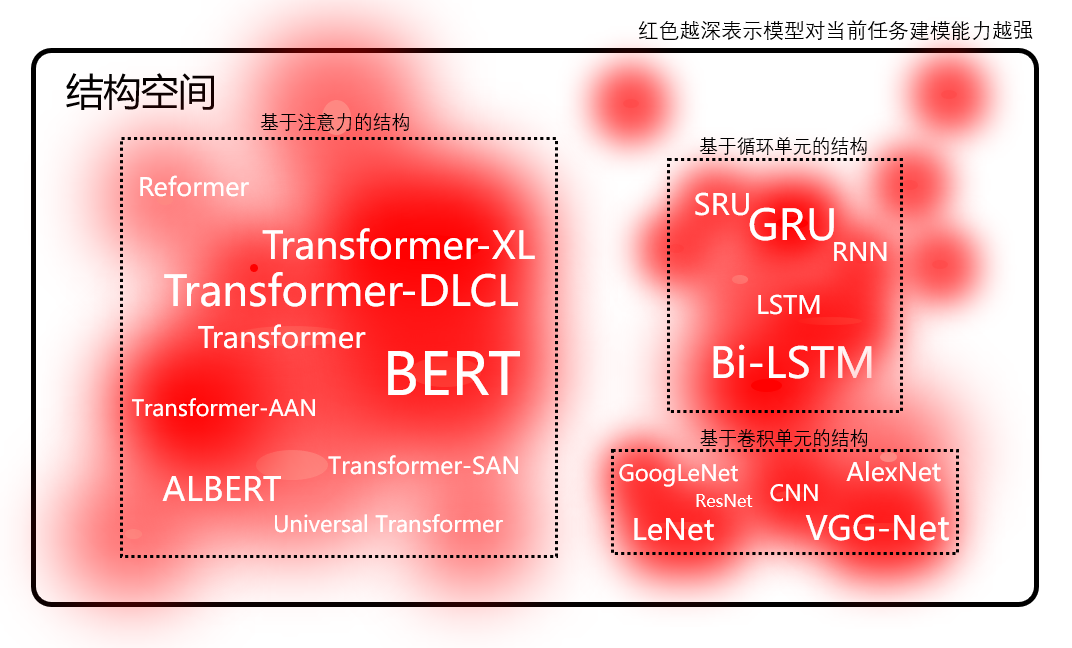
\includegraphics[scale=0.5]{./Chapter15/Figures/figure-relationship-between-structures-in-structural-space.jpg}
\caption{结构空间内结构之间的关系}
\label{fig:15-30}
\end{figure}
%-------------------------------------------

\parinterval 另一个很重要的问题是如何表示一个网络结构。在目前的结构搜索方法中,通常将模型结构分为整体框架和内部结构(元结构)两部分。整体框架将若干内部结构的输出按照特定的方式组织起来,最终得到模型输出。

\begin{itemize}
\vspace{0.5em}
\item {\small\bfnew{整体框架}}。如图\ref{fig:15-30}所示,整体框架一般基于经验进行设计。比如,对于包括机器翻译在内的自然语言处理任务而言,一般会更倾向于使用循环神经网络或Transformer模型的相关结构作为搜索空间\upcite{DBLP:conf/icml/SoLL19,DBLP:conf/iclr/ZophL17,DBLP:conf/iclr/LiuSY19}。
\vspace{0.5em}
\item 	{\small\bfnew{内部结构}}。对于内部结构的设计需要考虑到搜索过程中的最小搜索单元,以及搜索单元之间的连接方式。最小搜索单元指的是在结构搜索过程中可被选择的最小独立计算单元,在不同搜索空间的设计中,最小搜索单元的颗粒度各有不同,较小的搜索粒度主要包括如矩阵乘法、张量缩放等基本数学运算\upcite{DBLP:journals/corr/abs-2003-03384},更大粒度的搜索单元包括常见的激活函数以及一些局部结构,如ReLU、注意力机制等\upcite{DBLP:conf/acl/LiHZXJXZLL20,Chollet2017XceptionDL,DBLP:journals/taslp/FanTXQLL20}。不过,对于搜索颗粒度的问题,目前还缺乏有效的方法针对不同任务进行自动优化。
\vspace{0.5em}
\end{itemize}

%----------------------------------------------------------------------------------------
%    NEW SUBSUB-SECTION
%----------------------------------------------------------------------------------------

\subsubsection{2. 搜索策略}

\parinterval 在定义好搜索空间之后,如何进行网络结构的搜索也同样重要。该过程被称为搜索策略的设计,其主要目的是根据已找到的模型结构计算出下一个最有潜力的模型结构,为保证模型有效性,在一些方法中也会引入外部知识(如经验性的模型结构或张量运算规则)对搜索过程进行剪枝。目前常见的搜索策略一般包括基于进化算法的方法、基于强化学习的方法以及基于梯度的方法等等。

\begin{itemize}
\vspace{0.5em}
\item {\small\bfnew{进化算法}}。进化算法最初被用来对神经网络模型结构、以及其中的权重参数进行优化\upcite{DBLP:conf/icga/MillerTH89,DBLP:journals/tnn/AngelineSP94,stanley2002evolving}。随着最优化算法的发展,近年来,对于网络参数的学习开始更多地采用梯度下降的方式,但是进化算法依旧被用于对模型结构进行优化\upcite{DBLP:conf/icml/RealMSSSTLK17,DBLP:conf/iclr/ElskenMH19,DBLP:conf/iclr/LiuSVFK18}。从结构优化的角度来说,一般是将模型结构看做遗传算法中种群的个体,使用轮盘赌或锦标赛等抽取方式,对种群中的结构进行取样作为亲本,之后通过亲本模型的突变产生新的模型结构,最终对这些新的模型结构进行适应度评估。根据模型结构在校验集上的性能确定是否将其加入种群。
\vspace{0.5em}
\item 	{\small\bfnew{强化学习}}。强化学习方法在{\chapterthirteen}已经进行了介绍,这里可以将神经网络结构的设计看做是一种序列生成任务,使用字符序列对网络结构进行表述\upcite{DBLP:conf/iclr/ZophL17}。这种方法的执行过程如图\ref{fig:15-33}所示。其执行过程为由智能体对模型结构进行生成,之后将生成的结构应用于对应的任务(如机器翻译、语言建模等),根据模型在对应任务中的输出以及表现水平来进一步对智能体进行反馈,促使智能体生成更适用于当前任务的模型结构。

%----------------------------------------------
\begin{figure}[htp]
\centering

%%% outline
%-------------------------------------------------------------------------
\begin{tikzpicture}
\tikzstyle{node}=[minimum height=2.5em,minimum width=8em,draw,rounded corners=2pt,thick,drop shadow]

\node[node,fill=red!30] (n1) at (0,0){\small\bfnew{环境}};
\node[anchor=south,node,fill=blue!30] (n2) at ([yshift=5em]n1.north){\small\bfnew{智能体}};
\node[anchor=north,font=\footnotesize] at ([yshift=-0.2em]n1.south){(结构所应用于的任务)};
\node[anchor=south,font=\footnotesize] at ([yshift=0.2em]n2.north){(结构生成器)};

\draw[-latex,thick] ([yshift=.4em]n1.180) .. controls ([xshift=-3.4em,yshift=.4em]n1.180) and  ([xshift=-3.4em,yshift=-.4em]n2.180) .. node[right,font=\scriptsize,align=left]{\scriptsize\bfnew{奖励} \\ (对输出结果的评价)}([yshift=-.4em]n2.180);
\draw[-latex,thick] ([yshift=-.4em]n1.180) .. controls ([xshift=-4.4em,yshift=-.4em]n1.180) and  ([xshift=-4.4em,yshift=.4em]n2.180) .. node[left,font=\scriptsize,align=right]{\scriptsize\bfnew{状态} \\ (这个结构在任务中应 \\ 用后得到的输出结果)}([yshift=.4em]n2.180);
\draw[-latex,thick] (n2.0) .. controls ([xshift=4em]n2.0) and  ([xshift=4em]n1.0) .. node[right,font=\scriptsize,align=left]{\scriptsize\bfnew{动作} \\ (生成一个结构)}(n1.0);
\end{tikzpicture}





\caption{基于强化学习的结构搜索}
\label{fig:15-33}
\end{figure}
%-------------------------------------------

\vspace{0.5em}
\item 	{\small\bfnew{基于梯度的方法}}。这种方法的思想是在连续空间中对模型结构进行表示\upcite{DBLP:conf/iclr/LiuSY19},通常将模型结构建模为超网络中的结构参数,接下来使用基于梯度的方法对超网络中的参数进行优化,最终根据其中的结构参数离散出最终的模型结构,达到结构搜索的目的,整体过程如图\ref{fig:15-34}所示。基于梯度的方法十分高效,因此也受到了很多关注\upcite{DBLP:conf/cvpr/WuDZWSWTVJK19,DBLP:conf/iclr/XuX0CQ0X20,DBLP:conf/acl/LiHZXJXZLL20}。
\vspace{0.5em}

%----------------------------------------------
\begin{figure}[htp]
\centering

%%% outline
%-------------------------------------------------------------------------
\begin{tikzpicture}
\tikzstyle{node}=[minimum height=6em,inner sep=4pt,align=left,draw,font=\footnotesize,rounded corners=4pt,thick,drop shadow]

\node[node,fill=orange!30] (n1) at (0,0){\scriptsize\bfnew{超网络}: \\ [1ex] 模型结构参数 \\[0.4ex] 网络参数};
\node[anchor=west,node,fill=yellow!30] (n2) at ([xshift=4em]n1.east){\scriptsize\bfnew{优化后的超网络}: \\ [1ex]模型{\color{red}结构参数}(已优化) \\ [0.4ex]网络参数(已优化)};
\node[anchor=west,node,fill=red!30] (n3) at ([xshift=6em]n2.east){\scriptsize\bfnew{找到的模型结构}};

\draw[-latex,thick] (n1.0) -- node[above,align=center,font=\scriptsize]{优化后的\\超网络}(n2.180);
\draw[-latex,thick] (n2.0) -- node[above,align=center,font=\scriptsize]{根据结构参数\\离散化结构}(n3.180);
\draw[-latex,out=90,in=100,thick] ([xshift=-2em]n1.90) to node[above,font=\scriptsize]{参数优化}([xshift=2em]n1.90);
\end{tikzpicture}





\caption{基于梯度方法的结构搜索}
\label{fig:15-34}
\end{figure}
%-------------------------------------------

\end{itemize}

%----------------------------------------------------------------------------------------
%    NEW SUBSUB-SECTION
%----------------------------------------------------------------------------------------

\subsubsection{3. 性能评估}\label{subsubsec-15.4.2.3}

\parinterval 由于结构搜索过程中会产生大量的中间结构,因此需要快速评估这些结构的性能优劣,以保证在搜索中可以有效地挑选高质量的模型结构。对于该问题,可以从以下三个方面来考虑:

\begin{itemize}
\vspace{0.5em}
\item {\small\bfnew{数据以及超参数的调整}}。具体来说,可以用少量的数据训练模型,以便快速评估其性能\upcite{DBLP:conf/aistats/KleinFBHH17,DBLP:journals/corr/ChrabaszczLH17}。在超参数的调整方面,也可以通过减少模型训练轮数、减少模型的层数等方式来简化模型参数,达到加速训练、评估的目的\upcite{DBLP:conf/cvpr/ZophVSL18,Real2019AgingEF,DBLP:journals/corr/abs-1807-06906}。
\vspace{0.5em}
\item {\small\bfnew{现有参数的继承及复用}}。通过在现有的模型参数基础上,继续优化中间过程产生的模型结构,来加快待评价模型的收敛进程\upcite{DBLP:conf/icml/RealMSSSTLK17,DBLP:conf/iclr/ElskenMH19,DBLP:conf/aaai/CaiCZYW18}。这种方式无需从头训练搜索过程中产生的中间结构,通过“热启动”的方式对模型参数进行优化,能够大幅减少性能评估过程的时间消耗。
\vspace{0.5em}
\item {\small\bfnew{模型性能的预测}}。这种方式使用训练过程中的性能变化曲线来预估模型是否具有潜力,从而快速终止低性能模型的训练过程\upcite{DBLP:conf/ijcai/DomhanSH15,DBLP:conf/iclr/KleinFSH17,DBLP:conf/iclr/BakerGRN18}。
\vspace{0.5em}
\end{itemize}

%----------------------------------------------------------------------------------------
%    NEW SUB-SECTION
%----------------------------------------------------------------------------------------

\subsection{机器翻译任务下的结构搜索}

\parinterval 对于自然语言处理任务来说,网络结构搜索方法更多是在语言建模、命名实体识别等任务上进行尝试\upcite{DBLP:conf/acl/LiHZXJXZLL20,DBLP:conf/emnlp/JiangHXZZ19}。其中,大多数工作是在基于循环神经网络的模型结构上进行探索的,相较于目前在机器翻译领域中广泛使用的Transformer模型结构来说,这些搜索到的结构在性能上并没有体现出绝对的优势。此外,由于机器翻译任务的复杂性,针对基于Transformer的机器翻译模型的结构搜索方法会更少一些。不过仍有部分工作在机器翻译任务上取得了很好的表现。例如,在WMT19机器翻译比赛中,神经网络结构优化方法在多个任务上取得了很好的成绩\upcite{DBLP:conf/nips/LuoTQCL18,DBLP:conf/wmt/XiaTTGHCFGLLWWZ19}。对于结构搜索在机器翻译领域的应用,目前主要包括两个方面:分别是对模型性能的改进以及模型效率的优化。

%----------------------------------------------------------------------------------------
%    NEW SUBSUB-SECTION
%----------------------------------------------------------------------------------------

\subsubsection{1. 模型性能改进}

\parinterval 结构搜索任务中一个非常重要的目标是找到更加适用于当前任务的模型结构。目前来看,有两种思路:

\begin{itemize}
\vspace{0.5em}
\item {\small\bfnew{搜索模型中的局部结构}}。在机器翻译任务中,一种典型的局部模型结构搜索方法是面向激活函数的搜索\upcite{DBLP:conf/iclr/RamachandranZL18},该方法将激活函数看作是一元、二元函数的若干次复合。例如,Swish 激活函数就是一种被找到的新的激活函数,如下:
\begin{eqnarray}
f(x) &=& x \cdot \delta(\beta x) \\
\delta(z) &=& {(1 + \exp{(-z)})}^{-1}
\label{eq:15-60}
\end{eqnarray}

\noindent 相比于人工设计的激活函数ReLU而言,Swish函数在多个机器翻译任务取得了不错的效果。
\vspace{0.5em}
\item {\small\bfnew{搜索模型中局部结构的组合}}。在基于Transformer模型的网络结构搜索任务中,对于局部结构的组合方式的学习也受到了很多关注,其中包括基于进化算法的方法和基于梯度对现有Transformer模型结构的改良\upcite{DBLP:conf/icml/SoLL19,DBLP:journals/taslp/FanTXQLL20}。与前文所述的对局部结构的改良不同,此处更多地是对现有经验性的局部结构进行组合,找到最佳的整体结构。在模型结构的表示方法上,这些方法会根据先验知识为搜索单元设定一个部分框架,如每当信息传递过来之后先进行层标准化,之后再对候选位置上的操作使用对应的搜索策略进行搜索。另外这类方法也会在Transformer结构中引入多分支结构,一个搜索单元的输出可以被多个后续单元所使用,这种方式有效扩大了结构搜索过程中的搜索空间,能够在现有Transformer结构的基础上找到更优的模型结构。
\vspace{0.5em}
\end{itemize}

\parinterval 此外对模型结构中超参数的自动搜索同样能够有效提升模型的性能\upcite{DBLP:journals/corr/abs-2009-02070},这种方法在机器翻译中也有应用\upcite{Li2020NeuralMT}。

%----------------------------------------------------------------------------------------
%    NEW SUBSUB-SECTION
%----------------------------------------------------------------------------------------

\subsubsection{2. 模型效率优化}

\parinterval 网络结构搜索除了能够提高机器翻译模型性能之外,也能够优化模型的执行效率。从实用的角度出发,可以在进行结构搜索的同时考虑设备的计算能力,希望找到更适合运行设备的模型结构。同时,网络结构搜索也可以用来对大模型进行压缩,增加其在推断过程中的效率,这方面的工作不仅限于在机器翻译模型上,也有部分工作对基于注意力机制的预训练模型进行压缩。

\begin{itemize}
\vspace{0.5em}
\item {\small\bfnew{面向特定设备的模型结构优化}}。可以在结构优化的过程中将设备的算力作为一个约束\upcite{DBLP:conf/acl/WangWLCZGH20}。具体来说,可以将搜索空间中各种结构建模在同一个超网络中,通过权重共享的方式进行训练。使用设备算力约束子模型,并通过进化算法对子模型进行搜索,搜索到适用于目标设备的模型结构。该方法搜索到的模型能够在保证模型性能不变前提下获得较大的效率提升。
\vspace{0.5em}
\item {\small\bfnew{模型压缩}}。此外,在不考虑设备算力的情况下,也可以通过结构搜索方法对基于Transformer的预训练模型进行压缩。例如,将Transformer模型拆分为若干小组件,然后通过基于采样的结构搜索方法对压缩后的模型结构进行搜索,尝试找到最优且高效的推断模型\upcite{DBLP:journals/corr/abs-2008-06808}。类似的,也可以在基于BERT的预训练模型上通过结构搜索方法进行模型压缩,通过基于梯度的结构搜索方法,针对不同的下游任务将BERT模型压缩为小模型\upcite{DBLP:conf/ijcai/ChenLQWLDDHLZ20}。
\vspace{0.5em}
\end{itemize}

\parinterval 虽然由于算力等条件的限制,目前很多网络结构搜索方法并没有直接在机器翻译任务中进行实验,但是这些方法并没有被限制在特定任务上。例如,可微分结构搜索方法被成功地用于学习更好的循环单元结构,这类方法完全可以应用在机器翻译任务上。

\parinterval 此外,受到预训练模型的启发,网络结构预搜索可能是一个极具潜力的方向。例如,有研究人员在大规模语言模型上进行网络结构搜索\upcite{DBLP:conf/acl/LiHZXJXZLL20},然后将搜索到的模型结构应用于更多的自然语言处理任务中,这种方式有效提升了模型结构的可复用性。同时,相较于使用特定任务下受限的数据,从大规模单语数据中可以更充分地学习语言的规律,进而更好地指导模型结构的设计。此外,对于机器翻译任务而言,结构的预搜索同样是一个值得关注的研究方向。

%----------------------------------------------------------------------------------------
%    NEW SECTION
%----------------------------------------------------------------------------------------

\sectionnewpage
\section{小结及拓展阅读}

\parinterval 模型结构优化一直是机器翻译研究的重要方向。一方面,对于通用框架(如注意力机制)的结构改良可以服务于多种自然语言处理任务,另一方面,针对机器翻译中存在的问题设计相适应的模型结构也是极具价值的。本章节重点介绍了神经机器翻译中几种结构优化方法,内容涉及注意力机制的改进、深层神经网络的构建、句法结构的使用以及自动结构搜索等几个方面。此外,还有若干问题值得关注:

\begin{itemize}

\vspace{0.5em}
\item 多头注意力是近些年神经机器翻译中常用的结构。多头机制可以让模型从更多维度提取特征,也反应了一种多分支建模的思想。研究人员针对Transformer编码器的多头机制进行了分析,发现部分头在神经网络的学习过程中扮演了至关重要的角色,并且蕴含语言学解释\upcite{DBLP:journals/corr/abs-1905-09418}。 而另一部分头本身则不具备很好的解释,对模型的帮助也不大,因此可以被剪枝掉。而且也有研究人员发现,在Transformer模型中并不是头数越多模型的性能就越强。如果在训练过程中使用多头机制,并在推断过程中去除大部分头,可以在模型性能不变的前提下提高模型在CPU上的执行效率\upcite{Michel2019AreSH}。

\vspace{0.5em}
\item 此外,也可以利用正则化手段,在训练过程中增大不同头之间的差异\upcite{DBLP:conf/emnlp/LiTYLZ18}。或引入多尺度的思想,对输入的特征进行分级表示,并引入短语的信息\upcite{DBLP:conf/emnlp/HaoWSZT19}。还可以通过对注意力权重进行调整,来区分序列中的实词与虚词\upcite{DBLP:conf/emnlp/Lin0RLS18}。除了上述基于编码器端-解码器端的建模范式,还可以定义隐变量模型来捕获句子中潜在的语义信息\upcite{Su2018VariationalRN,DBLP:conf/acl/SetiawanSNP20},或直接对源语言和目标语言序列进行联合表示\upcite{Li2020NeuralMT}。

\vspace{0.5em}
\item 对Transformer等模型来说,处理超长序列是较为困难的。一种比较直接的解决办法是优化自注意力机制,降低模型计算复杂度。例如,采用了基于滑动窗口的局部注意力的Longformer模型\upcite{DBLP:journals/corr/abs-2004-05150}、基于随机特征的Performer\upcite{DBLP:journals/corr/abs-2006-04768}、使用低秩分解的Linformer\upcite{DBLP:journals/corr/abs-2009-14794}和应用星型拓扑排序的Star-Transformer\upcite{DBLP:conf/naacl/GuoQLSXZ19}。

\vspace{0.5em}
\end{itemize}
